% Options for packages loaded elsewhere
\PassOptionsToPackage{unicode}{hyperref}
\PassOptionsToPackage{hyphens}{url}
%
\documentclass[
]{book}
\usepackage{lmodern}
\usepackage{amssymb,amsmath}
\usepackage{ifxetex,ifluatex}
\ifnum 0\ifxetex 1\fi\ifluatex 1\fi=0 % if pdftex
  \usepackage[T1]{fontenc}
  \usepackage[utf8]{inputenc}
  \usepackage{textcomp} % provide euro and other symbols
\else % if luatex or xetex
  \usepackage{unicode-math}
  \defaultfontfeatures{Scale=MatchLowercase}
  \defaultfontfeatures[\rmfamily]{Ligatures=TeX,Scale=1}
\fi
% Use upquote if available, for straight quotes in verbatim environments
\IfFileExists{upquote.sty}{\usepackage{upquote}}{}
\IfFileExists{microtype.sty}{% use microtype if available
  \usepackage[]{microtype}
  \UseMicrotypeSet[protrusion]{basicmath} % disable protrusion for tt fonts
}{}
\makeatletter
\@ifundefined{KOMAClassName}{% if non-KOMA class
  \IfFileExists{parskip.sty}{%
    \usepackage{parskip}
  }{% else
    \setlength{\parindent}{0pt}
    \setlength{\parskip}{6pt plus 2pt minus 1pt}}
}{% if KOMA class
  \KOMAoptions{parskip=half}}
\makeatother
\usepackage{xcolor}
\IfFileExists{xurl.sty}{\usepackage{xurl}}{} % add URL line breaks if available
\IfFileExists{bookmark.sty}{\usepackage{bookmark}}{\usepackage{hyperref}}
\hypersetup{
  pdftitle={State-Space Models and Particle Filters},
  pdfauthor={Edoardo Marcelli; Roberto Colarieti; Alexei Verkhovtsev; Michele Bolla; Gabriele Romano; Benedetta Bruni},
  hidelinks,
  pdfcreator={LaTeX via pandoc}}
\urlstyle{same} % disable monospaced font for URLs
\usepackage{color}
\usepackage{fancyvrb}
\newcommand{\VerbBar}{|}
\newcommand{\VERB}{\Verb[commandchars=\\\{\}]}
\DefineVerbatimEnvironment{Highlighting}{Verbatim}{commandchars=\\\{\}}
% Add ',fontsize=\small' for more characters per line
\usepackage{framed}
\definecolor{shadecolor}{RGB}{248,248,248}
\newenvironment{Shaded}{\begin{snugshade}}{\end{snugshade}}
\newcommand{\AlertTok}[1]{\textcolor[rgb]{0.94,0.16,0.16}{#1}}
\newcommand{\AnnotationTok}[1]{\textcolor[rgb]{0.56,0.35,0.01}{\textbf{\textit{#1}}}}
\newcommand{\AttributeTok}[1]{\textcolor[rgb]{0.77,0.63,0.00}{#1}}
\newcommand{\BaseNTok}[1]{\textcolor[rgb]{0.00,0.00,0.81}{#1}}
\newcommand{\BuiltInTok}[1]{#1}
\newcommand{\CharTok}[1]{\textcolor[rgb]{0.31,0.60,0.02}{#1}}
\newcommand{\CommentTok}[1]{\textcolor[rgb]{0.56,0.35,0.01}{\textit{#1}}}
\newcommand{\CommentVarTok}[1]{\textcolor[rgb]{0.56,0.35,0.01}{\textbf{\textit{#1}}}}
\newcommand{\ConstantTok}[1]{\textcolor[rgb]{0.00,0.00,0.00}{#1}}
\newcommand{\ControlFlowTok}[1]{\textcolor[rgb]{0.13,0.29,0.53}{\textbf{#1}}}
\newcommand{\DataTypeTok}[1]{\textcolor[rgb]{0.13,0.29,0.53}{#1}}
\newcommand{\DecValTok}[1]{\textcolor[rgb]{0.00,0.00,0.81}{#1}}
\newcommand{\DocumentationTok}[1]{\textcolor[rgb]{0.56,0.35,0.01}{\textbf{\textit{#1}}}}
\newcommand{\ErrorTok}[1]{\textcolor[rgb]{0.64,0.00,0.00}{\textbf{#1}}}
\newcommand{\ExtensionTok}[1]{#1}
\newcommand{\FloatTok}[1]{\textcolor[rgb]{0.00,0.00,0.81}{#1}}
\newcommand{\FunctionTok}[1]{\textcolor[rgb]{0.00,0.00,0.00}{#1}}
\newcommand{\ImportTok}[1]{#1}
\newcommand{\InformationTok}[1]{\textcolor[rgb]{0.56,0.35,0.01}{\textbf{\textit{#1}}}}
\newcommand{\KeywordTok}[1]{\textcolor[rgb]{0.13,0.29,0.53}{\textbf{#1}}}
\newcommand{\NormalTok}[1]{#1}
\newcommand{\OperatorTok}[1]{\textcolor[rgb]{0.81,0.36,0.00}{\textbf{#1}}}
\newcommand{\OtherTok}[1]{\textcolor[rgb]{0.56,0.35,0.01}{#1}}
\newcommand{\PreprocessorTok}[1]{\textcolor[rgb]{0.56,0.35,0.01}{\textit{#1}}}
\newcommand{\RegionMarkerTok}[1]{#1}
\newcommand{\SpecialCharTok}[1]{\textcolor[rgb]{0.00,0.00,0.00}{#1}}
\newcommand{\SpecialStringTok}[1]{\textcolor[rgb]{0.31,0.60,0.02}{#1}}
\newcommand{\StringTok}[1]{\textcolor[rgb]{0.31,0.60,0.02}{#1}}
\newcommand{\VariableTok}[1]{\textcolor[rgb]{0.00,0.00,0.00}{#1}}
\newcommand{\VerbatimStringTok}[1]{\textcolor[rgb]{0.31,0.60,0.02}{#1}}
\newcommand{\WarningTok}[1]{\textcolor[rgb]{0.56,0.35,0.01}{\textbf{\textit{#1}}}}
\usepackage{graphicx,grffile}
\makeatletter
\def\maxwidth{\ifdim\Gin@nat@width>\linewidth\linewidth\else\Gin@nat@width\fi}
\def\maxheight{\ifdim\Gin@nat@height>\textheight\textheight\else\Gin@nat@height\fi}
\makeatother
% Scale images if necessary, so that they will not overflow the page
% margins by default, and it is still possible to overwrite the defaults
% using explicit options in \includegraphics[width, height, ...]{}
\setkeys{Gin}{width=\maxwidth,height=\maxheight,keepaspectratio}
% Set default figure placement to htbp
\makeatletter
\def\fps@figure{htbp}
\makeatother
\setlength{\emergencystretch}{3em} % prevent overfull lines
\providecommand{\tightlist}{%
  \setlength{\itemsep}{0pt}\setlength{\parskip}{0pt}}
\setcounter{secnumdepth}{5}
\def\code#1{\texttt{#1}}
\usepackage{babel}
\usepackage{amssymb}
\usepackage{amsfonts}
\usepackage{txfonts}
\usepackage{amsmath}
\usepackage{mathtools}
\usepackage[bindingoffset=1.5cm, left=3cm, right=3cm, top=3cm, bottom=3cm]{geometry}
\usepackage{graphicx}
\usepackage{MnSymbol} %allows to insert the QED at the end of the proofs
\usepackage{hyperref} %set the hyperlink to cite sections, equations...
\urlstyle{same}
\usepackage[toc,page]{appendix}
\usepackage{comment}
\usepackage{enumitem}
\usepackage{ntheorem}
\usepackage{lipsum}
\usepackage{xcolor}
\usepackage{mathtools}
\theoremstyle{break}
\newtheorem{thm}{Theorem}% theorem counter resets every \subsection
\renewcommand{\thethm}{\arabic{thm}}
\newtheorem{proposition}{Proposition}
\newtheorem{assumption}{Assumption}
\newtheorem{lemma}{Lemma}
\newtheorem{definition}{Definition}
\theoremstyle{nonumberplain}
\newtheorem{proof*}{Proof.}
\renewcommand{\P}{\mathbb{P}}
\newcommand\independent{\protect\mathpalette{\protect\independenT}{\perp}}
\def\independenT#1#2{\mathrel{\rlap{$#1#2$}\mkern2mu{#1#2}}}
\setcounter{MaxMatrixCols}{10}
\setlength{\oddsidemargin}{.0in}
\setlength{\textwidth}{6 in}
\setlength{\topmargin}{-.1in}
\setlength{\textheight}{8.1in}
\renewcommand{\baselinestretch}{1.5}
\newcommand{\E}{\mathbb E}
\newcommand{\Q}{\mathbb Q}
\newcommand{\M}{\mathbb M}
\newcommand{\R}{\mathbb R}
\newcommand{\B}{\mathcal B}
\newcommand{\X}{\mathcal X}
\newcommand{\Y}{\mathcal Y}
\newcommand{\Pd}{\mathbb P}
\newcommand{\N}{\mathcal N}
\newtheorem{algorithm}{Algorithm}[section]
\usepackage{float}
\floatplacement{figure}{}
\usepackage{float}
\usepackage{booktabs}
\usepackage{longtable}
\usepackage{array}
\usepackage{multirow}
\usepackage{wrapfig}
\usepackage{colortbl}
\usepackage{pdflscape}
\usepackage{tabu}
\usepackage{threeparttable}
\usepackage{threeparttablex}
\usepackage[normalem]{ulem}
\usepackage{makecell}
\usepackage{xcolor}

\title{\Huge State-Space Models and Particle Filters}
\author{Edoardo Marcelli \and Roberto Colarieti \and Alexei Verkhovtsev \and Michele Bolla \and Gabriele Romano \and Benedetta Bruni}
\date{10 Agosto, 2021}

\begin{document}
\frontmatter
\maketitle

\mainmatter
\tableofcontents

\chapter*{Introduction}

State-Space models represent an extremely interesting class of models
and they are used extensively, for instance, for inference and
forecasting in time-series and macroeconometric analysis. In fact, they
allow to model observational data as function of underlying states that
cannot be observed. For instance, in macroeconomic models GDP is usually
observed while the TFP sequence is the hidden state determining
output.\\
In this work we describe techniques, such as Kalman and Particle filter,
that allow to approximate probability distributions for the states from
the observed data. For example, from the sequence of observed GDP, it is
possible to ``filter'' the TFP factor.\\
Furthermore, it is possible to impose a Markov structure to State-Space
models, assuming that the states are Markov, i.e., the probability of
the current state depends on the entire sequence of past states only
through its first lag. The combination of State-Space and Markov
structures constitutes a powerful modeling assumption for inference and
forecasting. ~

Within the Monte Carlo (MC) methods, where inference is based on
repeated simulations that allow to approximate the target distributions
(needed to compute the estimator of interest), Particle Filter (PF)
Algorithms represent the most important class of procedures for
State-Space-Markov models. PF allows to sample states period-by-period,
updating sequentially the filtering distributions (i.e., the
distribution of current state conditional on all the sequence of
observations - up to the current period one -), incorporating the
information on the likelihood of the extracted states given the sequence
of observations, by means of re-weighting.\\
Moreover, the PF is a very general algorithm, since it can be applied to
non-linear models with non-Gaussian errors, while it does not allow for
a closed form solution. On the contrary, the Kalman Filter is a
filtering method that can be applied in the case of linear-Gaussian
State-Space-Markov models, and remains analytically tractable.~ In this
work we will describe both these algorithms, while our main focus
remains on Particle Filter. ~

In chapter \ref{MP_SSM_chapter} we define precisely Markov processes and
State-Space Models. In chapter \ref{KF_chapter} we describe the Kalman
Filter and in chapter \ref{PF_chapter} we analyze extensively the
Particle Filter. Finally, in chapter \ref{application_chapter}, we apply
these methods to stochastic volatility models.\\
Finally, we find it useful to integrate each section where an algorithm
is described and analyzed from a theoretical perspective with an
implementation subsection, using as an example a simple Random-Walk
State-Space model. In this way, the reader can visualize the codes and
the practical meaning of the Kalman and Particle Filter algorithms,
immediately after their theoretical description.

\chapter{Markov Processes and State-Space Models}\label{MP_SSM_chapter}

\section{Notation}

Let us fix the basic notation that will be employed henceforth. Upper
case letters, e.g.~\(X_t, Y_t,\) denote random variables, while lower
case letters denote the realizations. Finite sequences are made compact
using the semi-colon notation, e.g.~\(x_{0:t}=(x_0, x_1, \dots, x_t)\)
for some \(t \geq 0.\) The sets of outcomes are denoted by upper case
calligraphic letters, e.g.~\(\mathcal{X}, \mathcal{Y}.\) The
\(\sigma\)-algebra of a set \(\mathcal{X}\) reads
\(\mathcal{B}(\mathcal{X}).\) The pair
\((\mathcal{X}, \mathcal{B}(\mathcal{X}))\) is a measurable space. The
densities are represented with lower case cursive letters. For example,
the density of \(X_t\) in \(x_t\) is \(p_t^\theta(x_t),\) where
\(\theta\in\Theta\) is some (eventually known) vector, while the density
of \(X_t\) in \(x_t,\) given that \(X_{t-1}\) has previously taken value
\(x_{t-1},\) is \(p_t^\theta(x_t\mid x_{t-1}).\) Note that
\(p_t^\theta(x_t\mid x_{t-1})\) is a member of the parametric family
with parameters \((\theta, x_{t-1})\). The probability distribution of a
random variable \(X_t\) is represented by \(\mathbb{P}_t(dx_t),\) while
the probability distribution of a sequence \(X_{0:t}\) is represented by
\(\mathbb{P}_t(dx_{0:t}).\) The Dirac measure, i.e., the measure that
assigns probability \(1\) to the singleton \(\{x\},\) is denoted by
\(\delta_x(dy)\).The expectation operator is denoted by \(\mathbb{E},\)
where the section of \(\mathbb{E}\) at \(\mathbb{Q},\) i.e.,
\(\mathbb{E}_{\mathbb{Q}}\) denotes the operator computed with respect
to the probability distribution \(\mathbb{Q}.\) Let \(\varphi\) be a
function defined on the random variable \(X\propto\mathbb{Q}.\) Then, we
denote the expected value of \(\varphi(X)\) with \[
    \mathbb{E}_{\mathbb{Q}}[\varphi(X)]=
    \int_{\mathcal{X}}\varphi(x)\mathbb{Q}(dx).
\] Convergence in distribution is denoted with the symbol \(\implies.\)
So, \(X\implies\mathcal N(0,1)\) means that the random variable \(X\)
converges in distribution to a normal Gaussian.

\section{Markov Processes}

Let \((\mathcal{X}, \mathcal{B}(\mathcal{X}))\) and
\((\mathcal{Y}, \mathcal{B}(\mathcal{Y}))\) be two (eventually equal)
measurable spaces.\\

\begin{definition}
A function $P(x,dy): (\mathcal{X}, \mathcal{B}(\mathcal{X}))\rightarrow [0,1]$ such that 
\begin{itemize}
    \item for all $x\in\mathcal{X}, P(x,\cdot)$ is a probability measure on $(\mathcal{Y}, \mathcal{B}(\mathcal{Y})$, and 
    \item for all subsets $A\in\mathcal{B}(\mathcal{Y}),$ the map $x\mapsto P(x,A)$ is measurable in $\mathcal{B}(\mathcal{X})),$
\end{itemize}
is defined a probability kernel from $(\mathcal{X}, \mathcal{B}(\mathcal{X}))$ to $(\mathcal{Y}, \mathcal{B}(\mathcal{Y})).$
\end{definition}

Notice that for any random variables \(X_1\) and \(X_0=x_0,\) \[
    \mathbb{P}_1(dx_{0:1})=\mathbb{P}_0(dx_{0})P_1(x_0,dx_1),
\] where \(P_1(x_0,dx_1)\) is a probability kernel from
\((\mathcal{X}, \mathcal{B}(\mathcal{X}))\) to
\((\mathcal{X}, \mathcal{B}(\mathcal{X})).\) This remark, provides some
intuition about the link between probability kernels and conditional
probabilities. As a matter of fact, it is possible to show that for
given \(X_{0:1}\) with joint probability distribution
\(\mathbb{P}_1(dx_{0:1}),\)
\begin{equation}\label{prob_kern_condit_prob}
    \mathbb{P}_1(X_1\in dx_1\mid X_0=x_0)=P_1(x_0,dx_1).
\end{equation}

Probability kernels can be used to define Markov processes. Before
moving to the definition, we will introduce some important concepts.
Recall that given two measures \(\mathbb{M}\) and \(\mathbb{Q}\) defined
on a measurable space \((\mathcal{X}, \mathcal{B}(\mathcal{X})),\)
\(\mathbb{Q}\) is absolutely continuous with respect to \(\mathbb{M},\)
that is \(\mathbb{Q}\ll\mathbb{M},\) if for all sets
\(A\in\mathcal{B}(\mathcal{X})\) such that \(\mathbb{M}(A)=0,\) then it
must also hold that \(\mathbb{Q}(A)=0.\) If
\(\mathbb{Q}(A)/\mathbb{M}(A)\) is well-defined for all \(A,\) then the
Radon-Nikodym theorem guarantees that there exists a measurable function
\(w(x)\geq0\) such that \[
    w(x)=\frac{\mathbb{Q}(dx)}{\mathbb{M}(dx)}, 
\] meaning that, \[
    \mathbb{Q}(A)=\int_A w(x) \mathbb{M}(dx).
\]

Let \(P_1, P_2, \dots, P_T\) be a finite sequence of probability kernels
from \((\mathcal{X}, \mathcal{B}(\mathcal{X}))\) to
\((\mathcal{X}, \mathcal{B}(\mathcal{X})).\) Fix some
\(\mathbb{P}_0(dx)\) on \((\mathcal{X}, \mathcal{B}(\mathcal{X})).\)\\

\begin{definition}
A discrete-time Markov process is a sequence $X_{0:T}$ of random variables whose joint distribution can be written as
\begin{equation}
    \mathbb{P}_T(X_{0:T}\in dx_{0:T})=\mathbb{P}_0(dx_0)\prod\limits_{s=1}^T P_s(x_{s-1},dx_s).
\end{equation}
The set $\mathcal{X}$ is the state-space, $\mathbb{P}_0$ is the initial distribution and the probability kernel $P_t$ is the transition kernel.
\end{definition}

It is possible to show that for any \(t\in T,\) \[
\mathbb{P}_T(X_t\in dx_t\mid X_{0:t-1}\in dx_{0:t-1})=
\mathbb{P}_T(X_t\in dx_t\mid X_{t-1}=x_{t-1})=\mathbb{P}_t(x_{t-1},dx_t).
\] The first equality implies conditional independence. The second
equality implies that it is possible to identify conditional
distributions with transition kernels. Assume \(\mathbb{P}_t,\) with
\(t\leq T,\) is a sequence of probability measures. Then, the following
proposition holds.\\

\begin{proposition}
For all $t\leq T,$ 
$$
\mathbb{P}_T(dx_{0:t})=\mathbb{P}_0(dx_0)\prod\limits_{s=1}^t P_s(x_{s-1},dx_s)=\mathbb{P}_t(dx_{0:t}).
$$
\end{proposition}

This means that the marginal distribution of \(X_{0:t}\) with respect to
\(\mathbb{P}_T\) is \(\mathbb{P}_t.\)

\section{State-Space Models}\label{sec_state_space}

We now define \textit{State-Space models} as Markov processes that are
partially observed. Let \(X_t\in\mathcal X\) and \(Y_t\in\mathcal Y\)
and let \(\{(X_t,Y_t)\}\) be a stochastic process. To help intuition,
suppose that \(\{Y_t\}\) is observable, i.e., coincides with a sequence
of observations, while \(\{X_t\}\) is latent. Consider the initial
distribution \(\mathbb{P}_0(dx_0)\) and the probability kernels
\(P_t(x_{t-1},dx_t)\) and \(F_t(x_t,d_t)\), where \(t=1,2,\dots\).\\

\begin{definition}\label{state-space-def}
The process $\{(X_t,Y_t)\}$ is a State-Space model if the joint distribution of $(X_{0:T},Y_{0:T})$ is 
\begin{align*}
  \mathbb{P}_T(X_{0:T}\in dx_{0:T},Y_{0:T}\in dy_{0:T}) &= \mathbb{P}_0(dx_0)\prod\limits_{t=1}^T P_t(x_{t-1},dx_t)\prod\limits_{t=1}^T F_t(x_t,dy_t)\\
  &= [\mathbb{P}_0(dx_0)F_0(x_0,y_0)]\prod\limits_{t=1}^T[P_t(x_{t-1},dx_t)F_t(x_t,dy_t)] \\
  &= \mathbb{P}_T(dx_{0:T})\prod \limits_{t=1}^T F_t(x_t,dy_t).
\end{align*}
\end{definition}

From the second inequality, it is apparent that \(\{(X_t,Y_t)\}\) is a
Markov process with initial distribution
\([\mathbb{P}_0(dx_0)F_0(x_0,y_0)]\) and transition kernel
\(P_t(x_{t-1},dx_t)F_t(x_t,dy_t).\) The third equality, instead, shows
that, \(\{X_t\}\) has a marginal distribution
\[\mathbb{P}_T(dx_{0:T})=\mathbb{P}_0(dx_0)\prod_{t=1}^T P_t(x_{t-1},dx_t),\]
meaning that \(\{X_t\}\) is marginally distributed as a Markov process
with initial distribution \(\mathbb{P}_T(dx_{0:T})\) and transition
kernel \(P_t(x_{t-1},dx_t).\)

Assume now that there exists a dominating measures \(\nu(dy)\) such that
\(F_t(x_t,dy_t)=f_t(y_t\mid x_t)\nu(dy_t)\) for all \(t.\) Then by the
last equality of definition \ref{state-space-def}, the joint
distribution of \((X_{0:T},Y_{0:T})\) is
\begin{equation}\label{state-space-densities}
   \mathbb{P}_T(X_{0:T}\in dx_{0:T},Y_{0:T}\in dy_{0:T})=\mathbb{P}_T(dx_{0:T})\prod\limits_{t=0}^T f_t(y_t\mid x_t)\prod\limits_{t=0}^T\nu(dy_t).
\end{equation} Integrating away \(X_{0:T},\) one gets the marginal
density \begin{equation}\label{state-space-marginal-y}
  \mathbb{P}_T(dy_{0:T}) = \mathbb E_{\mathbb{P}_{t}}\big[\prod\limits_{s=0}^t f_s(y_s\mid X_s) \big] \prod\limits_{s=0}^t\nu(dy_s)
                = p_t(y_{0:t})\prod\limits_{s=0}^t\nu(dy_s),
\end{equation}\\
where \(p_t(y_{0:t})\) is the likelihood function. Dividing the
left-hand side of equation \ref{state-space-densities} by the left-hand
side of equation \ref{state-space-marginal-y} and the right-hand side of
equation \ref{state-space-densities} by the right-hand side of equation
\ref{state-space-marginal-y}, one obtains the distribution
\begin{equation}
\mathbb{P}_t(X_{0:t}\in dx_{0:t}\mid Y_{0:t}=y_{0:t})=\frac{1}{p_t(y_{0:t})}\big[\prod\limits_{s=0}^t f_s(y_s\mid X_s) \big]\mathbb{P}_t(dx_{0:t}).
\end{equation}

\chapter{Linear-Gaussian case}\label{KF_chapter}

\textit{Linear Gaussian models} are a class of popular state-space
models. A notable property of such models is that the filtering and
predictive distributions are analytically tractable, which makes such
models very convenient in applications.

Suppose that \(\mathcal X=\mathbb R^{d_x}\) and
\(\mathcal Y=\mathbb R^{d_y}.\) Let
\(U_t\thicksim\mathcal N(0,\Sigma_t)\) and
\(V_t\thicksim\mathcal N(0,\Lambda_t)\) be two independent white-noise
errors and assume the initial distribution
\(X_0\thicksim\mathcal N(0,\Sigma_0).\) We have a linear Gaussian model
if \begin{align}
X_t &= A_tX_{t-1}+U_t \\
Y_t &= B_tX_t + V_t.
\end{align} Note that \(X_t\mid X_{t-1}\) and \(Y_t\mid X_t\) are both
normally distributed.\\

\begin{lemma}\label{kalman-filter}
  Let $X\thicksim\mathcal N(m_0,C_0)$ and $Y\mid X\thicksim\mathcal N(BX,\Lambda)$, where $R$ and $Q_0$ are positive semi-definite matrices. 
  Then, it holds that
  \begin{align}
    X\mid Y=y&\thicksim\mathcal N(m_1,C_1),\\
    C_1&= C_0 (I_{d_x} - B'(B C_0 B'+ \Lambda)^{-1} B C_0) \\
    m_1&=[I_{d_x} - C_0 B'(B C_0 B'+ \Lambda)^{-1} B ]m_0 + C_0 B'(B C_0 B'+ \Lambda)^{-1}y.
  \end{align}
\end{lemma}
\begin{proof*}
   The lemma can be proved using Bayes' Theorem. Suppose $X\thicksim\mathcal N(m_0, C_0).$ It is easy to see that
\begin{equation} \label{normal-distrib-rewrite}
        p(x)\propto \text{exp}\Big(-\frac{1}{2}x'C_0^{-1}x + x'C_0^{-1}m_0\Big).
\end{equation}
Now, by Bayes' Theorem, 

    \begin{align*}
        p(x\mid Y=y)  &\propto p(x) p(y\mid x) \\
                    &\propto \text{exp}\Big(-\frac{1}{2}x' C_0^{-1}x + x' C_0^{-1}m_0-\frac{1}{2}(y-Bx)'\Lambda^{-1}(y-Bx)) \\
                    &\propto \text{exp}(-\frac{1}{2}x' C_0^{-1}x + x' C_0^{-1}m_0-\frac{1}{2}x' B' \Lambda^{-1}Bx+x' B' \Lambda^{-1}y)\\
                    &=\text{exp}(-\frac{1}{2}x'(C_0^{-1}+B' \Lambda^{-1}B)x+
                    x'(C_0^{-1}m_0+B' \Lambda^{-1}y)\Big).
    \end{align*}

Hence, it follows that 
\begin{equation*}
    C_1=Var(X\mid Y=y)= (C_0^{-1}+ B' \Lambda^{-1} B)^{-1}=C_0-C_0 B'(B C_0 B'+\Lambda)^{-1}B C_0
\end{equation*}
and 
\begin{equation*}
\begin{split}
        m_1 &=\mathbb E(X\mid Y=y) = C_1^{-1}(C_0^{-1}m_0+B' \Lambda^{-1}y)\\
            &= (C_0-C_0B'(B C_0B'+\Lambda)^{-1}B C_0)(C_0^{-1}m_0+B' \Lambda^{-1}y)\\
            &= m_0-C_0B'(B C_0B'+\Lambda)^{-1}B m_0 + C_0 B' \Lambda^{-1}y - C_0B'(B C_0B'+\Lambda)^{-1}B C_0 B' \Lambda^{-1}y \\
            &=[I_{d_x} - C_0 B'(B C_0 B'+ \Lambda)^{-1} B ]m_0 + C_0 B'(B C_0 B'+ \Lambda)^{-1}y.
\end{split}
\end{equation*}$\hfill\blacksquare$
\end{proof*}

Assume that
\(\mathbb{P}_{t-1}(dx_{t-1}\mid Y_{1:t-1}=y_{1:t-1})=\mathcal N(m_{t-1},C_{t-1}).\)
Then, using the transition equation of the latent variable, by the
linearity of the Gaussian distribution, we have that the predictive
distribution is \begin{equation}
\mathbb{P}_{t-1}(dx_{t}\mid Y_{1:t-1}=y_{1:t-1})=\mathcal N(A_tm_{t-1},A_tC_{t-1}A_t'+\Sigma_t).
\end{equation} Letting \(R_T=A_tC_{t-1}A_t'+\Sigma_t,\) and applying
lemma \ref{kalman-filter}, it follows that the filtering distribution is
\begin{align*}
  \mathbb{P}_{t}(X_t\in dx_{t}\mid Y_{1:t-1}&=y_{1:t-1})=\mathcal N(m_t,C_t), \text{ where} \\ C_t&=R_t[I_{d_x} - B_t'(B_tR_tB_t'+\Lambda_t)^{-1} B_tR_t] \\
  m_t &= [I_{d_x} - R_tB_t'(B_tR_tB_t'+\Lambda_t)^{-1} B_t]A_tm_{t-1}+R_tB_t'(B_tR_tB_t'+\Lambda_t)^{-1}y_t.
\end{align*}

In some situations, it is possible to linearize otherwise non-linear
models in order to employ this filtering method. There are, however,
cases where this is not possible or where the linearization is not
satisfactory. One such example is the stochastic volatility model. In
the following chapters, we will introduce powerful algorithms that can
be used in much more general settings.

\subsection{Implementation}\label{implementation}

The aim of this subsection is to provide a practical illustration of the
algorithms discussed in the main chapters. For the sake of simplicity we
use for implementations a random walk plus noise model, i.e.~the most
basic form of linear Gaussian state-space model.\\
\begin{align}
y_{t}|x_{t} & \sim N(x_{t},\sigma^{2}) \label{eq:1} \\
x_{t}|x_{t-1} & \sim N(x_{t-1},\tau^{2}) \label{eq:2} \\
x_{0} & \sim N(m_{0},C_{0})
\end{align} As already mentioned before, in this case the filtering
distribution can be computed in closed form solutions using the Kalman
filter. However, this toy example will be used also to illustrate more
involving filtering strategies described in this work. We believe indeed
that it represents a useful starting point to understand the logic of
the algorithms which may be eventually replicated when dealing with more
complex models.\\
The filtering strategy is applied to 50 simulated data. Figure
\ref{fig:myfig} shows the simulated true states sequence assuming as
data generating process the Equation \eqref{eq:2} with \(\tau^{2}=1\)
and simulated observed sequence process form Equation \eqref{eq:1} with
\(\sigma^{2}=1\).

\begin{figure}[H]

{\centering 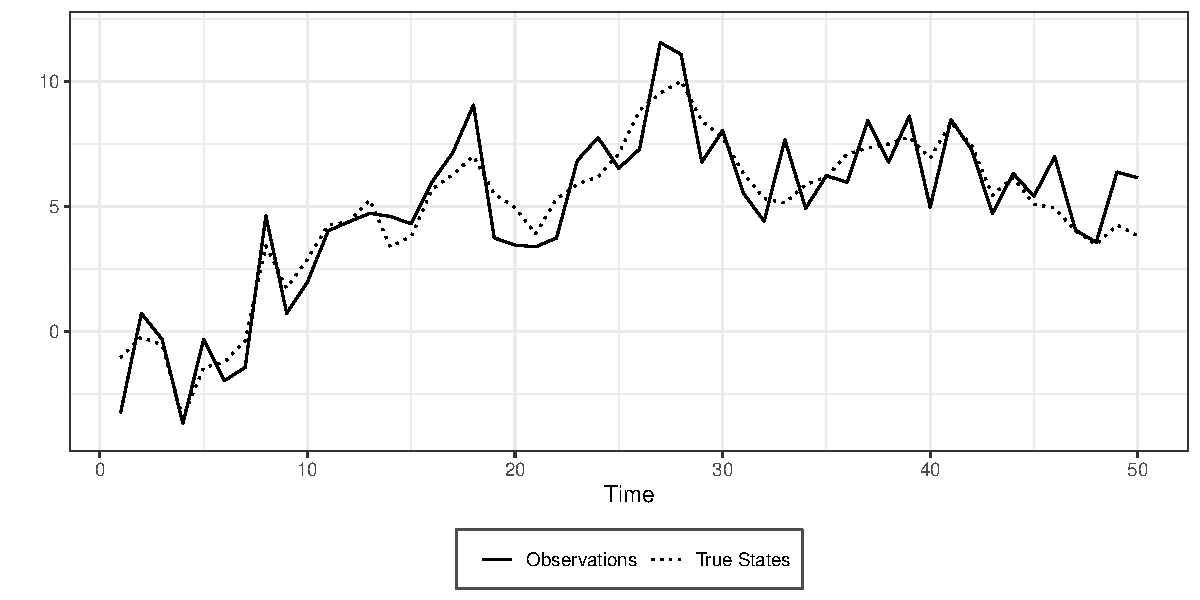
\includegraphics{prova_knit_finale_files/figure-latex/myfig-1} 

}

\caption{ Simulated random walk plus noise model}\label{fig:myfig}
\end{figure}

The Kalman Filter for this model is implemented as described below.

\begin{algorithm} Kalman Filter for Random Walk plus Noise Model
\begin{itemize}
\item Initialize $x_{0} \sim N(m_{0},C_{0})$
\item For $t=1,...,n$:
\begin{enumerate}
\item Compute the one-step-ahead state predictive distribution at time $t-1$, notice that if $t=1$ no data have been observed yet and therefore $x_{1}|x_{0}\sim N(a_{1},R_{1})$ otherwise
\begin{align*}
x_{t}|y_{1:t-1} & \sim N(a_{t},R_{t})\\
a_{t} & = m_{t-1}\\
R_{t} & = C_{t-1}+\tau^2
\end{align*}
\item Compute the filtering distribution at time $t$ as $p(x_{t}|y_{1:t}) \propto p(x_{t}|y_{1:t-1})p(y_{t}|x_{t})$, i.e. the product of the one-step-ahead state predictive distribution and the likelihood
\begin{align*}
x_{t}|y_{1:t} & \sim N(m_{t},C_{t}) \\
m_{t} & = \big(1-\frac{R_{t}}{R_{t}+\sigma^2}\big)a_{t}+\frac{R_{t}}{R_{t}+\sigma^2}y_{t} \\
C_{t} & = \frac{R_{t}}{R_{t}+\sigma^2}\sigma^2
\end{align*}
\end{enumerate}
\end{itemize}
\end{algorithm}

Our \texttt{DLM} function implement in R replicate this steps.\\

\hrule
\hrule

\texttt{DLM(data,sig2,tau2,m0,C0)}\\

\hrule

\textbf{Arguments}

\texttt{data} ~~the observed process. It has to be a vector or a
univariate time series.\\
\texttt{sig2} ~~the variance \(\sigma^{2}\) in observation equation\\
\texttt{tau2} ~~the variance \(\tau^{2}\) in state equation\\
\texttt{m0} ~~central value of the normal prior state distribution\\
\texttt{C0} ~~variance of the normal prior state distribution

\hrule
\hrule

\begin{Shaded}
\begin{Highlighting}[]
\NormalTok{DLM<-}\ControlFlowTok{function}\NormalTok{(data,sig2,tau2,m0,C0)\{}
\NormalTok{  n  =}\StringTok{ }\KeywordTok{length}\NormalTok{(data)}
\NormalTok{  m  =}\StringTok{ }\KeywordTok{rep}\NormalTok{(}\DecValTok{0}\NormalTok{,n)}
\NormalTok{  C  =}\StringTok{ }\KeywordTok{rep}\NormalTok{(}\DecValTok{0}\NormalTok{,n)}
  \ControlFlowTok{for}\NormalTok{ (t }\ControlFlowTok{in} \DecValTok{1}\OperatorTok{:}\NormalTok{n)\{}
    \ControlFlowTok{if}\NormalTok{ (t}\OperatorTok{==}\DecValTok{1}\NormalTok{)\{}
\NormalTok{      a =}\StringTok{ }\NormalTok{m0}
\NormalTok{      R =}\StringTok{ }\NormalTok{C0 }\OperatorTok{+}\StringTok{ }\NormalTok{tau2}
\NormalTok{    \}}\ControlFlowTok{else}\NormalTok{\{}
\NormalTok{      a =}\StringTok{ }\NormalTok{m[t}\DecValTok{-1}\NormalTok{]}
\NormalTok{      R =}\StringTok{ }\NormalTok{C[t}\DecValTok{-1}\NormalTok{] }\OperatorTok{+}\StringTok{ }\NormalTok{tau2}
\NormalTok{    \}}
\NormalTok{    A =}\StringTok{ }\NormalTok{R}\OperatorTok{/}\NormalTok{(R}\OperatorTok{+}\NormalTok{sig2)}
\NormalTok{    m[t] =}\StringTok{ }\NormalTok{(}\DecValTok{1}\OperatorTok{-}\NormalTok{A)}\OperatorTok{*}\NormalTok{a }\OperatorTok{+}\StringTok{ }\NormalTok{A}\OperatorTok{*}\NormalTok{y[t]}
\NormalTok{    C[t] =}\StringTok{ }\NormalTok{A}\OperatorTok{*}\NormalTok{sig2}
\NormalTok{  \}}
  \KeywordTok{return}\NormalTok{(}\KeywordTok{list}\NormalTok{(}\DataTypeTok{m=}\NormalTok{m,}\DataTypeTok{C=}\NormalTok{C))}
\NormalTok{\}}
\end{Highlighting}
\end{Shaded}

In Figure \ref{fig:myfig2} below filtered states estimated using Kalman
Filter with \(x_{0} \sim N(0,100)\) and \(\sigma^{2}=\tau^{2}=1\) are
compared to the true states values. Notice how closely the filtered
states follow the observations and the goodness of the approximation of
the true states. 95 percent credible intervals are computed as
\[[E(x_{t}|y_{1:t})-z_{1-\alpha/2}\sqrt{V(x_{t}|y_{1:t})},E(x_{t}|y_{1:t})+z_{1-\alpha/2}\sqrt{V(x_{t}|y_{1:t})}]\]

\begin{figure}[H]

{\centering 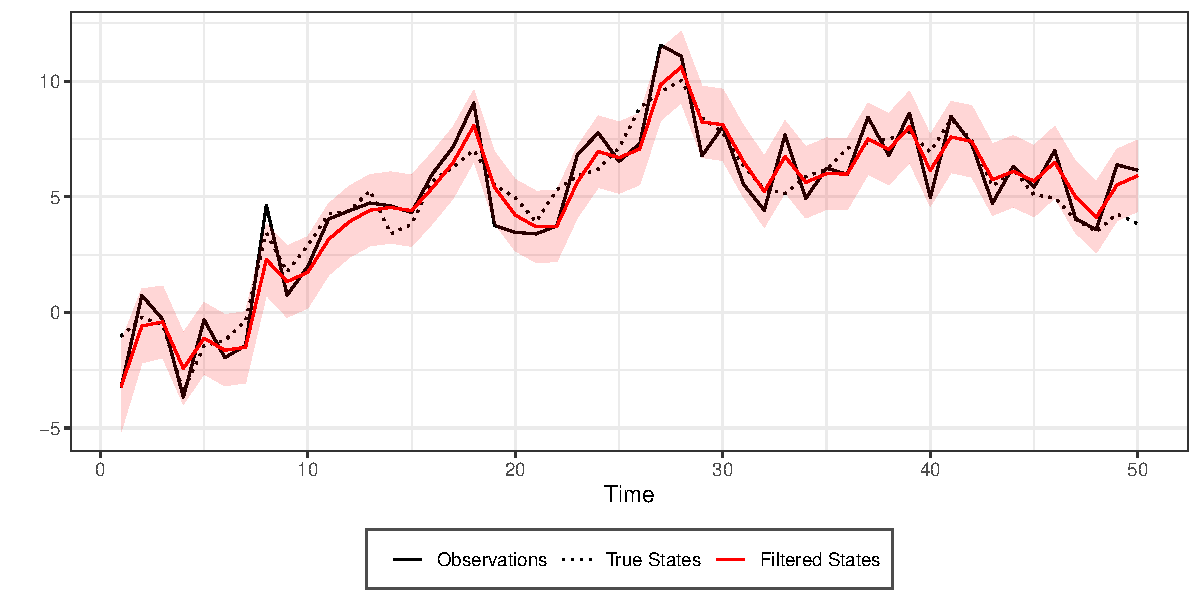
\includegraphics{prova_knit_finale_files/figure-latex/myfig2-1} 

}

\caption{Kalman Filtered States with credible interval (in red)}\label{fig:myfig2}
\end{figure}

The discussion of Kalman Filter will continue in the next sections where
we compare it to the Particle Filter.

\chapter{Particle Filter}\label{PF_chapter}

In the previous chapter we explained how the Kalman Filter is applied to
the case of a linear model with Gaussian errors to find closed-form
solution for the filtering and the predictive distributions.
Nonetheless, the majority of time-series models have a non-linear
structure and errors might follow non-Gaussian distributions.\\
In this chapter we describe \textit{particle filter} as an algorithm
that allows to update sequentially the filtering and the predictive
distributions in the non-linear and non-Gaussian case. Additionally, the
Kalman Filter can be seen as a special case of the more general particle
filter.\\
In section \ref{pf_intro} we introduce the fundamental notions of
\textit{importance sampling}, \textit{sequential importance sampling}
and \textit{resampling}. Then, in section \ref{pf_main} we describe
three particle filtering algorithms: the \textit{bootstrap}, the
\textit{guided} and the \textit{auxiliary particle filters}. Instead, in
section \ref{pf_liu_west} we describe the \textit{Liu and West filter},
when particle filtering is used to estimate model's parameters. Finally,
in section \ref{pf_converg} we establish some general convergence
results for Particle Filter - Monte Carlo estimators.

\section{Introductory notions: sampling and resampling}\label{pf_intro}

Let \(\varphi: \mathcal X\rightarrow \mathbb R\) be a measurable,
integrable and bounded real-valued function, where
\((\mathcal X,\mathcal B(\mathcal X),\mathbb Q)\) is a probability
space.\footnote{$\mathcal B(\mathcal X)$ is the Borel sigma-algebra of $\mathcal X$.}
Suppose that the probability measure \(\mathbb Q\) admits a density
\(q(x)\) with respect to some measure \(\nu(dx)\) and it is feasible to
sample from that density.\\
To estimate the expected value of \(\varphi\) with respect to the
density \(q\), the basic Monte Carlo (MC) method would require to sample
\(N\) times from the target density \(q\) and to compute the average of
the function \(\varphi\) values. \(\hat \varphi_{MC}\) is the standard
MC estimator: \begin{equation*}
   \hat \varphi_{MC}=\frac{1}{N} \sum_{n=1}^N\varphi (X^n)\approx \mathbb E_q(\varphi)~~~X^n\thicksim q(\cdot)
\end{equation*} However, in many circumstances either it is impossible
to sample from the target density or there exist another density - call
it \(m(\cdot)\) - different from \(q\) that produces ``more efficient''
estimates. In all the cases for which sampling takes place from a
distribution different from the ``correct'' (i.e., the true) one,
importance sampling and resampling methods can be applied (as augmented
versions of the standard MC algorithm).

\subsection{Importance sampling}

Let us consider two probability spaces:
\((\mathcal X,\mathcal B(\mathcal X),\mathbb Q)\) and
\((\mathcal X,\mathcal B(\mathcal X),\mathbb M)\) and let the measurable
function \(w:\mathcal X\rightarrow \mathbb R\) be proportional to the
Radom-Nikodym derivative between \(\mathbb Q\) and \(\mathbb M\), i.e.,
\(w(x)\propto\frac{\mathbb Q(dx)}{\mathbb M(dx)}\).\\
The following result represents the starting point for the idea of
importance sampling. \bigskip

\begin{lemma}\label{lemma_imp_sam_1}
For any measurable, integrable and bounded function $\varphi: \mathcal X\rightarrow \mathbb R$, the following holds:
\begin{equation}
    \mathbb E_\mathbb M(\varphi \cdot w)=\mathbb E_\mathbb Q(\varphi)\cdot \mathbb E_\mathbb M(w)
\end{equation}
\end{lemma}

\begin{proof*}
Note that $\mathbb Q(dx)=\frac{w(x)}{\mathbb E_\mathbb M(w)}\mathbb M(dx)$. Hence:
\begin{equation*}
    \mathbb E_\mathbb Q(\varphi)=\int_\mathcal X\varphi(x)\mathbb Q(dx)=\int_\mathcal X\varphi(x)\frac{w(x)}{\mathbb E_\mathbb M(w)}\mathbb M(dx)=\frac{\mathbb E_\mathbb M(\varphi \cdot w)}{\mathbb E_\mathbb M(w)}
\end{equation*}
$\hfill\blacksquare$
\end{proof*}

Lemma \ref{lemma_imp_sam_1} represents the key theoretical foundation of
\textbf{importance sampling} (IS), a numerical algorithm that allows to
sample from a \textit{proposal density} to estimate moments that are
computed with respect to the \textit{target density}, by means of
re-weighting the values of the target function \(\varphi\).\\
Adopting the previous notation, the target measure is \(\mathbb Q\),
while the proposal is \(\mathbb M\). IS requires to sample \(N\) values
from \(\mathbb M\), then to find the associated
\textit{normalized}\footnote{Weights are normalized when $\mathbb E_\mathbb M(W)=1$. In this case $W$ is the Radom-Nikodym derivative between $\mathbb Q$ and $\mathbb M$.}
weights \(W(X^n)\), finally to compute a weighted average of the values
taken by the function \(\varphi\). The IS is implemented according to
the following algorithm.

\begin{enumerate}
    \item Sample $N$ values from the proposal measure: $X^n\thicksim \mathbb M$ for $n=1,...,N$.
    \item Compute the associated normalized weights: $W(X^n)$ for $n=1,...,N$.
    \item Compute the estimator:
    \begin{equation*}
        \hat \varphi= \frac{1}{N} \sum_{n=1}^N\varphi (X^n)W(X^n).
    \end{equation*}
\end{enumerate}

Note that \(\hat \varphi\) is an unbiased estimator for the target of
inference \(\mathbb E_\mathbb Q(\varphi)\). In fact: \begin{equation*}
    \begin{split}
        \mathbb E_\mathbb M(\hat \varphi)=\frac{1}{N} \sum_{n=1}^N \mathbb E_\mathbb M(\varphi \cdot W)=\mathbb E_\mathbb M(\varphi \cdot W)=\mathbb E_\mathbb Q(\varphi)
    \end{split}
\end{equation*} where the last equality follows from lemma
\ref{lemma_imp_sam_1} and the fact that weights are normalized to 1.

\subsubsection{Auto-normalized IS}

Usually, the Radom-Nikodym derivative is known up to a normalizing
constant and the IS algorithm has to be described in more general terms.
In the previous section the \textit{normalized} weighting function
\(W(\cdot)\) was the Radom-Nikodym derivative of \(\mathbb Q\) with
respect to \(\mathbb M\). More generally, consider the function
\(w(x)\propto\frac{\mathbb Q(dx)}{\mathbb M(dx)}\), denoted as
\textit{importance function}, proportional to the derivative
\(W(\cdot)\).\\
In this case, weights have to be \textit{auto}-normalized to obtain the
IS - Monte Carlo estimator. The auto-normalized IS is implemented
according to the following procedure.

\begin{enumerate}
    \item Sample $N$ values from the proposal measure: $X^n\thicksim \mathbb M$ for $n=1,...,N$.
    \item Compute the associated \textit{un-normalized} weights: $w(X^n)$ for $n=1,...,N$.
    \item Normalize the weights, for $n=1,...,N$:
    \begin{equation*}
        W^n:=\frac{w(X^n)}{\sum_{m=1}^Nw(X^m)}.
    \end{equation*}
    \item Compute the estimator:
    \begin{equation*}
        \hat \varphi_{AN}=\sum_{n=1}^N\varphi (X^n)W^n.
    \end{equation*}
\end{enumerate}

While the auto-normalized estimator is biased (since \(W^n\) involves a
ratio of random variables), it is consistent (see \ref{pf_is_conv} for
details). ~\\
It is useful to interpret IS as an algorithm that allows to find an
approximation for the probability measure \(\mathbb Q\) as a weighted
average of Dirac measures for the sampled values (\(X^n\)):
\(\delta_{X^n}(dx)\) where the weights are the auto-normalized ones
(\(W^n\)). In particular: \begin{equation}
    \mathbb Q^N(dx):=\sum_{n=1}^NW^n\delta_{X^n}(dx), ~~~X^n\thicksim \mathbb M
\end{equation} Then, the auto-normalized IS estimator
\(\hat\varphi_{AN}\) is the expected value of the function \(\varphi\)
with respect to the approximating probability measure \(\mathbb Q^N\):
\begin{equation*}
    \begin{split}
        \mathbb E_{\mathbb Q^N}(\varphi)=&\int_\mathcal X\varphi(x)\mathbb Q^N(dx)=\int_\mathcal X\varphi(x)\sum_{n=1}^NW^n\delta_{X^n}(dx)=\\
       = &\sum_{n=1}^N\int_\mathcal X\varphi(x)W^n\delta_{X^n}(dx)=\sum_{n=1}^N\varphi (X^n)W^n=\hat \varphi_{AN}
    \end{split}
\end{equation*}

\subsubsection{Convergence of the IS estimator}\label{pf_is_conv}

We can show that the auto-normalized IS estimator is both consistent and
asymptotically normal.\\
Consider the auto-normalized IS estimator
\(\hat \varphi= \sum_{n=1}^N\varphi (X^n)W^n\). We can write:
\begin{equation*}
   \hat \varphi_{AN} - \mathbb E_{\mathbb Q}(\varphi)=\mathbb E_{\mathbb Q^N}(\varphi)-\mathbb E_{\mathbb Q}(\varphi)=\frac{N^{-1}\sum_{n=1}^Nw(X^n)[\varphi(X^n)-\mathbb E_{\mathbb Q}(\varphi)]}{N^{-1}\sum_{n=1}^Nw(X^n)}
\end{equation*} Let
\(\bar \varphi(X):=\varphi(X)-\mathbb E_{\mathbb Q}(\varphi)\). Applying
the CLT to the numerator, assuming that
\(\mathbb E_{\mathbb M}(w^2\bar\varphi^2)<+\infty\), we get:
\begin{equation}
    \sqrt{N}\Bigg\{\frac{1}{N}\sum_{n=1}^Nw(X^n)\bar \varphi (X^n)\Bigg\}\implies \mathcal N\big(0,\mathbb E_{\mathbb M}(w^2\bar\varphi^2)\big)\label{is_conv_clt}
\end{equation} where \(\implies\) denotes convergence in distribution.
Instead, for the denominator the strong LLN implies that:
\begin{equation}
    \frac{1}{N}\sum_{n=1}^Nw(X^n)\xrightarrow{\text{a.s.}} \mathbb E_{\mathbb M}(w) \label{is_conv_lln}
\end{equation} Applying Slutsky's theorem, together with
\eqref{is_conv_clt} and \eqref{is_conv_lln}, we obtain: \begin{equation}
   \sqrt{N}\big[  \hat \varphi_{AN} - \mathbb E_{\mathbb Q}(\varphi)\big] \implies \mathcal N\Bigg(0,\frac{\mathbb E_{\mathbb M}(w^2\bar\varphi^2)}{[\mathbb E_{\mathbb M}(w)]^2}\Bigg)
\end{equation} Therefore, the IS (auto-normalized) estimator for
\(\varphi\) is asymptotically normal. Consistency can be proved in an
analogous way, applying the strong LLN and lemma \ref{lemma_imp_sam_1}:
\begin{equation}
    \frac{1}{N}\sum_{n=1}^Nw(X^n) \varphi (X^n)\xrightarrow{\text{a.s.}}  \mathbb E_\mathbb M(\varphi \cdot w)=\mathbb E_\mathbb Q(\varphi)\cdot \mathbb E_\mathbb M(w)
\end{equation} Together with \eqref{is_conv_lln}, we get strong
convergence of the estimator (that implies consistency).
\begin{equation}
   \hat \varphi_{AN}=\sum_{n=1}^NW^n \varphi (X^n)\xrightarrow{\text{a.s.}}  \mathbb E_\mathbb Q(\varphi)
\end{equation}

\subsubsection{Effective Sample Size}

A common measure of efficiency for IS is the
\textit{effective sample size} (ESS), defined as: \begin{equation*}
    ESS(W^{1:N}):=\frac{1}{\sum_{n=1}^N(W^n)^2}=\frac{[\sum_{n=1}^N w(X^n)]^2}{\sum_{n=1}^N(w(X^n))^2}
\end{equation*} Observe that the \(ESS\) lies in the interval \([1,N]\).
For instance, if \(W^n=1/N\), as in the case of the standard MC method,
\(ESS=N\).\\
It is possible to relate the \(ESS\) to the variance of the importance
function. In fact: \begin{equation*}
    \frac{N}{ESS}=1+\frac{N^{-1}\sum_{n=1}^N(w(X^n))^2-\big[N^{-1}\sum_{n=1}^N w(X^n)\big]^2}{\big[N^{-1}\sum_{n=1}^N w(X^n)\big]^2}
\end{equation*} The second term in the numerator of the previous formula
is the square of the coefficient of variation (i.e., the ratio between
the variance and the squared mean) of the un-normalized weights. It is
clear that a lower \(ESS\) is associated with a higher variance for the
weights.

\subsection{Sequential Importance Sampling}\label{seq_impt_sampling}

When dealing with state-space models, the importance sampling algorithm
has to be applied dynamically and the importance weights are updated
period-by-period. To illustrate the relevance of the
\textit{sequential importance sampling} (SIS) algorithm, we consider a
two-period stochastic process.~\\
Let us consider the approximation of the measure \(\mathbb Q_0\)
obtained at time 0 through IS from the measure \(\mathbb M_0\):
\begin{equation*}
    \mathbb Q_0^N(dx_0)=\sum_{n=1}^NW_0^n\delta_{X_0^n}(dx_0),~~\text{with } X_0^n\thicksim \mathbb M_0,~~\text{and }  W_0^n:=\frac{w_0(X_0^n)}{\sum_{m=1}^Nw_0(X_0^m)}.
\end{equation*} Moreover, let \(M_1(x_0,dx_1)\) be the transition
kernel. We want to update, sequentially, the approximating measure
\(\mathbb Q_0\) to obtain an approximation of the measure:
\begin{equation*}
    \mathbb Q_{1}(dx_{0:1})=\mathbb Q_0(dx_0)M_1(x_0,dx_1)
\end{equation*} SIS works according to the following algorithm.

\begin{enumerate}
    \item Sample $N$ values for $X_0$ from the proposal measure $\mathbb M_0$: $X_0^n\thicksim \mathbb M_0$ for $n=1,...,N$.
    \item Sample $N$ values for $X_1$ from the transition kernel $M_1$: $X_1^n\thicksim M_1(X_0^n,dx_1)$ for $n=1,...,N$.
    \item Compute the auto-normalized weights. In this case, they are computed taking into account only time 0 sampled observations since $X_1^n$ is sampled from the correct distribution: $W_1^n=W_0^n$.
\end{enumerate}

Therefore, the particle approximation of \(\mathbb Q_{1}(dx_{0:1})\) is:
\begin{equation*}
      \mathbb Q_{1}^N(dx_{0:1})=\sum_{n=1}^NW_0^n\delta_{X_0^n}(dx_0)M_1(X_0^n,dx_1)
\end{equation*}

\subsection{Sequential Importance Resampling}

A second approach can be used when sampling has to be done sequentially:
\textit{sequential importance resampling} (SIR). Differently from SIS,
an intermediate resampling stage takes place, in which time 0 values are
sampled with replacement according to a given resampling strategy
(usually, sampling indexes from a multinomial distribution with
probabilities equal to the weights computed through IS at time 0).\\
While in the SIS all the particles (i.e., the sampled values)
``survive'', with the ``risk'' that particles associated with small
weights are carried-over (in the sense that sampling in period 1 occurs
from the kernel \(M_1(X_0^n,dx_1)\)), the same does not occur in SIR. In
this second algorithm, particles with larger weights are more likely to
be resampled and be used to ``generate" the particles in the next
period.\\
We describe the SIR more formally, focusing on the previous two-period
case.

\begin{enumerate}
    \item Sample $N$ values $X_0$ from the proposal measure $\mathbb M_0$: $X_0^n\thicksim \mathbb M_0$ for $n=1,...,N$.
    \item Compute the weights $W_0^n$ for $n=1,...,N$.
    \item Sample $N$ indexes $(A_1^1,...A_1^N)$ from a multinomial distribution such that for all $j=1,...N$, $Pr(\{A_1^j=n\})=W_0^n$, for all $n=1,...N$.
    \item Build a new time 0 sample, using the values for $X_0$ associated to the previously extracted indexes $(A_1^n)_{n}$: $(X_0^{A_1^1},...,X_0^{A_1^N})$.
    \item Sample $N$ values for $X_1$ from the transition kernel $M_1$: $X_1^n\thicksim M_1(X_0^{A_1^n},dx_1)$ for $n=1,...,N$.
\end{enumerate}

Steps 3-4 constitute the actual resampling ones. At this point, let us
define the new two-period sequence
\(\tilde X_{0:1}^n:=(X_0^{A_1^n},X_1^n)\). Then, the particle
approximation for the joint distribution of \((X_0,X_1)\) becomes:
\begin{equation*}
     \mathbb Q_{1}^N(dx_{0:1})=\frac{1}{N}\sum_{n=1}^N\delta_{\tilde X_{0:1}^n}(dx_{0:1})
\end{equation*} Note that, after resampling occurred, each particle
\(\tilde X_{0:1}^n:=(X_0^{A_1^n},X_1^n)\) has the same probability
weight.\\
To understand the logic of the previous statement, let us assume that
both \(\mathbb Q_0\) and \(\mathbb M_0\) admit densities \(q_0\),
\(m_0\) with respect to the same dominating measure \(\nu(dx_0)\) and
that the transition kernel \(M_1\) also admits the density \(m_1\).
Consider the sequential updating for the weights: \begin{equation}
    W^n_1=\frac{\mathbb Q_1(dx_{0:1})}{\mathbb M_1(dx_{0:1})}\propto \frac{q_0(x_0^{A_1^n})}{Pr(A_1^n)\cdot m_0(x_0^{A_1^n})}\cdot \frac{m_1(x_1^n|x_0^{A_1^n})}{m_1(x_1^n|x_0^{A_1^n})}
=\underbrace{\frac{q_0(x_0^{A_1^n})}{ m_0(x_0^{A_1^n})}}_{W_0^n}\cdot \underbrace{\frac{1}{Pr(A_1^n)}}_{1/W_0^n}=1\label{sis_update}
\end{equation} where \(\mathbb M_1\) denotes the probability measure for
the extraction of the particle \(\tilde x_{0:1}^n\) according to SIR.
\(\mathbb M_1\) (second equality sign in the previous formula) can be
rewritten as the product between the kernel for \(x_1^n\) given
\(x_0^{A_1^n}\) and the probability of \(x_0^{A_1^n}\) itself. This last
probability can also be rewritten as the product between the proposal
density \(m_0\) from which \(X_0\) is extracted and the probability that
it is sampled again when resampling occurs.

\subsection{SIS vs SIR}

The choice between the two sequential sampling strategies (SIS and SIR)
has significant implications in terms of computational cost and variance
of the importance weights. In fact, it is clear that SIR is more costly
computationally since it requires an intermediate resampling step.
Nonetheless, SIS suffers from the problem knonw as
\textit{curse of dimensionality}, i.e., the fact that the \(ESS\)
collapses over time as the variance of the weights diverges.\\
Consider an extension of SIS to a \(T\)-period model and let us assume
that the target and the proposal kernels admit densities, respectively,
\(q_t\) and \(m_t\) with respect to the same dominating measures (this
implies that the joint
distributions\footnote{Let us denote the joint distributions with $q_t$ and $m_t$ too, with some abuse of notation.}
admit a density too). Then, weights, for every \(t=1,...,T\), are
updated according to: \begin{equation}
    w_t^n\propto \frac{q_t(x_{0:t}^n)}{m_t(x_{0:t}^n)}\propto \underbrace{\frac{q_{t-1}( x_{0:t-1}^n)}{m_{t-1}(x_{0:t-1}^n)}}_{\propto w_{t-1}^n}\cdot \frac{q_t( x_t|x_{t-1}^n)}{m_t(x_t|x_{t-1}^n)}\propto 
    w_{t-1}^n\cdot\frac{q_t( x_t|x_{t-1}^n)}{m_t(x_t|x_{t-1}^n)}\label{sis_update}
\end{equation} Intuitively, equation \eqref{sis_update} suggests that
over time new variance is added from the incremental weights (i.e., the
updating factor \(q_t( x_t|x_{t-1}^n)/m_t( x_t|x_{t-1}^n)\)) determining
the curse of dimensionality issue. Instead, when resampling takes place,
since the past weights \(w_{t-1}\) are reset to be equal across them all
the variance of \(w_t\) inherited from the past is shut-down and the
only source of variability at each stage comes from the incremental
weights.

\section{Particle Filter}\label{pf_main}

Let us consider the standard state-space model introduced previously
(see \ref{sec_state_space}). \textit{Particle filter} (PF) is a
numerical algorithm that is used to obtain approximations for the
filtering - \(\mathbb P_t (dx_t|y_{1:t})\) - and the prediction -
\(\mathbb P_t (dx_t|y_{1:t-1})\) - distributions for inference in
state-space models.~\\
In a state-space model sampling sequentially from the transition kernels
for the states is not enough to obtain good approximations since the
observation sample (\(y_{1:T}\)) contains information about the
underlying states through the likelihood function \(f_t(y_t|x_t)\).
Observations constitute signals for the model's states.\\
Therefore, the conditional distribution of the states, given the
observed data - \(\mathbb P_t(dx_{1:t}|y_{1:t})\) - changes over time as
new data points become available. The PF algorithm allows to incorporate
sequentially the new data to obtain new approximations for this
distribution (and for the filtering and prediction ones).\\
In general, at each step of the algorithm, states are sampled
sequentially from the proposal measure, call it \(\mathbb M_t\), and
importance auto-normalized weights are computed as the Radom-Nikodym
derivative of the target \(\mathbb P_t\) with respect to the proposal
\(\mathbb M_t\). Moreover, the Markov properties of the sequence of the
states allows to update sequentially the importance weights.~\\
We will analyse three different types of particle filtering procedures:
\textit{bootstrap}, \textit{guided} and
\textit{auxiliary particle filters}, that differ between them with
respect to their scope and efficiency.

\subsection{Degeneracy of the SIS in Particle Filter}

Usually, PF requires a resampling step at each stage of the algorithm.
Recall that, in general, resampling determines a trade-off between the
increase in the variance at the resampling stage and a decrease in the
variance when future states are sampled from the transition kernel.\\
``Dead'' particles (i.e., those with small weights) are likely to be
removed when resampling takes place and past weights get ``reset"
(usually, they are set to be equal to \(1/N\)). Otherwise, the
\textit{curse of dimensionality} problem will emerge and the variance of
the weights will diverge over time as new updates occur
period-by-period. Next, we show an example of a PF where SIS is used:
note that the \(ESS\) drops dramatically after few periods, meaning that
the variance of the importance weights diverges. This motivates the use
of a SIR structure for the PF algorithm.~\\
Lastly, it is now common practice to use a mixed approach with respect
to resampling (recall that resampling has an additional computational
cost). Generally, resampling is done \textit{adaptively}, when some
condition is met. A standard criterion that is used (and that we adopt
in our implementations of the PF) is to resample when the \(ESS\) drops
below some threshold \(ESS_{min}\in [1,N]\): \begin{equation}
    ESS(W_{t-1}^{1:N})<ESS_{min}
\end{equation}

\subsection{Implementation}

Consider again the random walk plus noise model of section
\ref{implementation}, the challenge here is to estimate the filtered
states using a Sequential Importance Sampling algorithm. The main idea
of the SIS applied to this univariate linear gaussian model is described
in the following algorithm. We indicate with \(n\) the sample size of
time observations and with \(N\) the generated sample size for each step
of the Sequenial Monte Carlo.

\begin{algorithm} SIS filter for Random Walk plus Noise Model
\begin{itemize}
\item Let $\{(x_{0},w_{0})^{(i)}\}_{i=1}^{N}$ summarize $p(x_{0}|y_{0})$ such that, for example, $E(g(x_{0})|y_{0}) \approx \sum_{i=1}^{N}w_{0}^{(i)}g(x_{0}^{(i)})$. In particular, initialize $(x_{0}^{(1)},...,x_{0}^{(N)})$ form $N(m_{0},C_{0})$ and set $w_{0}^{(i)}=N^{-1} \ \forall \ i=1,...,N$.
\item For $t=1,...,n$:
\begin{enumerate}
\item Draw $x_{t}^{(i)} \sim N(x_{t-1}^{(i)},\tau^2) \ \ i=1,...,N$ such that $\{(x_{t},w_{t-1})^{(i)}\}_{i=1}^{N}$ summarizes $p(x_{t}|y_{t-1})$
\item Set $w_{t}^{(i)} = w_{t-1}^{(i)}f_{N}(y_{t};x_{t}^{(i)},\sigma^2) \ \ i=1,...,N$ such that $\{(x_{t},w_{t})^{(i)}\}_{i=1}^{N}$ summarizes $p(x_{t}|y_{t})$
\item Set $p(x_{t}|y_{t})=\sum_{i=1}^{N}w_{t}^{(i)}\delta_{x_{t}^{(i)}}$
\end{enumerate}
\end{itemize}
\end{algorithm}

Our \texttt{SISfun} function implemented in R replicate this steps.\\

\hrule
\hrule

\texttt{SISfun(data,N,m0,C0,tau,sigma)}\\

\hrule

\textbf{Arguments}

\texttt{data} ~~the observed process. It has to be a vector or a
univariate time series.\\
\texttt{N} ~~number of particles generated at each step\\
\texttt{m0} ~~central value of the normal prior state distribution\\
\texttt{C0} ~~variance of the normal prior state distribution\\
\texttt{tau} ~~the standard deviation \(\tau\) in state equation\\
\texttt{sigma} ~~the standard deviation \(\sigma\) in observation
equation

\hrule
\hrule

\begin{Shaded}
\begin{Highlighting}[]
\NormalTok{SISfun<-}\ControlFlowTok{function}\NormalTok{(data,N,m0,C0,tau,sigma)\{}
\NormalTok{  xs<-}\OtherTok{NULL}
\NormalTok{  ws<-}\OtherTok{NULL}
\NormalTok{  ess<-}\OtherTok{NULL}
\NormalTok{  x  =}\StringTok{ }\KeywordTok{rnorm}\NormalTok{(N,m0,}\KeywordTok{sqrt}\NormalTok{(C0))}
\NormalTok{  w  =}\StringTok{ }\KeywordTok{rep}\NormalTok{(}\DecValTok{1}\OperatorTok{/}\NormalTok{N,N)}
  \ControlFlowTok{for}\NormalTok{(t }\ControlFlowTok{in} \DecValTok{1}\OperatorTok{:}\KeywordTok{length}\NormalTok{(data))\{}
\NormalTok{    x    =}\StringTok{ }\KeywordTok{rnorm}\NormalTok{(N,x,tau)                   }
\NormalTok{    w    =}\StringTok{ }\NormalTok{w}\OperatorTok{*}\KeywordTok{dnorm}\NormalTok{(data[t],x,sigma)         }
\NormalTok{    xs =}\StringTok{ }\KeywordTok{rbind}\NormalTok{(xs,x)}
\NormalTok{    ws =}\StringTok{ }\KeywordTok{rbind}\NormalTok{(ws,w)}
    
\NormalTok{    wnorm=}\StringTok{ }\NormalTok{w}\OperatorTok{/}\KeywordTok{sum}\NormalTok{(w)                         }
\NormalTok{    ESS  =}\StringTok{ }\DecValTok{1}\OperatorTok{/}\KeywordTok{sum}\NormalTok{(wnorm}\OperatorTok{^}\DecValTok{2}\NormalTok{)                   }
    
\NormalTok{    ess =}\KeywordTok{rbind}\NormalTok{(ess,ESS)}
\NormalTok{  \}}
  
  \KeywordTok{return}\NormalTok{(}\KeywordTok{list}\NormalTok{(}\DataTypeTok{xs=}\NormalTok{xs,}\DataTypeTok{ws=}\NormalTok{ws,}\DataTypeTok{ess=}\NormalTok{ess))}
\NormalTok{\}}
\end{Highlighting}
\end{Shaded}

We have already discussed the reasons why the SIS algorithm does not
provide a good strategy in the filtering problem. We provide a graphical
intuition of what happens when we use such filtering strategy on a
simulated dataset. We decide to set \(N=1000\), \(m_{0}=0\),
\(C_{0}=100\) and \(\tau=\sigma=1\). The following two plots show a
clear degeneration of the effective sample size and bad fit of filtered
states with respect to the true values.

\begin{figure}[H]

{\centering 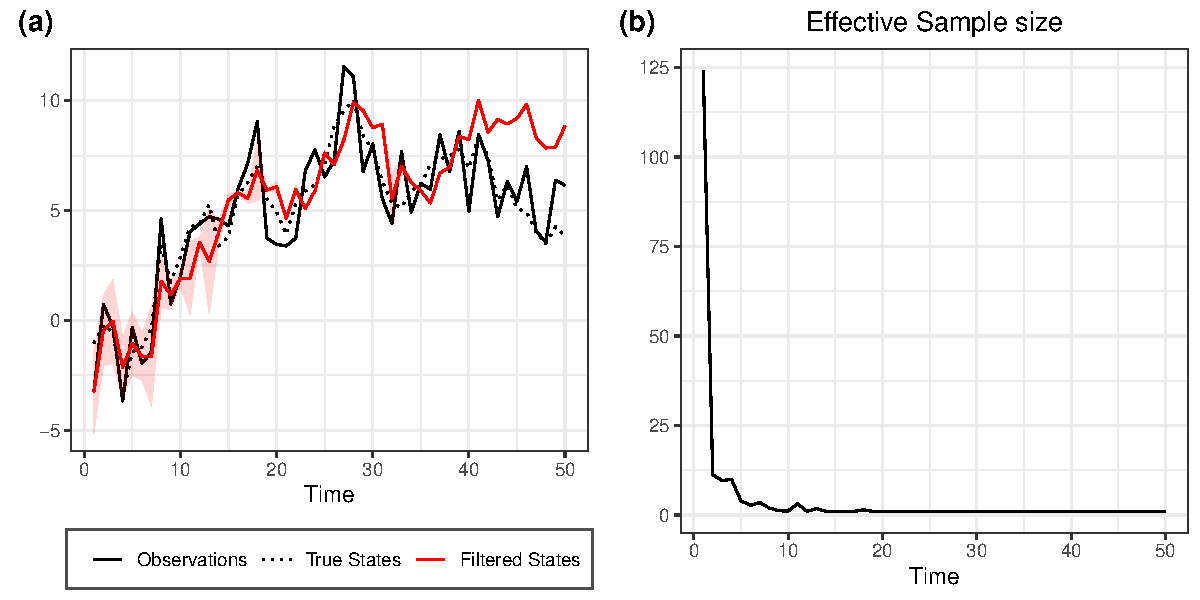
\includegraphics{prova_knit_finale_files/figure-latex/unnamed-chunk-8-1} 

}

\caption{a) SIS Filtered States with credible interval (in red). b) Effective sample size.}\label{fig:unnamed-chunk-8}
\end{figure}

\subsection{Bootstrap Particle Filter}

The bootstrap particle filter (BPF) is the easiest form of an adaptive
PF algorithm. In fact, future states are sampled from the
\textit{correct} transition kernel and the weights are updated
sequentially using the likelihood \(f_t(y_t|x_t)\).\\
We summarize the procedure with the following scheme.

\begin{enumerate}
    \item \textbf{Inital stage: }For $n=1,...,N$, at time 0 sample: $X_0^n\thicksim\mathbb P_0(dx_0)$ and set the un-normalized weights $w_0^n=1$.\
    Then, the normalized weights are: $W_0^n=\frac{1}{N}$.
    \item \textbf{For every $t=1,...T$:}
    \begin{enumerate}
        \item \textbf{Resample} if $ESS(W_{t-1}^{1:N})<ESS_{min}$:\footnote{It is indifferent to implement this resampling step at the beginning or at the end of each iteration (as we do in our codes) as long as the initial stage $t=0$ generates weights that are constant and equal to $1/N$. In fact, in this case, resampling will never take place at the beginning of the first iteration since $ESS(W_0^n=1/N)=N$ that is larger than or equal to $ESS_{min}$.\
        However, when we describe the algorithm, we chose to leave this resampling step at the beginning of each iteration. In fact, when considering the guided or auxiliary PF, we can, more generally, sample the initial values (time $t=0$) for the state from a proposal distribution different from the target one. In this case, the weights at $t=0$ might differ from $1/N$, hence resampling might take place already at the beginning of the first iteration.}
\begin{enumerate}
    \item Multinomial sampling for the indexes $(A_t^n)_n$ with probabilities given by $(W_{t-1}^n)_{n}$.
    \item Update weights as: $\hat w_{t-1}^n = 1$ for $n=1,...,N$.
\end{enumerate}
\textbf{Otherwise, } 
\begin{enumerate}
    \item Set the indexes: $A_t^{n}=n$ for $n=1,...,N$.
    \item Set the weights: $\hat w_{t-1}^n = w_{t-1}^n$ for $n=1,...,N$.
\end{enumerate}
\item Sample the future states from the transition kernel: $X_t^n\thicksim P_t(X_{t-1}^{A_t^n},dx_t)$  for $n=1,...,N$.
\item Update the un-normalized weights through the likelihood function for $n=1,...,N$.:
\begin{equation*}
    w_t^n=\hat w_{t-1}^n\cdot f_t(y_t|X_t^n).
\end{equation*}
\item Normalize the weights  for $n=1,...,N$.: $W_t^n:=\frac{w_t^n}{\sum_{m=1}^Nw_t^m}$.
    \end{enumerate}
\end{enumerate}

Therefore, at the initial step the pre-sample period states \(x_0^n\)
are extracted and every sampled state is assigned an equal weight since
there is no corresponding observation \(y_0\) that gives additional
information on the likelihood of that extraction.\\
Resampling does never take place in
\(t=1\)\footnote{Since $ESS(W_0^n=1/N)=N\geq ESS_{min}$.} and the state
in \(t=1\) is sampled from the correct transition kernel
\(P_1(x_0^n,dx_1)\). Now, the time 0 weights are updated incorporating
the information from the data point \(y_1\) in a very intuitive way:
more \textit{likely} states (given \(y_1\)) are given higher weights:
\(w_1^n=f_1(y_1|x_1^n)\). This weights are used to approximate the time
\(1\) filtering distribution.\\
At a subsequent stage, the \(ESS\) criterion should be checked and, in
case it is satisfied, resampling takes place and time \(1\) weights are
reset to be equal to \(1/N\).~\\
The key characteristic of the PF is the fact that the importance weights
are updated sequentially, according to the ``information" provided by
the observed data (i.e., the sequence \(y_{1:T}\)). Recall that time
\(t\) weight is the Radom-Nikodym derivative of the target with respect
to the proposal distribution. In the BPF, the time \(t\) target is the
measure \(\mathbb P_t(dx_{0:t}|y_{1:t})\), while the proposal, denoted
generically by \(\mathbb M_t\), is
\(\mathbb M_t(dx_{0:t}|y_{1:t})=\mathbb M_{t-1}(dx_{0:t-1}|y_{1:t-1})\cdot P_t(x_{t-1},dx_t)\).
Hence: \begin{equation}
    \begin{split}
        w_t\propto&\frac{\mathbb P_t(dx_{0:t}|y_{1:t})}{\mathbb M_t(dx_{0:t}|y_{1:t})}\propto \frac{\mathbb P_{t-1}(dx_{0:t-1}|y_{1:t-1})\cdot P_t(x_{t-1},dx_t)\cdot f(y_t|x_t)}{\mathbb M_{t-1}(dx_{0:t-1}|y_{1:t-1})\cdot P_t(x_{t-1},dx_t)}=\\
        =&\underbrace{\frac{\mathbb P_{t-1}(dx_{0:t-1}|y_{1:t-1})}{\mathbb M_{t-1}(dx_{0:t-1}|y_{1:t-1})}}_{\hat w_{t-1}}\cdot f(y_t|x_t)=\hat w_{t-1}\cdot f(y_t|x_t)
    \end{split}\label{weight_updated_bpf}
\end{equation} Finally, the BPF is able to generate the two key objects
for inference in state-space models:

\begin{itemize}
    \item the predictive distribution:
    \begin{equation}
    \begin{split}
        \mathbb P_t^N (dx_t|y_{1:t-1})=&\frac{1}{\sum_{n=1}^N\hat w_t^n}\sum_{n=1}^N\hat w_t^n\delta_{X_t^n}(dx_t)=\\
        =&\begin{cases}
        \frac{1}{N}\sum_{n=1}^N\delta_{X_t^n}(dx_t)
        ~~~~~~~~~~~~~~~~ ~\text{ if resampling occurs}\\
        \frac{1}{\sum_{n=1}^N w_{t-1}^n}\sum_{n=1}^Nw_{t-1}^n\delta_{X_t^n}(dx_t)~~~~ \text{ otherwise}
        \end{cases},
        \end{split}
    \end{equation}
    \item the filtering distribution:
    \begin{equation}
        \mathbb P_t^N (dx_t|y_{1:t})=\sum_{n=1}^NW_t^n\delta_{X_t^n}(dx_t)
    \end{equation}
\end{itemize}

\subsection{Implementation}

In this section, Bootstrap Particle Filter will be used to estimate
filtered states of the Random Walk plus Noise introduced in section
\ref{implementation}. The overall strategy replicate the SIS filter with
the addition of a ESS-based resampling step that applies when the
effective sample size is smaller than a predetermined threshold
opportunely chosen (in our example we decide to follow a common rule of
thumb consisting in setting the threshold at \(N/2\)). The steps are
presented in the following algorithm.

\begin{algorithm} BPF for Random Walk plus Noise Model
\begin{itemize}
\item Let $\{(x_{0},w_{0})^{(i)}\}_{i=1}^{N}$ summarize $p(x_{0}|y_{0})$ such that, for example, $E(g(x_{0})|y_{0}) \approx \sum_{i=1}^{N}w_{0}^{(i)}g(x_{0}^{(i)})$. In particular, initialize $(x_{0}^{(1)},...,x_{0}^{(N)})$ form $N(m_{0},C_{0})$ and set $w_{0}^{(i)}=N^{-1} \ \forall \ i=1,...,N$.
\item For $t=1,...,n$:
\begin{enumerate}
\item Draw $x_{t}^{(i)} \sim N(x_{t-1}^{(i)},\tau^2) \ \ i=1,...,N$ such that $\{(x_{t},w_{t-1})^{(i)}\}_{i=1}^{N}$ summarizes $p(x_{t}|y_{1:t-1})$
\item Set $w_{t}^{(i)} = w_{t-1}^{(i)}f_{N}(y_{t};x_{t}^{(i)},\sigma^2) \ \ i=1,...,N$ such that $\{(x_{t},w_{t})^{(i)}\}_{i=1}^{N}$ summarizes $p(x_{t}|y_{1:t})$
\item Normalize the weights: $w_{t}^{(i)}=\frac{\tilde{w}_{t}^{(i)}}{\sum_{j=1}^{N}(\tilde{w}_{t}^{(j)})}$
\item Compute $ESS=\Bigg(\sum_{i=1}^{N}(w_{t}^{(i)})^{2}\Bigg)^{-1}$
\item if $ESS<N/2$ then
\begin{enumerate}
\item Draw a sample of size N, $(x_{t}^{(1)},...,x_{t}^{(N)})$, from the discrete distribution $P(x_{t}=x_{t}^{(i)})=w_{t}^{(i)},\ \ i=1,...,N$
\item Reset the weights: $w_{t}^{(i)}=N^{-1}$, $i=1,...,N$.
\end{enumerate}
\item Set $p(x_{t}|y_{1:t})=\sum_{i=1}^{N}w_{t}^{(i)}\delta_{x_{t}^{(i)}}$
\end{enumerate}
\end{itemize}
\end{algorithm}

These steps are resumed in our \texttt{PFfun} function.\\

\hrule
\hrule

\texttt{PFfun(data,N,m0,C0,tau,sigma,r)}\\

\hrule

\textbf{Arguments}

\texttt{data} ~~the observed process. It has to be a vector or a
univariate time series.\\
\texttt{N} ~~number of particles generated at each step\\
\texttt{m0} ~~central value of the normal prior state distribution\\
\texttt{C0} ~~variance of the normal prior state distribution\\
\texttt{tau} ~~the standard deviation \(\tau\) in state equation\\
\texttt{sigma} ~~the standard deviation \(\sigma\) in observation
equation\\
\texttt{r} ~~ if present the threshold is set equal to \(N/r\)
otherwise, if missing, the threshold is set equal to \(N/2\)

\hrule
\hrule

\begin{Shaded}
\begin{Highlighting}[]
\NormalTok{PFfun<-}\ControlFlowTok{function}\NormalTok{(data,N,m0,C0,tau,sigma,r)\{}
  \ControlFlowTok{if}\NormalTok{(}\KeywordTok{missing}\NormalTok{(r))\{r=}\DecValTok{2}\NormalTok{\}}\ControlFlowTok{else}\NormalTok{\{\}}
\NormalTok{  xs<-}\OtherTok{NULL}
\NormalTok{  ws<-}\OtherTok{NULL}
\NormalTok{  ess<-}\OtherTok{NULL}
\NormalTok{  x  =}\StringTok{ }\KeywordTok{rnorm}\NormalTok{(N,m0,}\KeywordTok{sqrt}\NormalTok{(C0))}
\NormalTok{  w  =}\StringTok{ }\KeywordTok{rep}\NormalTok{(}\DecValTok{1}\OperatorTok{/}\NormalTok{N,N)}
   
  \ControlFlowTok{for}\NormalTok{(t }\ControlFlowTok{in} \DecValTok{1}\OperatorTok{:}\KeywordTok{length}\NormalTok{(data))\{}
    
\NormalTok{    x<-}\KeywordTok{rnorm}\NormalTok{(N,x,tau)}
\NormalTok{    w1<-w}\OperatorTok{*}\KeywordTok{dnorm}\NormalTok{(data[t],x,sigma)}
    
\NormalTok{    w =}\StringTok{ }\NormalTok{w1}\OperatorTok{/}\KeywordTok{sum}\NormalTok{(w1)}
\NormalTok{    ESS  =}\StringTok{ }\DecValTok{1}\OperatorTok{/}\KeywordTok{sum}\NormalTok{(w}\OperatorTok{^}\DecValTok{2}\NormalTok{)}
    
    \ControlFlowTok{if}\NormalTok{(ESS}\OperatorTok{<}\NormalTok{(N}\OperatorTok{/}\NormalTok{r))\{}
\NormalTok{      index<-}\KeywordTok{sample}\NormalTok{(N,}\DataTypeTok{size=}\NormalTok{N,}\DataTypeTok{replace=}\NormalTok{T,}\DataTypeTok{prob=}\NormalTok{w)}
\NormalTok{      x<-x[index]}
\NormalTok{      w<-}\KeywordTok{rep}\NormalTok{(}\DecValTok{1}\OperatorTok{/}\NormalTok{N,N)}
\NormalTok{    \}}\ControlFlowTok{else}\NormalTok{\{\}}
    
\NormalTok{    xs =}\StringTok{ }\KeywordTok{rbind}\NormalTok{(xs,x)}
\NormalTok{    ws =}\StringTok{ }\KeywordTok{rbind}\NormalTok{(ws,w)}
\NormalTok{    ess =}\KeywordTok{rbind}\NormalTok{(ess,ESS)}
\NormalTok{  \}}
  \KeywordTok{return}\NormalTok{(}\KeywordTok{list}\NormalTok{(}\DataTypeTok{xs=}\NormalTok{xs,}\DataTypeTok{ws=}\NormalTok{ws,}\DataTypeTok{ess=}\NormalTok{ess))}
\NormalTok{\}}
\end{Highlighting}
\end{Shaded}

The estimated states of the Boostrap Particle Filter togheter with the
effective sample size are shown in Figure \ref{fig:myfig3}. We decide to
set \(N=1000\), \(m_{0}=0\), \(C_{0}=100\) and \(\tau=\sigma=1\). Notice
how the resampling step allows the effective sample size not to drop,
improving results.

\begin{figure}[H]

{\centering 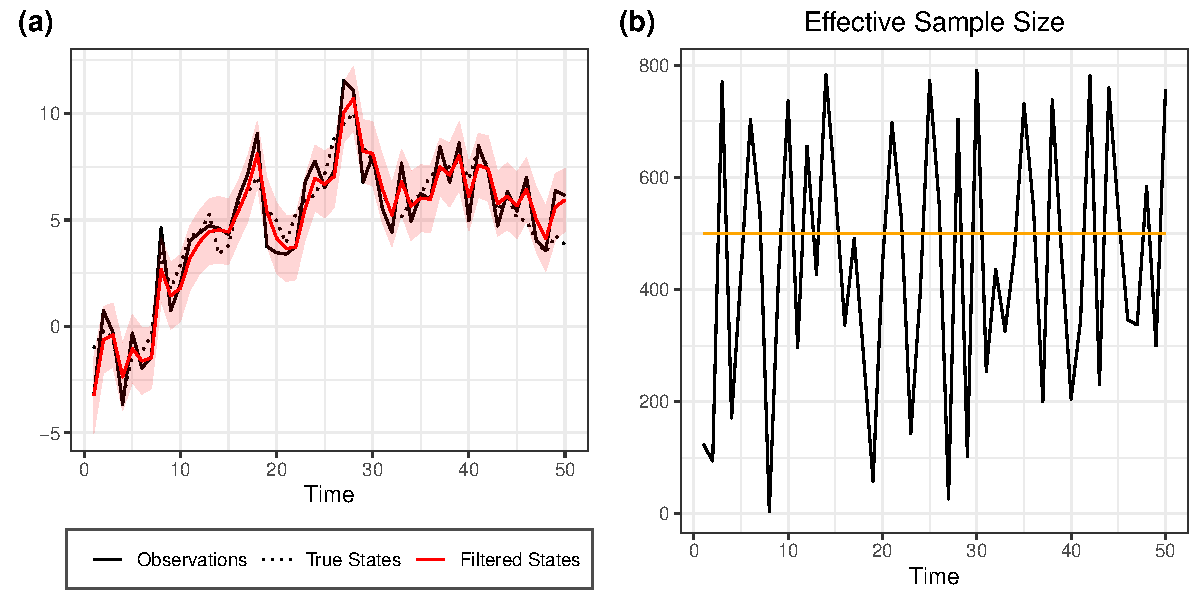
\includegraphics{prova_knit_finale_files/figure-latex/myfig3-1} 

}

\caption{a) PF Filtered States with credible interval (in red). b) Effective sample size (in black) with threshold (in yellow).}\label{fig:myfig3}
\end{figure}

Since the Random Walk plus Noise model allows for closed form solutions,
we want to compare the results of Boostrap Particle Filter(BPF) with
Kalman Filter(KF). As we can see from figure \ref{fig:myfig4}, as the
number of particles N increases, both the state level and the standard
deviation estimated with particle filter converge to the ones obtained
by the recursive Kalman filter formulas, confirming Monte Carlo
approximations to be asymptotically consistent. Moreover, comparing the
Root Mean Square Errors of the filtered states with respect to the true
state values, when the sample size increases the BPF decreases and, for
large N, it reaches the accuracy of the Kalman Filter.

\begin{longtable}[t]{cccc}
\caption{\label{tab:unnamed-chunk-12}Root Mean Square Errors}\\
\toprule
N & Threshold & KF & BPF\\
\midrule
100 & 0.5 & 0.879 & 0.916\\
1000 & 0.5 & 0.879 & 0.882\\
10000 & 0.5 & 0.879 & 0.885\\
\bottomrule
\end{longtable}

\begin{figure}[H]

{\centering 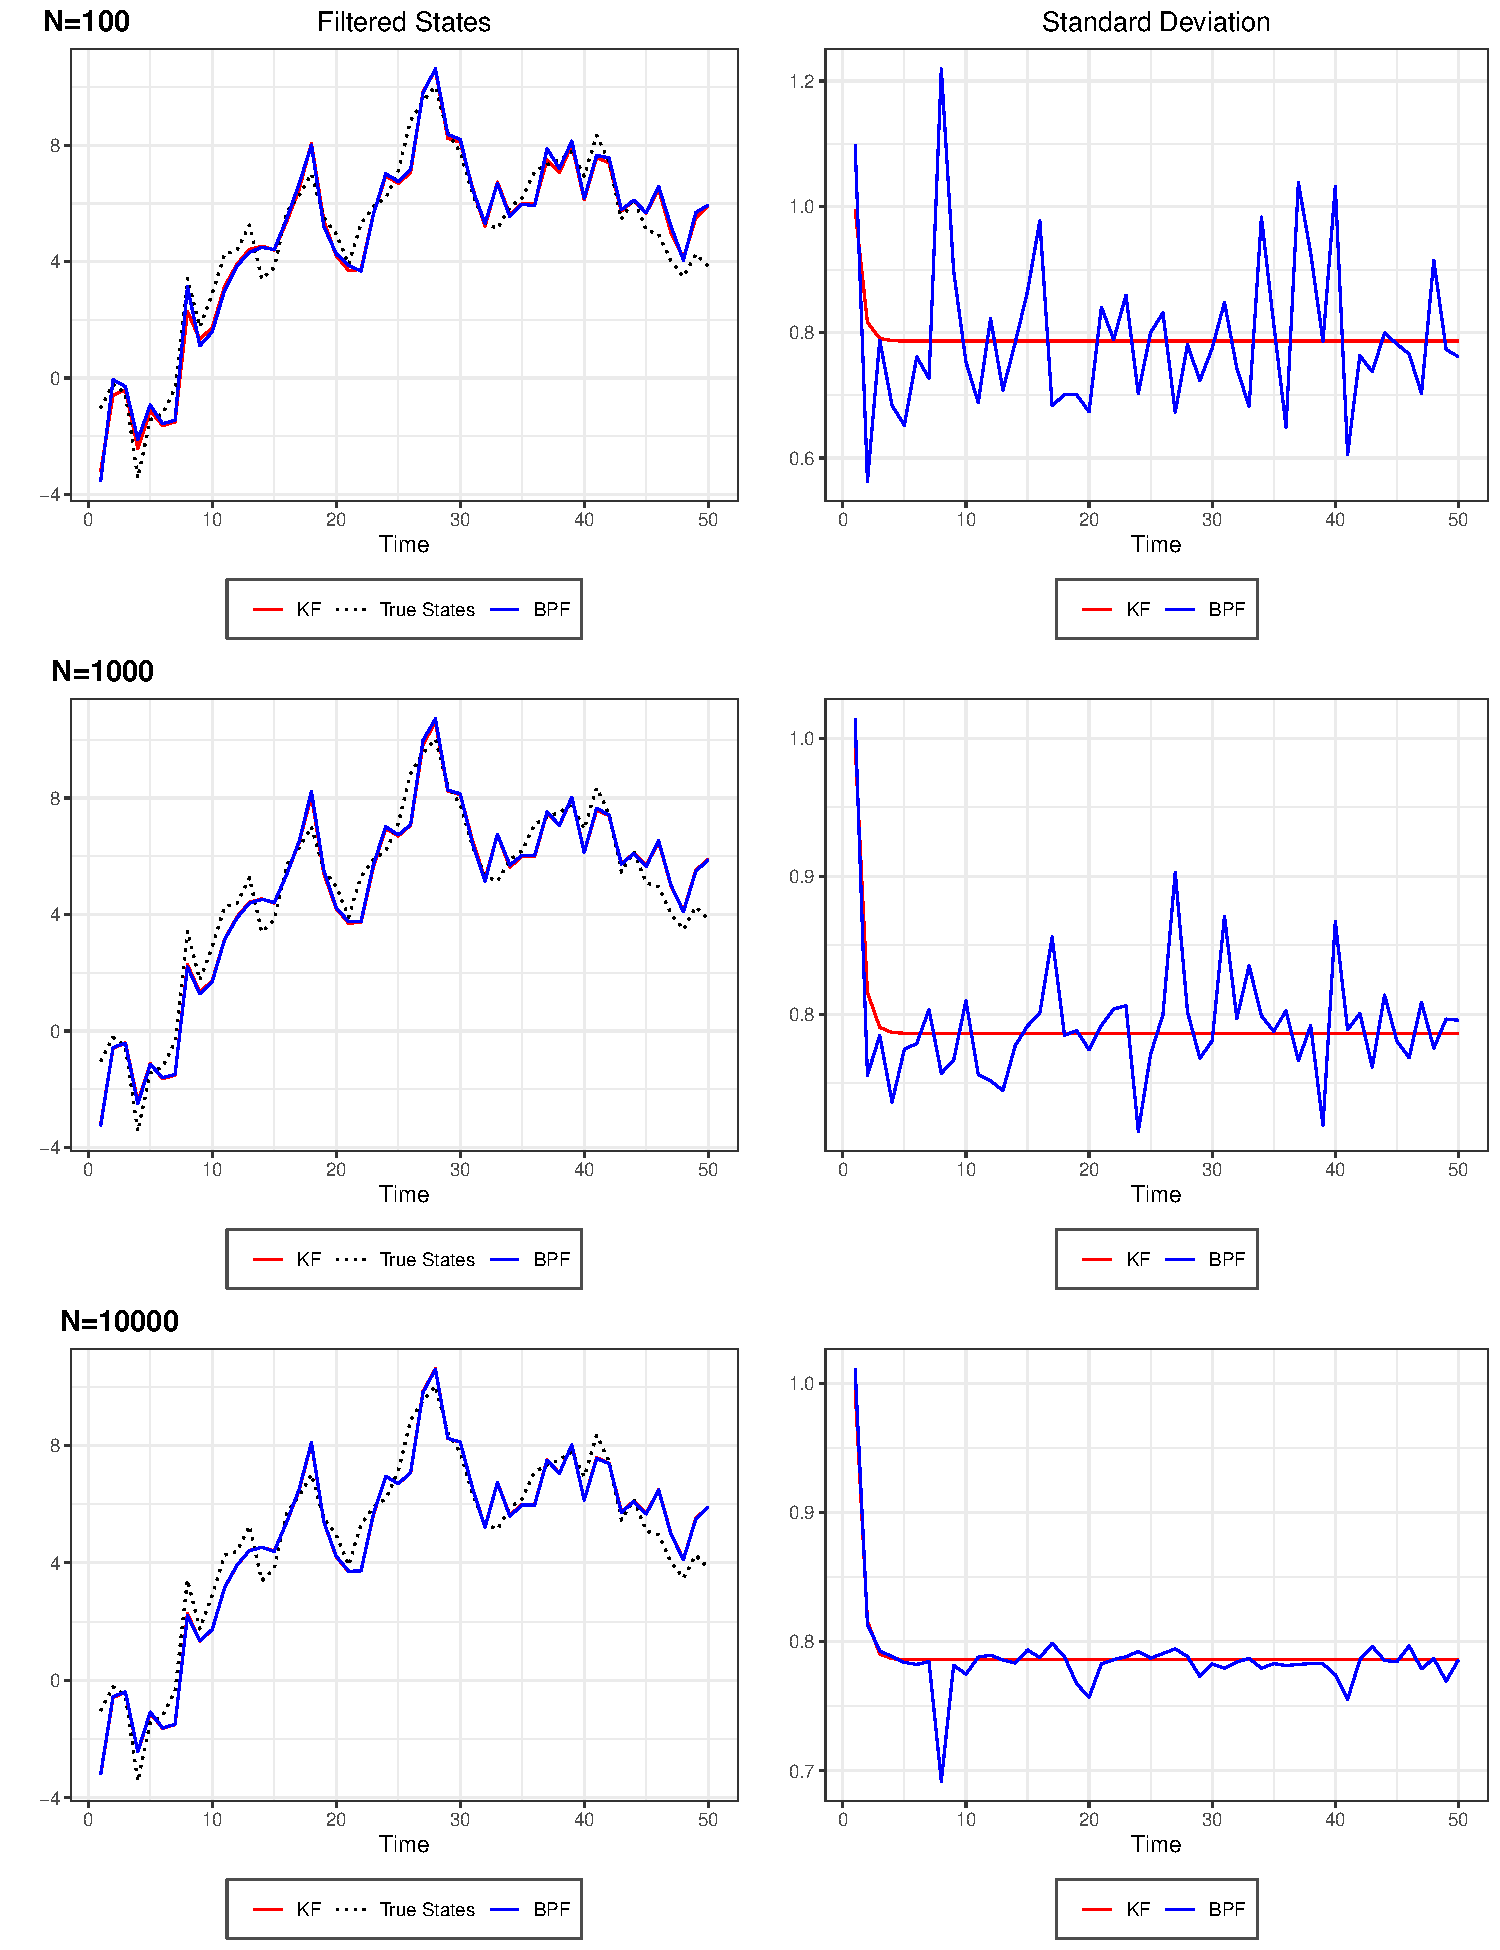
\includegraphics{prova_knit_finale_files/figure-latex/myfig4-1} 

}

\caption{Comparison Bootstrap Particle Filter(BPF) and Kalman Filter (KF) for increasing number of generated particles (N)}\label{fig:myfig4}
\end{figure}

\subsection{Guided Particle Filter}

It is not always possible to sample sequentially from the correct
transition kernel. Moreover, even if it were possible, there exist a
proposal transition kernel that makes the algorithm more efficient. This
motivates the \textit{guided particle filter} (GPF), that can be
interpreted as a more general version of the BPF. In fact, with the GPF
it is possible, at each stage, to sample new states from a transition
kernel that differs from the correct one.~\\
Let \(P_t(x_{t-1},dx_t)\) be the correct kernel and consider a kernel
\(M_t(x_{t-1},dx_t)\) defined on the same measurable space of \(P_t\).
Moreover, let us assume that that \(P_t\) is absolutely continuous with
respect to
\(M_t\)\footnote{This condition is stronger than what would be needed for the existence of the importance weights in GPF, i.e., that  $P_t(x_{t-1},dx_t)\cdot f_t(y_t|x_t)\ll M_t(x_{t-1},dx_t)$. }
(i.e., \(P_t\ll M_t\)). If sampling occurs sequentially from this
kernel, the way in which weights are updated should differ from the BPF.
Consider equation \eqref{weight_updated_bpf} and let us reformulate it
for the GPF case. Here, the proposal distribution is not
\(\mathbb M_t(dx_{0:t}|y_{1:t})=\mathbb M_{t-1}(dx_{0:t-1}|y_{1:t-1})\cdot P_t(x_{t-1},dx_t)\)
anymore, but becomes
\(\mathbb M_t(dx_{0:t}|y_{1:t})=\mathbb M_{t-1}(dx_{0:t-1}|y_{1:t-1})\cdot M_t(x_{t-1},dx_t)\).
Hence: \begin{equation}
    \begin{split}
        w_t\propto&\frac{\mathbb P_t(dx_{0:t}|y_{1:t})}{\mathbb M_t(dx_{0:t}|y_{1:t})}\propto \frac{\mathbb P_{t-1}(dx_{0:t-1}|y_{1:t-1})\cdot P_t(x_{t-1},dx_t)\cdot f_t(y_t|x_t)}{\mathbb M_{t-1}(dx_{0:t-1}|y_{1:t-1})\cdot M_t(x_{t-1},dx_t)}=\\
        =&\underbrace{\frac{\mathbb P_{t-1}(dx_{0:t-1}|y_{0:t-1})}{\mathbb M_{t-1}(dx_{0:t-1}|y_{1:t-1})}}_{\hat w_{t-1}}\cdot\frac{P_t(x_{t-1},dx_t)\cdot f_t(y_t|x_t)}{ M_t(x_{t-1},dx_t)} =\hat w_{t-1}\cdot\underbrace{\frac{P_t(x_{t-1},dx_t)\cdot f_t(y_t|x_t)}{ M_t(x_{t-1},dx_t)}}_{\text{updating factor}}
    \end{split}\label{weight_updated_gpf}
\end{equation} Note that the updating factor is more complex that the
one of the BPF: in addition to the likelihood function \(f_t(y_t|x_t)\),
the fact that sampling occurs from a kernel different from the correct
ones requires the additional term
\(P_t(x_{t-1},dx_t)/M_t(x_{t-1},dx_t)\).~\\
We are now ready to establish, informally, the optimality result about
the transition kernel. Let us denote by
\(G_t=[P_t(x_{t-1},dx_t)\cdot f_t(y_t|x_t)dy_t]/M_t(x_{t-1},dx_t)\) the
\textit{incremental weights} (i.e., the updating factor) and by
\(M_t^*(x_{t-1},dx_t)\) the optimal kernel. It can be
proved\footnote{For a formal proof see Chopin and Papaspiliopoulos (2020), th. 10.1 p. 142.}
that the optimal kernel, i.e., the one that minimizes the variance of
the incremental weights \(G_t\) (and of the time \(t\) weights
themselves), is: \begin{equation}
    M_t^*(x_{t-1},dx_t)=\frac{1}{\int_{\mathcal X}P_t(x_{t-1},dx_t)\cdot f_t(y_t|x_t)} P_t(x_{t-1},dx_t)\cdot f_t(y_t|x_t)
\end{equation} Note that \(M_t^*\) is the conditional distribution of
\(x_t\) given \(x_{t-1}\) and
\(y_t\).\footnote{In fact, assuming that the $P_t$ admits a density $p_t$, applying Bayes rule, we have that $m_t(x_t|x_{t-1},y_t)\propto p_t(x_t|x_{t-1})\cdot f(y_t|x_t)$.}
The intuition for this result is apparent when considering equation
\eqref{weight_updated_gpf}: if \(M_t=M_t^*\), the updating factor
collapses to \(\int_{\mathcal X}P_t(x_{t-1},dx_t)\cdot f_t(y_t|x_t)\)
and information from the observed data are incorporated efficiently.\\
As a matter of fact, it is usually impossible to sample from the optimal
kernel and, in practice, it is replaced by its linear Gaussian
approximation. ~\\
The GPF can be resumed by the following steps.

\begin{enumerate}
    \item \textbf{Inital stage: }For $n=1,...,N$, at time 0 sample: $X_0^n\thicksim\mathbb M_0(dx_0)$ and set the un-normalized weights: 
    $$w_0^n=\frac{\mathbb P_0(dx_0)}{\mathbb M_0(dx_0)}.$$
    Then, the normalized weights are: $W_0^n:=\frac{w_0^n}{\sum_{m=1}^Nw_0^m}$.
    \item \textbf{For every $t=1,...T$:}
    \begin{enumerate}
        \item \textbf{Resample} if $ESS(W_{t-1}^{1:N})<ESS_{min}$:
\begin{enumerate}
    \item Multinomial sampling for the indexes $(A_t^n)_n$ with probabilities given by $(W_{t-1}^n)_n$.
    \item Update weights as: $\hat w_{t-1}^n = 1$ for $n=1,...,N$.
\end{enumerate}
\textbf{Otherwise, } 
\begin{enumerate}
    \item Set the indexes: $A_t^{n}=n$ for $n=1,...,N$
    \item Set the weights: $\hat w_{t-1}^n = w_{t-1}$ for $n=1,...,N$.
\end{enumerate}
\item Sample the future states from the transition kernel: $X_t^n\thicksim M_t(X_{t-1}^{A_t^n},dx_t)$ for $n=1,...,N$.
\item Update the un-normalized weights, for $n=1,...,N$:
\begin{equation*}
    w_t^n=\hat w_{t-1}^n\cdot \frac{P_t(X_{t-1}^{A_t^n},dx_t)\cdot f_t(y_t|X_t^n)}{ M_t(X_{t-1}^{A_t^n},dx_t)}.
\end{equation*}
\item Normalize the weights, for $n=1,...,N$:  $W_t^n:=\frac{w_t^n}{\sum_{m=1}^Nw_t^m}$.
    \end{enumerate}
\end{enumerate}

Note that \(\mathbb M_0(dx_0)\) is the initial sampling distribution,
that could differ from the correct one \(\mathbb P_0(dx_0)\).~\\
To conclude, one of the issues related to the BPF is the fact that new
states in \(t\) are sampled ignoring their likelihood given the future
observation \(y_t\). Hence, extractions from the ``correct" transition
kernel may be associated to low weights (small value for the
likelihood). Instead, the GPF allows to solve for this problem, defining
a proposal kernel that depends on the likelihood itself. Therefore, the
extraction of future states already incorporates the information given
by the data resulting in a more efficient procedure.

\subsection{Implementation}

The Bootstrap Particle Filter Approach for the Random Walk plus Noise
Model described in Section \ref{implementation} can be improved
accounting for the observations in the importance transition density and
it consists of generating \(x_{t}\) from its conditional distribution
given \(x_{t-1}\) and \(y_{t}\). In the Normal model we are considering,
the optimal proposal will be a Normal density as well with mean and
variance given by \begin{align*}
\mu_{opt}=E(x_{t}|x_{t-1},y_{t})&=x_{t-1}+\frac{\tau^{2}}{\tau^{2}+\sigma^{2}}(y_{t}-x_{t-1})\\
\sigma_{opt}^{2}=V(x_{t}|x_{t-1},y_{t})&=\frac{\tau^{2}\sigma^{2}}{\tau^{2}+\sigma^{2}}
\end{align*} On the other hand, the incremental weights, using this
importance transition density, are proportional to the conditional
density of \(y_{t}\) given \(x_{t-1}=x_{t-1}^{(i)}\) , i.e
\(N(x_{t-1}^{(i)},\tau^{2}+\sigma^{2})\), evaluated at \(y_{t}\). In
other words the algorithm implemented in R is:

\begin{algorithm} GPF for Random Walk plus Noise Model
\begin{itemize}
\item Let $\{(x_{0},w_{0})^{(i)}\}_{i=1}^{N}$ summarize $p(x_{0}|y_{0})$ such that, for example, $E(g(x_{0})|y_{0}) \approx \sum_{i=1}^{N}w_{0}^{(i)}g(x_{0}^{(i)})$. In particular, initialize $(x_{0}^{(1)},...,x_{0}^{(N)})$ from $N(m_{0},C_{0})$ and set $w_{0}^{(i)}=N^{-1} \ \forall \ i=1,...,N$.
\item Compute $\sigma_{opt}^{2}$ 
\item For $t=1,...,n$:
\begin{enumerate}
\item Compute $\mu_{opt}$
\item Draw $x_{t}^{(i)} \sim N(\mu_{opt},\sigma_{opt}^{2}) \ \ i=1,...,N$ such that $\{(x_{t},w_{t-1})^{(i)}\}_{i=1}^{N}$ summarizes $p(x_{t}|y_{1:t-1})$
\item Set $w_{t}^{(i)} = w_{t-1}^{(i)}f_{N}(y_{t};x_{t}^{(i)},\sigma^2+\tau^{2}) \ \ i=1,...,N$ such that $\{(x_{t},w_{t})^{(i)}\}_{i=1}^{N}$ summarizes $p(x_{t}|y_{1:t})$
\item Normalize the weights: $w_{t}^{(i)}=\frac{\tilde{w}_{t}^{(i)}}{\sum_{j=1}^{N}(\tilde{w}_{t}^{(j)})}$
\item Compute $ESS=\Bigg(\sum_{i=1}^{N}(w_{t}^{(i)})^{2}\Bigg)^{-1}$
\item if $ESS<N/2$ then
\begin{enumerate}
\item Draw a sample of size N, $(x_{t}^{(1)},...,x_{t}^{(N)})$, from the discrete distribution $P(x_{t}=x_{t}^{(i)})=w_{t}^{(i)},\ \ i=1,...,N$
\item Reset the weights: $w_{t}^{(i)}=N^{-1}$, $i=1,...,N$.
\end{enumerate}
\item Set $p(x_{t}|y_{1:t})=\sum_{i=1}^{N}w_{t}^{(i)}\delta_{x_{t}^{(i)}}$
\end{enumerate}
\end{itemize}
\end{algorithm}

The \texttt{GPFfun} function resume this passages.\\

\hrule
\hrule

\texttt{GPFfun(data,N,m0,C0,tau,sigma,r)}\\

\hrule

\textbf{Arguments}

\texttt{data} ~~the observed process. It has to be a vector or a
univariate time series.\\
\texttt{N} ~~number of particles generated at each step\\
\texttt{m0} ~~central value of the normal prior state distribution\\
\texttt{C0} ~~variance of the normal prior state distribution\\
\texttt{tau} ~~the standard deviation \(\tau\) in state equation\\
\texttt{sigma} ~~the standard deviation \(\sigma\) in observation
equation\\
\texttt{r} ~~ if present the threshold is set equal to \(N/r\)
otherwise, if missing, the threshold is set equal to \(N/2\)

\hrule
\hrule

\begin{Shaded}
\begin{Highlighting}[]
\NormalTok{GPFfun<-}\ControlFlowTok{function}\NormalTok{(data,N,m0,C0,tau,sigma,r)\{}
  \ControlFlowTok{if}\NormalTok{(}\KeywordTok{missing}\NormalTok{(r))\{r=}\DecValTok{2}\NormalTok{\}}\ControlFlowTok{else}\NormalTok{\{\}}
\NormalTok{  xs<-}\OtherTok{NULL}
\NormalTok{  ws<-}\OtherTok{NULL}
\NormalTok{  ess<-}\OtherTok{NULL}
\NormalTok{  x  =}\StringTok{ }\KeywordTok{rnorm}\NormalTok{(N,m0,}\KeywordTok{sqrt}\NormalTok{(C0))}
\NormalTok{  importancesd<-}\KeywordTok{sqrt}\NormalTok{(tau }\OperatorTok{-}\StringTok{ }\NormalTok{tau}\OperatorTok{^}\DecValTok{2} \OperatorTok{/}\NormalTok{(tau }\OperatorTok{+}\StringTok{ }\NormalTok{sigma))}
\NormalTok{  predsd <-}\StringTok{ }\KeywordTok{sqrt}\NormalTok{(sigma}\OperatorTok{+}\NormalTok{tau)}
\NormalTok{  w  =}\StringTok{ }\KeywordTok{rep}\NormalTok{(}\DecValTok{1}\OperatorTok{/}\NormalTok{N,N)}
  
  \ControlFlowTok{for}\NormalTok{(t }\ControlFlowTok{in} \DecValTok{1}\OperatorTok{:}\KeywordTok{length}\NormalTok{(data))\{}
    
\NormalTok{    means<-x}\OperatorTok{+}\NormalTok{(tau}\OperatorTok{/}\NormalTok{(tau}\OperatorTok{+}\NormalTok{sigma))}\OperatorTok{*}\NormalTok{(data[t]}\OperatorTok{-}\NormalTok{x)}
\NormalTok{    x<-}\KeywordTok{rnorm}\NormalTok{(N,means,importancesd)}
\NormalTok{    w1<-w}\OperatorTok{*}\KeywordTok{dnorm}\NormalTok{(data[t],x,predsd)}
    
\NormalTok{    w =}\StringTok{ }\NormalTok{w1}\OperatorTok{/}\KeywordTok{sum}\NormalTok{(w1)}
\NormalTok{    ESS  =}\StringTok{ }\DecValTok{1}\OperatorTok{/}\KeywordTok{sum}\NormalTok{(w}\OperatorTok{^}\DecValTok{2}\NormalTok{)}
    
    \ControlFlowTok{if}\NormalTok{(ESS}\OperatorTok{<}\NormalTok{(N}\OperatorTok{/}\NormalTok{r))\{}
\NormalTok{      index<-}\KeywordTok{sample}\NormalTok{(N,}\DataTypeTok{size=}\NormalTok{N,}\DataTypeTok{replace=}\NormalTok{T,}\DataTypeTok{prob=}\NormalTok{w)}
\NormalTok{      x<-x[index]}
\NormalTok{      w<-}\KeywordTok{rep}\NormalTok{(}\DecValTok{1}\OperatorTok{/}\NormalTok{N,N)}
\NormalTok{    \}}\ControlFlowTok{else}\NormalTok{\{\}}
    
\NormalTok{    xs =}\StringTok{ }\KeywordTok{rbind}\NormalTok{(xs,x)}
\NormalTok{    ws =}\StringTok{ }\KeywordTok{rbind}\NormalTok{(ws,w)}
\NormalTok{    ess =}\KeywordTok{rbind}\NormalTok{(ess,ESS)}
\NormalTok{  \}}
  \KeywordTok{return}\NormalTok{(}\KeywordTok{list}\NormalTok{(}\DataTypeTok{xs=}\NormalTok{xs,}\DataTypeTok{ws=}\NormalTok{ws,}\DataTypeTok{ess=}\NormalTok{ess))}
\NormalTok{\}}
\end{Highlighting}
\end{Shaded}

\begin{figure}[H]

{\centering 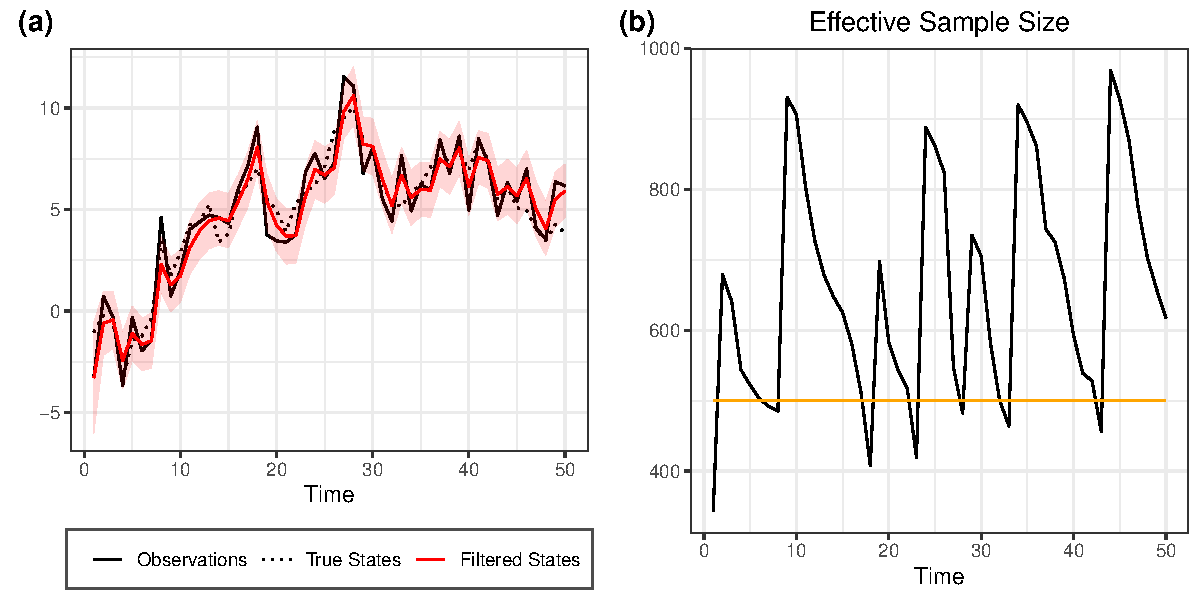
\includegraphics{prova_knit_finale_files/figure-latex/unnamed-chunk-15-1} 

}

\caption{a) GPF Filtered States with credible interval (in red). b) Effective sample size (in black) with threshold (in yellow).}\label{fig:unnamed-chunk-15}
\end{figure}

Let's provide directly a brief comparison between the Bootstrap Particle
Filter (BPF) and the Guided Particle Filter (GPF). As we can see from
the Figure \ref{fig:myfig5}, the Guided Particle Filter provides point
estimates that are slightly better with respect to the ones of the BPF,
and this is confirmed by the Table showing the RMSE. Moreover, the
variance is lower, suggesting for higher precision.

\begin{longtable}[t]{cccc}
\caption{\label{tab:unnamed-chunk-17}Root Mean Square Errors}\\
\toprule
N & Threshold & BPF & GPF\\
\midrule
1000 & 0.50 & 0.882 & 0.874\\
1000 & 0.25 & 0.889 & 0.874\\
1000 & 0.10 & 0.885 & 0.879\\
\bottomrule
\end{longtable}

\begin{figure}[H]

{\centering 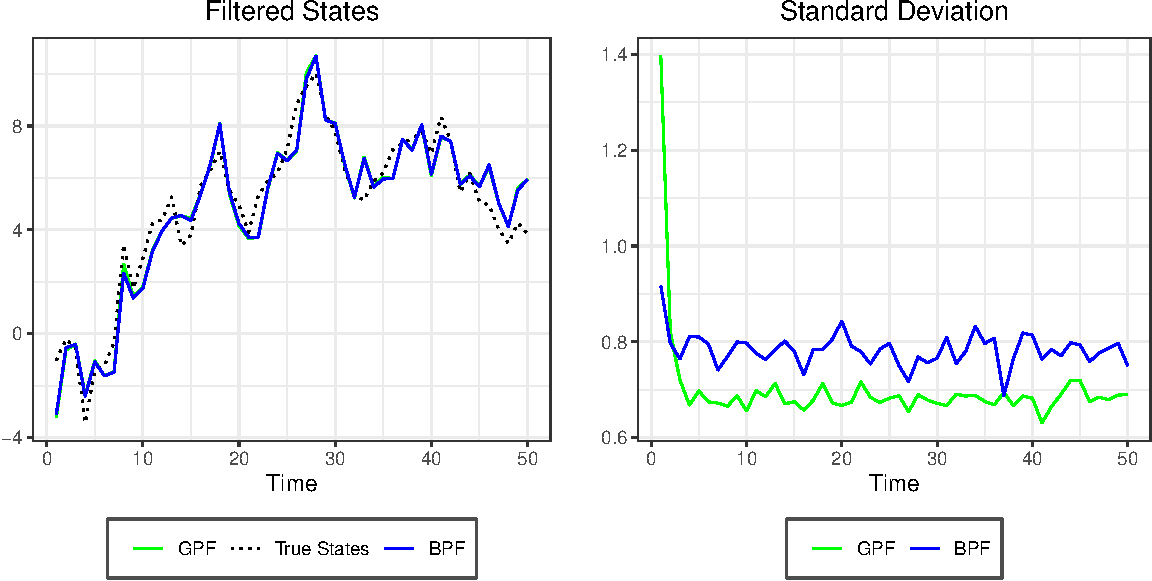
\includegraphics{prova_knit_finale_files/figure-latex/myfig5-1} 

}

\caption{Comparison Bootstrap Particle Filter(BPF) and Guided Particle Filter (GPF), number of generated particles N=1000}\label{fig:myfig5}
\end{figure}

\subsection{Auxiliary Particle Filter}

The \textit{auxiliary particle filter} (APF) constitutes a further
extension of the BPF. The GPF allowed to sample from a transition kernel
different from the correct ones. The APF, instead, allows to extract the
ancestor variables from an arbitrary distribution at the resampling
step.~\\
Let \(\eta_t:\mathcal X\rightarrow \mathbb R_+\) be a non-negative,
real-valued positive function, called \textit{auxiliary function}. At
time \(t\), when the resampling stage occurs, the multinomial
distribution for the indexes to be extracted can use probabilities that
differ from the weights in \(t-1\), \(W_{t-1}^n\). The new weights,
called \textit{auxiliary weights}, are computed as a transformation of
the original ones, denoted as \textit{inferential weights}, through the
auxiliary function: \begin{equation}
    \tilde W_t^n=\frac{W_t^n\cdot \eta_t(X_t^n)}{\sum_{m=1}^NW_t^m\cdot \eta_t(X_t^n)}
\end{equation} Note that the computation of the auxiliary weights is
done from the auto-normalized inferential ones. Additionally, note that
imposing \(\eta_t(x_t)=1\) we recover the GPF and the BPF as special
cases of the APF.\\
Clearly, inferential weights are updated by incorporating the fact that
resampling occurs according to different weights (the auxiliary ones):
\begin{equation}
    w_t^n=\frac{W_{t-1}^{A_t^n}}{\tilde W_{t-1}^{A_t^n}}G_t \label{apf_weights_up_}
\end{equation} where \(G_t\) is the incremental weight defined in the
section on GPF.~\\

To understand the logic of this sequential weight updating, consider
\eqref{weight_updated_gpf}. In particular, suppose that multinomial
resampling takes place at every stage and let
\(\tilde w_{t-1}:=w_{t-1}\cdot \eta_{t-1} (x_{t-1})\). Then:
\begin{equation}
    \begin{split}
        w_t\propto&\frac{\mathbb P_t(dx_{0:t}|y_{1:t})}{\mathbb M_t(dx_{0:t}|y_{1:t})}\propto \frac{\mathbb P_{t-1}(dx_{0:t-1}|y_{0:t-1})}{\mathbb M_{t-1}(dx_{0:t-1}|y_{1:t-1})\cdot \tilde w_{t-1}}\cdot\frac{P_t(x_{t-1},dx_t)\cdot f_t(y_t|x_t)}{ M_t(x_{t-1},dx_t)}\\
        =&\underbrace{\frac{\mathbb P_{t-1}(dx_{0:t-1}|y_{0:t-1})}{\mathbb M_{t-1}(dx_{0:t-1}|y_{1:t-1})}}_{w_{t-1}}\cdot\frac{1}{\tilde w_{t-1}}\cdot\frac{P_t(x_{t-1},dx_t)\cdot f_t(y_t|x_t)}{ M_t(x_{t-1},dx_t)}\\
        =&\frac{w_{t-1}}{ \tilde w_{t-1}}\cdot\frac{P_t(x_{t-1},dx_t)\cdot f_t(y_t|x_t)}{ M_t(x_{t-1},dx_t)}\label{weight_updated_apf}
    \end{split}
\end{equation} It is possible to derive an optimality result for the
auxiliary
functions\footnote{Details in Chopin and Papaspiliopoulos (2020) th 10.2, p. 148}.
In the special case in which the transition kernel used for sampling
corresponds with the optimal one \(M_t^*\), the optimal auxiliary
function (i.e., the auxiliary function that minimizes the variance of
the inferential weights) becomes: \begin{equation}
    \eta_{t-1}^*(x_{t-1})=\int_\mathcal XP_t(x_{t-1},dx_t)f_t(y_t|x_t)
\end{equation} and is called \textit{perfectly adapted} auxiliary
function. In fact, if \(M_t=M_t^*\), then, expression
\eqref{weight_updated_apf} becomes: \begin{equation*}
    \begin{split}
        w_t\propto\frac{w_{t-1}}{ \tilde w_{t-1}}\cdot\frac{P_t(x_{t-1},dx_t)\cdot f_t(y_t|x_t)}{ M_t^*(x_{t-1},dx_t)}=\frac{1}{\eta_{t-1} (x_{t-1})}\cdot\int_\mathcal XP_t(x_{t-1},dx_t)f_t(y_t|x_t)
    \end{split}
\end{equation*} From the previous equation, it is clear that if
\(\eta_t=\eta_t^*\), the inferential weights are constant and their
variance is zero.\\
We can summarize the APF algorithm.

\begin{enumerate}
    \item \textbf{Inital stage: }
    \begin{enumerate}
        \item For $n=1,...,N$, at time 0 sample: $X_0^n\thicksim\mathbb M_0(dx_0)$ and set the un-normalized inferential weights: 
    $$w_0^n=\frac{\mathbb P_0(dx_0)}{\mathbb M_0(dx_0)}.$$
    Then, the normalized inferential weights are: $W_0^n:=\frac{w_0^n}{\sum_{m=1}^Nw_0^m}$.
    \item Compute the un-normalized auxiliary weights:
        $$\tilde w_0^n=w_0^n \cdot \eta_0(X_0^n)$$
        Then the normalized auxiliary weights are:
        $\tilde W_0^n:=\frac{\tilde w_0^n}{\sum_{m=1}^N\tilde w_0^m}$.
    \end{enumerate}
    \item \textbf{For every $t=1,...T$:}
    \begin{enumerate}
        \item \textbf{Resample} if $ESS( W_{t-1}^{1:N})<ESS_{min}$:
\begin{enumerate}
    \item Multinomial sampling for the indexes $(A_t^n)_n$ with probabilities given by $(\tilde W_{t-1}^n)_n$.
    \item Update weights as: $\hat w_{t-1}^n = \frac{W_{t-1}^{A_t^n}}{\tilde W_{t-1}^{A_t^n}} $ for $n=1,...,N$.
\end{enumerate}
\textbf{Otherwise, } 
\begin{enumerate}
    \item Set the indexes: $A_t^{n}=n$ for  $n=1,...,N$.
    \item Set the weights: $\hat w_{t-1}^n = w_{t-1}$ for $n=1,...,N$.
\end{enumerate}
\item Sample the future states from the transition kernel: $X_t^n\thicksim M_t(X_{t-1}^{A_t^n},dx_t)$ for $n=1,...,N$.
\item Update the un-normalized inferential weights, for $n=1,...,N$:
\begin{equation*}
    w_t^n=\hat w_{t-1}^n\cdot \frac{P_t(X_{t-1}^{A_t^n},dx_t)\cdot f_t(y_t|X_t^n)}{ M_t(X_{t-1}^{A_t^n},dx_t)}.
\end{equation*}
\item Normalize the inferential weights, for $n=1,...,N$:  $W_t^n:=\frac{w_t^n}{\sum_{m=1}^Nw_t^m}$.
\item Compute the un-normalized auxiliary weights, for $n=1,...,N$:
\begin{equation*}
 \tilde w_t^n=w_t^n \cdot \eta_t(X_t^n)
\end{equation*}
\item Normalize the auxiliary weights, for $n=1,...,N$:  $\tilde W_t^n:=\frac{\tilde w_t^n}{\sum_{m=1}^N\tilde w_t^m}$.\footnote{It is worth mentioning that the original APF included a final resampling step at the end of each iteration. However, our formulation is more efficient since having two resampling steps might introduce additional Monte Carlo variance. See Johansen and Evers (2007), p. 120}
    \end{enumerate}
\end{enumerate}

However, it is worth noting that the optimality results both for the
kernel in the GPF and of the auxiliary in the APF, has two main
weaknesses:

\begin{itemize}
    \item it is not clear that what is optimal at time $t$ remains such at future stages. In other words, it is not truly clear how the minimization of the variance of the inferential weights at each stage affects the efficiency of the PF estimators;
    \item both the choice of $M_t$ and of $\eta_t$ affect the way in which weights are computed and, indirectly, the decision to resample in the future. It is difficult to take also this indirect effect into account when evaluating the  overall efficiency of the algorithm.
\end{itemize}

\subsection{Implementation}

For illustration purposes, we are going implement an auxiliary particle
filter for the linear Gaussian model with auxiliary function
\(g(x_{t-1})=E(x_{t}|x_{t-1})=x_{t-1}\).

\begin{algorithm} APF for Random Walk plus Noise Model
\begin{itemize}
\item Let $\{(x_{0},w_{0})^{(i)}\}_{i=1}^{N}$ summarize $p(x_{0}|y_{0})$ such that, for example, $E(g(x_{0})|y_{0}) \approx \sum_{i=1}^{N}w_{0}^{(i)}g(x_{0}^{(i)})$. In particular, initialize $(x_{0}^{(1)},...,x_{0}^{(N)})$ from $N(m_{0},C_{0})$ and set $w_{0}^{(i)}=N^{-1} \ \forall \ i=1,...,N$.
\item For $t=1,...,n$:
\begin{enumerate}
\item For $k=1,...,N$:
\begin{enumerate}
\item Draw $I_{k}$ with $P(I_{k}=i) \propto w_{t-1}^{(i)}f(y_{t}|g(x_{t-1}^{(i)})) $
\item Draw $x_{t}^{(k)} \sim N(x_{t-1}^{(I_{k})},\tau^2)$
\item Set  $\tilde{w}_{t}^{(k)} = \frac{f_{N}(y_{t}|x_{t}^{(k)})}{f_{N}(y_{t}|g(x_{t-1}^{(I_{k})}))}$
\end{enumerate}
\item Normalize the weights: $w_{t}^{(i)}=\frac{\tilde{w}_{t}^{(i)}}{\sum_{j=1}^{N}(\tilde{w}_{t}^{(j)})}$
\item Compute $ESS=\Bigg(\sum_{i=1}^{N}(w_{t}^{(i)})^{2}\Bigg)^{-1}$
\item if $ESS<N/2$ then
\begin{enumerate}
\item Draw a sample of size N, $(x_{t}^{(1)},...,x_{t}^{(N)})$, from the discrete distribution $P(x_{t}=x_{t}^{(i)})=w_{t}^{(i)},\ \ i=1,...,N$
\item Reset the weights: $w_{t}^{(i)}=N^{-1}$, $i=1,...,N$.
\end{enumerate}
\item Set $p(x_{t}|y_{1:t})=\sum_{i=1}^{N}w_{t}^{(i)}\delta_{x_{t}^{(i)}}$
\end{enumerate}
\end{itemize}
\end{algorithm}

The \texttt{APFfun} function resume this passages.\\

\hrule
\hrule

\texttt{APFfun(data,N,m0,C0,tau,sigma,r)}\\

\hrule

\textbf{Arguments}

\texttt{data} ~~the observed process. It has to be a vector or a
univariate time series.\\
\texttt{N} ~~number of particles generated at each step\\
\texttt{m0} ~~central value of the normal prior state distribution\\
\texttt{C0} ~~variance of the normal prior state distribution\\
\texttt{tau} ~~the standard deviation \(\tau\) in state equation\\
\texttt{sigma} ~~the standard deviation \(\sigma\) in observation
equation\\
\texttt{r} ~~ if present the threshold is set equal to \(N/r\)
otherwise, if missing, the threshold is set equal to \(N/2\)

\hrule
\hrule

\begin{Shaded}
\begin{Highlighting}[]
\NormalTok{APFfun<-}\ControlFlowTok{function}\NormalTok{(data,N,m0,C0,tau,sigma,r)\{}
  \ControlFlowTok{if}\NormalTok{(}\KeywordTok{missing}\NormalTok{(r))\{r=}\DecValTok{2}\NormalTok{\}}\ControlFlowTok{else}\NormalTok{\{\}}
\NormalTok{  xs<-}\OtherTok{NULL}
\NormalTok{  ws<-}\OtherTok{NULL}
\NormalTok{  ess<-}\OtherTok{NULL}
\NormalTok{  x  =}\StringTok{ }\KeywordTok{rnorm}\NormalTok{(N,m0,}\KeywordTok{sqrt}\NormalTok{(C0))}
\NormalTok{  w  =}\StringTok{ }\KeywordTok{rep}\NormalTok{(}\DecValTok{1}\OperatorTok{/}\NormalTok{N,N)}
  
  \ControlFlowTok{for}\NormalTok{(t }\ControlFlowTok{in} \DecValTok{1}\OperatorTok{:}\KeywordTok{length}\NormalTok{(data))\{}
    
\NormalTok{    weight =}\StringTok{ }\NormalTok{w}\OperatorTok{*}\KeywordTok{dnorm}\NormalTok{(data[t],x,sigma)}
\NormalTok{    k   =}\StringTok{ }\KeywordTok{sample}\NormalTok{(}\DecValTok{1}\OperatorTok{:}\NormalTok{N,}\DataTypeTok{size=}\NormalTok{N,}\DataTypeTok{replace=}\OtherTok{TRUE}\NormalTok{,}\DataTypeTok{prob=}\NormalTok{weight)}
\NormalTok{    x1   =}\StringTok{ }\KeywordTok{rnorm}\NormalTok{(N,x[k],tau)}
\NormalTok{    lw  =}\StringTok{ }\KeywordTok{dnorm}\NormalTok{(data[t],x1,sigma,}\DataTypeTok{log=}\OtherTok{TRUE}\NormalTok{)}\OperatorTok{-}\KeywordTok{dnorm}\NormalTok{(data[t],x[k],sigma,}\DataTypeTok{log=}\OtherTok{TRUE}\NormalTok{)}
\NormalTok{    w   =}\StringTok{ }\KeywordTok{exp}\NormalTok{(lw)}
\NormalTok{    w   =}\StringTok{ }\NormalTok{w}\OperatorTok{/}\KeywordTok{sum}\NormalTok{(w)}
\NormalTok{    ESS  =}\StringTok{ }\DecValTok{1}\OperatorTok{/}\KeywordTok{sum}\NormalTok{(w}\OperatorTok{^}\DecValTok{2}\NormalTok{)}
    
    \ControlFlowTok{if}\NormalTok{(ESS}\OperatorTok{<}\NormalTok{(N}\OperatorTok{/}\NormalTok{r))\{}
\NormalTok{      index<-}\KeywordTok{sample}\NormalTok{(N,}\DataTypeTok{size=}\NormalTok{N,}\DataTypeTok{replace=}\NormalTok{T,}\DataTypeTok{prob=}\NormalTok{w)}
\NormalTok{      x1<-x1[index]}
\NormalTok{      w<-}\KeywordTok{rep}\NormalTok{(}\DecValTok{1}\OperatorTok{/}\NormalTok{N,N)}
\NormalTok{    \}}\ControlFlowTok{else}\NormalTok{\{\}}
    
\NormalTok{    x <-}\StringTok{ }\NormalTok{x1}
\NormalTok{    xs =}\StringTok{ }\KeywordTok{rbind}\NormalTok{(xs,x)}
\NormalTok{    ws =}\StringTok{ }\KeywordTok{rbind}\NormalTok{(ws,w)}
\NormalTok{    ess =}\KeywordTok{rbind}\NormalTok{(ess,ESS)}
    
\NormalTok{  \}}
  \KeywordTok{return}\NormalTok{(}\KeywordTok{list}\NormalTok{(}\DataTypeTok{xs=}\NormalTok{xs,}\DataTypeTok{ws=}\NormalTok{ws,}\DataTypeTok{ess=}\NormalTok{ess))}
\NormalTok{\}}
\end{Highlighting}
\end{Shaded}

\begin{figure}[H]

{\centering 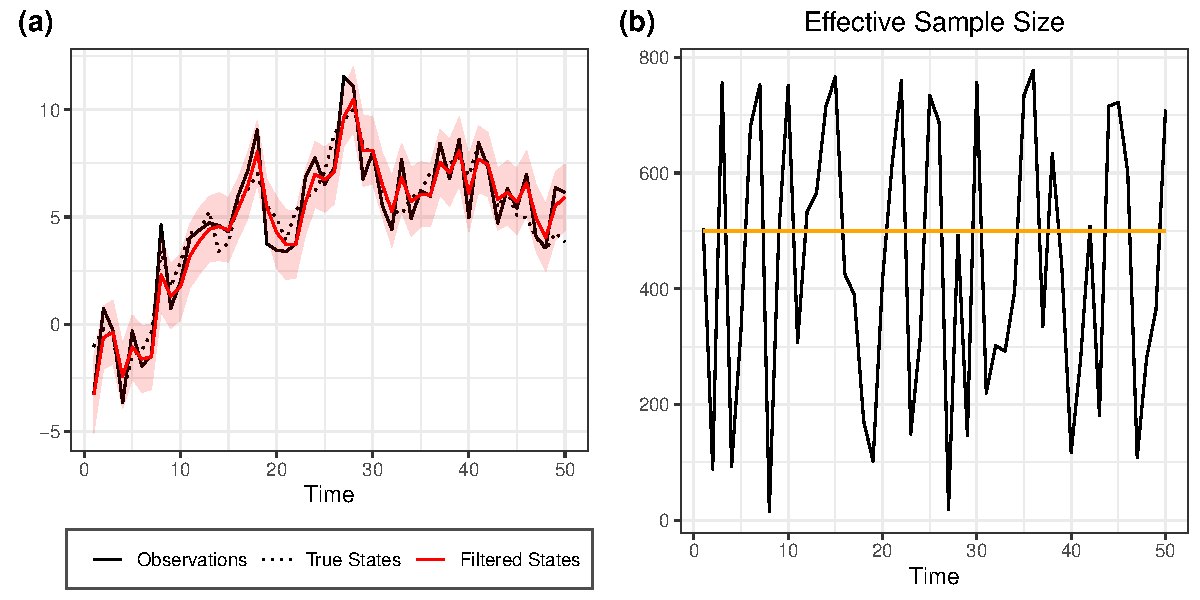
\includegraphics{prova_knit_finale_files/figure-latex/unnamed-chunk-20-1} 

}

\caption{a) APF Filtered States with credible interval (in red). b) Effective sample size (in black) with threshold (in yellow).}\label{fig:unnamed-chunk-20}
\end{figure}

Let's compare the Auxiliary Particle Filter (APF) and the Bootstrap
Particle Filter (BPF). From Figure \ref{fig:myfig6} it is difficult to
say which of the two is better and the tables does not help much since
the APF apparently outperforms the BPF in two cases over three. For this
reason we can conclude that for this model the Auxiliary Particle
Filtering strategy does not provide any serious improvement to a the
basic one.

\begin{figure}[H]

{\centering 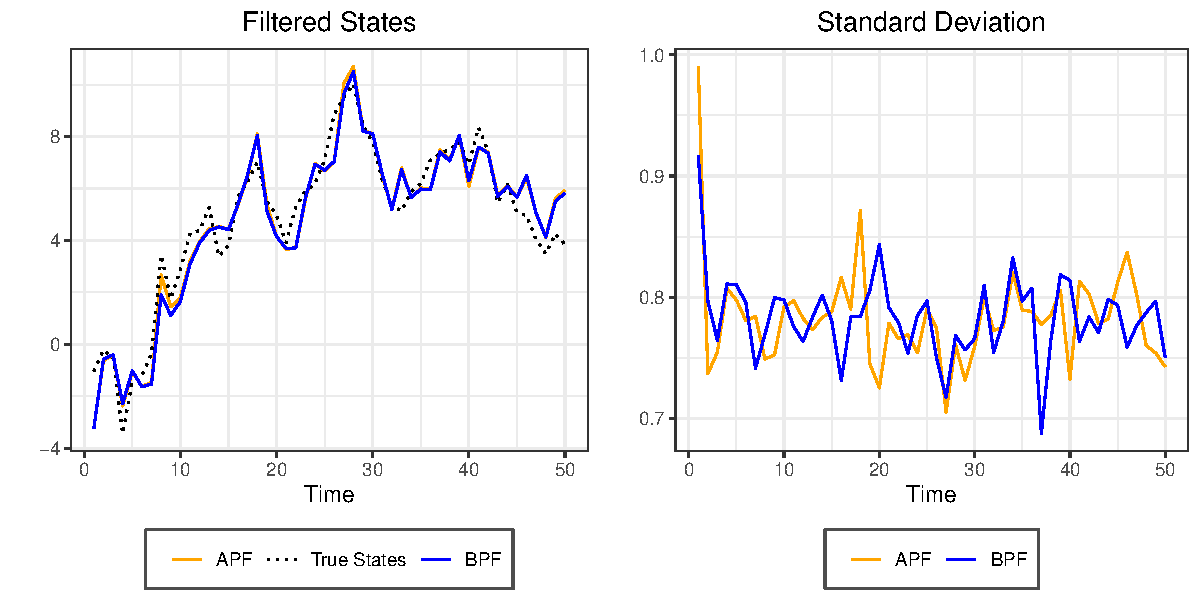
\includegraphics{prova_knit_finale_files/figure-latex/myfig6-1} 

}

\caption{Comparison Bootstrap Particle Filter(BPF) and Guided Particle Filter (GPF), number of generated particles N=1000}\label{fig:myfig6}
\end{figure}

\begin{longtable}[t]{cccc}
\caption{\label{tab:unnamed-chunk-22}Root Mean Square Errors}\\
\toprule
N & Threshold & BPF & APF\\
\midrule
1000 & 0.50 & 0.882 & 0.899\\
1000 & 0.25 & 0.889 & 0.883\\
1000 & 0.10 & 0.885 & 0.877\\
\bottomrule
\end{longtable}

We also implement the auxiliary particle filter with optimal transition
kernel. Therfore the algorithm is similiar to the one discussed above
with the difference that:

\begin{algorithm}APF with optimal transition kernel for Random Walk plus Noise Model
\begin{itemize}
\item Let $\{(x_{0},w_{0})^{(i)}\}_{i=1}^{N}$ summarizes $p(x_{0}|y_{0})$ such that, for example, $E(g(x_{0})|y_{0}) \approx \sum_{i=1}^{N}w_{0}^{(i)}g(x_{0}^{(i)})$. In particular, initialize $(x_{0}^{(1)},...,x_{0}^{(N)})$ from $N(m_{0},C_{0})$ and set $w_{0}^{(i)}=N^{-1} \ \forall \ i=1,...,N$.
\item Compute $\sigma_{opt}^{2}$ 
\item For $t=1,...,n$:
\begin{enumerate}
\item Compute $ESS=\Bigg(\sum_{i=1}^{N}(w_{t}^{(i)})^{2}\Bigg)^{-1}$
\item if $ESS<N/2$ then
\begin{enumerate}
\item Draw $I_{k}$ with $P(I_{k}=i) \propto w_{t-1}^{(i)}f_{N}(y_{t}|g(x_{t-1}^{(i)}),\sigma^{2}+\tau^{2}) $
\item Compute $\mu_{opt}=\mu(x_{t-1}^{(I_{k})})$
\item Draw $x_{t}^{(k)} \sim N(\mu_{opt},\sigma^{2}_{opt})$
\item Set  $\tilde{w}^{(i)}_{t} = N^{-1}$ for $i=1,...,N$
\end{enumerate}
\item otherwise
\begin{enumerate}
\item Compute $\mu_{opt}=\mu(x_{t-1})$
\item Draw $x_{t}^{(i)} \sim N(\mu_{opt},\sigma^{2}_{opt})$ for $i=1,...N$
\item Set $\tilde{w}^{(i)}_{t}=w^{(i)}_{t-1}f_{N}(y_{t};x_{t}^{(i)},\sigma^{2}+\tau^{2})$ for $i=1,...,N$
\end{enumerate}
\item Normalize the weights: $w_{t}^{(i)}=\frac{\tilde{w}_{t}^{(i)}}{\sum_{j=1}^{N}(\tilde{w}_{t}^{(j)})}$
\end{enumerate}
\end{itemize}
\end{algorithm}

\begin{Shaded}
\begin{Highlighting}[]
\NormalTok{APFoptfun<-}\ControlFlowTok{function}\NormalTok{(data,N,m0,C0,tau,sigma,r)\{}
  \ControlFlowTok{if}\NormalTok{(}\KeywordTok{missing}\NormalTok{(r))\{r=}\DecValTok{2}\NormalTok{\}}\ControlFlowTok{else}\NormalTok{\{\}}
\NormalTok{  xs<-}\OtherTok{NULL}
\NormalTok{  ws<-}\OtherTok{NULL}
\NormalTok{  ess<-}\OtherTok{NULL}
\NormalTok{  x  =}\StringTok{ }\KeywordTok{rnorm}\NormalTok{(N,m0,}\KeywordTok{sqrt}\NormalTok{(C0))}
\NormalTok{  importancesd<-}\KeywordTok{sqrt}\NormalTok{(tau }\OperatorTok{-}\StringTok{ }\NormalTok{tau}\OperatorTok{^}\DecValTok{2} \OperatorTok{/}\NormalTok{(tau }\OperatorTok{+}\StringTok{ }\NormalTok{sigma))}
\NormalTok{  predsd <-}\StringTok{ }\KeywordTok{sqrt}\NormalTok{(sigma}\OperatorTok{+}\NormalTok{tau)}
\NormalTok{  w  =}\StringTok{ }\KeywordTok{rep}\NormalTok{(}\DecValTok{1}\OperatorTok{/}\NormalTok{N,N)}
  
  \ControlFlowTok{for}\NormalTok{(t }\ControlFlowTok{in} \DecValTok{1}\OperatorTok{:}\KeywordTok{length}\NormalTok{(data))\{}
\NormalTok{    ESS  =}\StringTok{ }\DecValTok{1}\OperatorTok{/}\KeywordTok{sum}\NormalTok{(w}\OperatorTok{^}\DecValTok{2}\NormalTok{)}
    
    \ControlFlowTok{if}\NormalTok{(ESS}\OperatorTok{<}\NormalTok{(N}\OperatorTok{/}\NormalTok{r))\{}
\NormalTok{    weight =}\StringTok{ }\NormalTok{w}\OperatorTok{*}\KeywordTok{dnorm}\NormalTok{(data[t],x,predsd)}
\NormalTok{    k   =}\StringTok{ }\KeywordTok{sample}\NormalTok{(}\DecValTok{1}\OperatorTok{:}\NormalTok{N,}\DataTypeTok{size=}\NormalTok{N,}\DataTypeTok{replace=}\OtherTok{TRUE}\NormalTok{,}\DataTypeTok{prob=}\NormalTok{weight)}
\NormalTok{    means<-x[k]}\OperatorTok{+}\NormalTok{(tau}\OperatorTok{/}\NormalTok{(tau}\OperatorTok{+}\NormalTok{sigma))}\OperatorTok{*}\NormalTok{(data[t]}\OperatorTok{-}\NormalTok{x[k])}
\NormalTok{    x1   =}\StringTok{ }\KeywordTok{rnorm}\NormalTok{(N,means,importancesd)}
\NormalTok{    w   =}\StringTok{ }\KeywordTok{rep}\NormalTok{(}\DecValTok{1}\OperatorTok{/}\NormalTok{N,N)}
\NormalTok{    \}}\ControlFlowTok{else}\NormalTok{\{}
\NormalTok{    weight =}\StringTok{ }\KeywordTok{rep}\NormalTok{(}\DecValTok{1}\OperatorTok{/}\NormalTok{N,N)}
\NormalTok{    k   =}\StringTok{ }\KeywordTok{sample}\NormalTok{(}\DecValTok{1}\OperatorTok{:}\NormalTok{N,}\DataTypeTok{size=}\NormalTok{N,}\DataTypeTok{replace=}\OtherTok{FALSE}\NormalTok{,}\DataTypeTok{prob=}\NormalTok{weight)}
\NormalTok{    means<-x[k]}\OperatorTok{+}\NormalTok{(tau}\OperatorTok{/}\NormalTok{(tau}\OperatorTok{+}\NormalTok{sigma))}\OperatorTok{*}\NormalTok{(data[t]}\OperatorTok{-}\NormalTok{x[k])}
\NormalTok{    x1   =}\StringTok{ }\KeywordTok{rnorm}\NormalTok{(N,means,importancesd)}
\NormalTok{    w   <-}\StringTok{  }\NormalTok{w}\OperatorTok{*}\KeywordTok{dnorm}\NormalTok{(data[t],x1,predsd)}
\NormalTok{    \}}
    
\NormalTok{    w   =}\StringTok{ }\NormalTok{w}\OperatorTok{/}\KeywordTok{sum}\NormalTok{(w)}
\NormalTok{    x <-}\StringTok{ }\NormalTok{x1}
   
    
\NormalTok{    xs =}\StringTok{ }\KeywordTok{rbind}\NormalTok{(xs,x)}
\NormalTok{    ws =}\StringTok{ }\KeywordTok{rbind}\NormalTok{(ws,w)}
\NormalTok{    ess =}\KeywordTok{rbind}\NormalTok{(ess,ESS)}
    
\NormalTok{  \}}
  \KeywordTok{return}\NormalTok{(}\KeywordTok{list}\NormalTok{(}\DataTypeTok{xs=}\NormalTok{xs,}\DataTypeTok{ws=}\NormalTok{ws,}\DataTypeTok{ess=}\NormalTok{ess))}
\NormalTok{\}}
\end{Highlighting}
\end{Shaded}

\begin{figure}[H]

{\centering 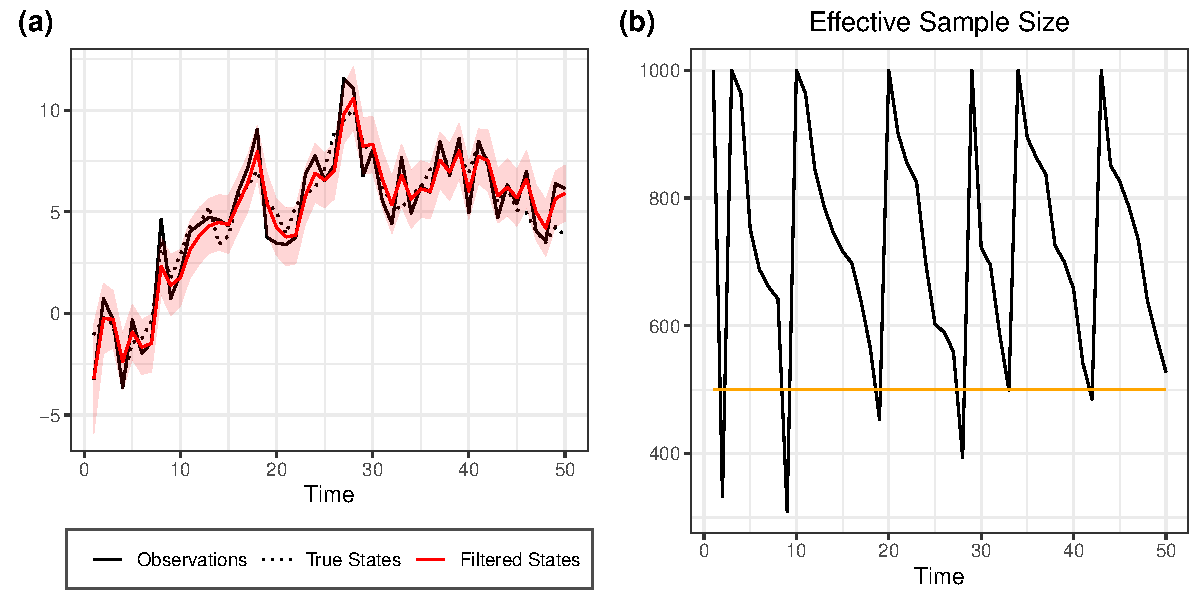
\includegraphics{prova_knit_finale_files/figure-latex/unnamed-chunk-25-1} 

}

\caption{a) APF Filtered States with credible interval (in red). b) Effective sample size (in black) with threshold (in yellow).}\label{fig:unnamed-chunk-25}
\end{figure}

\section{Liu and West Filter}\label{pf_liu_west}

Let us consider a more general state-space model, where the state vector
includes a time-constant parameter vector \(\psi \in \Psi\), where
\(\Psi\) is the parameter space. Since we can interpret the parameter as
a state with the law of motion \(\psi_t=\psi_{t-1}=\psi\), then it is
possible to adopt a PF algorithm to estimate \(\psi\).\\
However, being \(\psi\) constant over time, it is meaningless to sample
its values sequentially: the first extraction of \(\psi\) at the initial
stage 0 (i.e., \(\psi_0^n\)) generates a constant path of particles for
the parameter (\(\psi_t^n=\psi_0^n\)).
\footnote{To be more precise, at the resampling step, also $\psi^n$ is resampled, but the possible values that it may take are the $N$ ones obtained at the initial time 0 extraction.}\\
Therefore, Liu and West (2001) proposed a modified particle filter,
called \textit{Liu and West filter} (LWF) that allows to resample the
parameter over time from a continuous distribution. In this way, at
every time, the support of \(\psi\) is not limited to the \(N\)
initially sampled values.\\
Here, we describe the LWF that makes use of the normal distribution to
sample sequentially the parameter. Moreover, consider the simpler
version of the bootstrap
filter.\footnote{Clearly, the LWF can be also used within the more general frameweorks of the GPF and the APF. For instance, in our following implementation with the random walk model we use an auxiliary particle LWF.}\\
Let the transition kernel and the likelihood depend on the parameter
\(\psi\) (i.e., \(P_t(x_{t-1},dx_t;\psi)\) and \(f_t(y_t|x_t;\psi)\))
and let \(\pi(\cdot)\) be the prior distribution for the parameter
\(\psi\).\\
The LWF can be described by the following algorithm.

\begin{enumerate}
    \item \textbf{Inital stage: }For $n=1,...,N$, at time 0 sample: $X_0^n\thicksim\mathbb P_0(dx_0)$ and $\psi_0^n\thicksim \pi(\psi_0)$.
    
    Then, set the un-normalized weights $w_0^n=1$.
    
    Hence, the normalized weights are: $W_0^n=\frac{1}{N}$.
    \item \textbf{For every $t=1,...T$:}
    \begin{enumerate}
        \item \textbf{Resample} if $ESS(W_{t-1}^{1:N})<ESS_{min}$:
\begin{enumerate}
    \item Multinomial sampling for the indexes $(A_t^n)_n$ with probabilities given by $(W_{t-1}^n)_{n}$.
    \item Update weights as: $\hat w_{t-1}^n = 1$ for $n=1,...,N$.
\end{enumerate}
\textbf{Otherwise, } 
\begin{enumerate}
    \item Set the indexes: $A_t^{n}=n$ for  $n=1,...,N$
    \item Set the weights: $\hat w_{t-1}^n = w_{t-1}$ for $n=1,...,N$.
\end{enumerate}
\item \textbf{Extracting new parameter values:}
\begin{enumerate}
    \item Compute the weighted average and the variance for the parameters, respectively: $\bar \psi = \sum_{n=1}^N \hat W_{t-1}^{A_t^n}\psi^{A_t^n}$, $\Omega = \sum_{n=1}^N \hat W_{t-1}^{A_t^n}(\psi^{A_t^n}-\bar \psi)(\psi^{A_t^n}-\bar \psi)'$.\footnote{Big hat-weights $ \hat W_{t-1}^{A_t^{n}}$ are the normalized weights after the resampling stage, equal to $1/N$ if resampling takes place, $W_{t-1}^n$ otherwise.}
    \item Compute: $m^{A_t^{n}}=a \cdot  \psi^{{A_t}^{n}}+(1-a)\cdot \bar \psi$ for $n=1,...,N$, with $a\in (0,1)$ and $h^2=1-a^2$.
    \item Draw new parameters: $\psi^n\thicksim \mathcal N\big(m^{A_t^n},h^2\cdot \Omega\big)$ for $n=1,...,N$.
\end{enumerate}
\item Sample future states from the transition kernel: $X_t^n\thicksim P_t(X_{t-1}^{A_t^n},dx_t; \psi^n)$ for $n=1,...,N$.
\item Update the un-normalized weights through the likelihood function, for $n=1,...,N$:
\begin{equation*}
    w_t^n=\hat w_{t-1}^n\cdot f_t(y_t|X_t^n;\psi^n).
\end{equation*}
\item Normalize the weights, for $n=1,...,N$:  $W_t^n:=\frac{w_t^n}{\sum_{m=1}^Nw_t^m}$.
    \end{enumerate}
\end{enumerate}

At the initial step, \(N\) states and \(N\) parameter values are sampled
independently, respectively, from \(\mathbb P_0\) and \(\pi\) and the
particle weights are set to be constant, as usual.\\
Then, at each iteration (time \(t\)), the decision to resample is done
according to the \(ESS\) criterion and indexes are extracted from a
multinomial distribution. However, in the LWF both previous periods
states and parameters are resampled.\\
Meanwhile, to extract the next period states and parameters it is
necessary, firstly, to sample the new \(N\) parameter values. Let
\(\bar \psi\) be the weighted average of the parameter values and
\(\Omega\) be their variance (using the normalized weights in \(t-1\)
after the resampling step).~\\
The algorithm suggests to sample new values for the parameters from a
continuous distribution, i.e., a
Normal\footnote{More generally, distributions whose support coincides with the relevant parameter space.}
centered at the (resampled) values \(m^{A_t^n}\) with variance
\(h^2\cdot \Omega\) where \(m^n\) is a convex combination of the sample
mean \(\bar\psi\) and the actual extraction of \(\psi^n\) with
coefficient \(a\in (0,1)\) and \(h\) is a scalar such that
\(a^2+h^2=1\). While it would be more intuitively immediate to sample
new parameters from a Normal density centered at the previously sampled
values (i.e., \(\psi^n\)), this would increase the variance of \(\psi\)
over time.\\
In fact, let
\(\pi_{t-1}^N(\psi)=\sum_{n=1}^N \hat W_{t-1}^{A_t^{n}}\cdot \mathcal N(\psi^{A_t^{n}},\Omega)\)
be the empirical distribution of the parameters. From the law of
iterated expectation and total variance, we
obtain:\footnote{For completeness, we specify that the first expected value in the law of iterated expectations and total variances is with respect to the distribution of the indexes and the second one with respect to each of the Normal distributions centered at $\psi^{A_t^{n}}$.}
\begin{equation*}
    \begin{split}
        \mathbb E_{\pi_{t-1}^N} ( \psi)=& \mathbb E\big[\mathbb E( \psi|A_t^{n})\big]=\mathbb E\big[\psi^{A_t^{n}}\big]=\bar \psi\\
        Var_{\pi_{t-1}^N} ( \psi)=&Var\big[\mathbb E( \psi|A_t^{n})\big]+\mathbb E\big[Var( \psi|A_t^{n})\big]=Var\big[\psi^{A_t^{n}}\big]+\mathbb E\big[\Omega\big]=2\cdot\Omega
    \end{split}
\end{equation*} Hence, while the mean is preserved, the variance
increases at each iteration. Instead, sampling from the distribution
proposed by Liu and West
\(\mathcal N\big(m^{A_t^n},h^2\cdot \Omega\big)\) preserves both the
mean and the variance of the parameters over time.\\
Let
\(\tilde \pi_{t-1}^N(\psi)=\sum_{n=1}^N \hat W_{t-1}^{A_t^{n}}\cdot \mathcal N\big(m^{A_t^n},h^2\cdot \Omega\big)\).
Hence: \begin{equation*}
    \begin{split}
        \mathbb E_{\tilde \pi_{t-1}^N} ( \psi)=& \mathbb E\big[\mathbb E( \psi|A_t^{n})\big]=\mathbb E\big[m^{A_t^n}\big]=\mathbb E\big[a\cdot \psi^{A_t^n}+(1-a)\cdot \bar \psi\big]=\bar \psi\\
        Var_{\tilde \pi_{t-1}^N} ( \psi)=&Var\big[\mathbb E( \psi|A_t^{n})\big]+\mathbb E\big[Var( \psi|A_t^{n})\big]=Var\big[m^{A_t^n}\big]+h^2\cdot\mathbb E\big[\Omega\big]=(\underbrace{a^2+h^2}_{=1})\cdot \Omega =\Omega
    \end{split}
\end{equation*} Finally, after sampling the new \(N\) parameter values,
conditional on these values, new states are also sampled from the
transition kernel: \(X_t^n\thicksim P_t(X_{t-1}^{A_t^n},dx_t; \psi^n)\).
Lastly, weights are updated through the incremental weights.~\\
To conclude, it is worth noting that the LWF produces, together with the
usual filtering and prediction distributions, a posterior distribution
for the parameter: \begin{equation}
    \pi^N_{t}(\psi)=\pi^N(\psi|y_{1:t})=\sum_{n=1}^NW_{t}^n\delta_{\psi^n}(\psi)
\end{equation}

\subsection{Implementation}

Consider the linear Gaussian example of section \ref{implementation},
but this time with unknown variances \(\tau^{2}\) and \(\sigma^{2}\).
Thus, let \(\psi=(\sigma^{2},\tau^{2})\) be the unknown parameter vector
and assign a gamma prior for its components, \begin{align*}
\sigma^{2}  & \sim G(\alpha_{v},\beta_{v}) \\
\tau^{2}  & \sim G(\alpha_{w},\beta_{w})
\end{align*} Alternatively, assign them a uniform prior if we have no
knowledge of the hyperparameters. Note that in this model we sample from
a Gamma distribution (instead of the Normal one, as in the previous
description of the LWF) since the parameters of interest are variances,
that can take only positive values. Next, we descrive the algorithm.

\begin{algorithm} LWF for Random Walk plus Noise Model
\begin{itemize}
\item Initialize $(x_{0}^{(1)},...,x_{0}^{(N)})$ from $N(m_{0},C_{0})$, $({\sigma^{2}}^{(1)},...,{\sigma^{2}}^{(N)})$ from $G(\alpha_{v},\beta_{v})$ and $({\tau^{2}}^{(1)},...,{\tau^{2}}^{(N)})$ from $G(\alpha_{w},\beta_{w})$. Set $w_{0}^{(i)}=N^{-1} \ \forall \ i=1,...,N$. Therefore $\psi^{(i)}=({\sigma^{2}}^{(i)},{\tau^{2}}^{(i)})$, and
$\hat{\pi}_{0}=p(x_{0}|y_{0})=\sum_{i=1}^{N}w_{0}^{(i)}\delta_{(x_{0}^{(i)},\psi^{(i)})}$
\item For $t=1,...,n$:.
\begin{enumerate}
\item Compute
\begin{align*}
\overline{\sigma^{2}}& =E_{\hat{\pi}_{t-1}}(\sigma^{2})\\
\overline{\tau^{2}}& =E_{\hat{\pi}_{t-1}}(\tau^{2}) \\
\Sigma_{v} & =V_{\hat{\pi}_{t-1}}(\sigma^{2}) \\
\Sigma_{w} & =V_{\hat{\pi}_{t-1}}(\tau^{2})
\end{align*}
then set
\begin{align*}
m_{v}^{(i)} & = a{\sigma^{2}}^{(i)}+(1-a)\overline{\sigma^{2}} \\
{s_{v}^{2}}^{(i)} & =(1-a^{2})\Sigma_{\sigma^{2}} \\
\alpha_{v}^{(i)} & =\frac{(m_{v}^{(i)})^{2}}{{s_{v}^{2}}^{(i)}} \\
\beta_{v}^{(i)} & =\frac{(m_{v}^{(i)})}{{s_{v}^{2}}^{(i)}}\\
m_{w}^{(i)} & = a{\tau^{2}}^{(i)}+(1-a)\overline{\tau^{2}} \\
{s_{w}^{2}}^{(i)} & =(1-a^{2})\Sigma_{\tau^{2}}\\
\alpha_{w}^{(i)} & =\frac{(m_{w}^{(i)})^{2}}{{s_{w}^{2}}^{(i)}} \\
\beta_{w}^{(i)} & =\frac{(m_{w}^{(i)})}{{s_{w}^{2}}^{(i)}}
\end{align*}
\item For $k=1,...,N$:
\begin{itemize}
\item Draw $I_{k}$, with $P(I_{k}=i) \propto w_{t-1}^{(i)}f_{N}(y_{t}|g(x_{t-1}^{(i)}),m_{v}) $
\item Draw ${\sigma^{2}}^{(k)}$ from $G(\alpha_{v}^{(I_k)},\beta_{v}^{(I_k)})$ 
\item Draw ${\tau^{2}}^{(k)}$ from $G(\alpha_{w}^{(I_k)},\beta_{w}^{(I_k)})$
\item Draw $x_{t}^{(k)}$ from $N(x_{t-1}^{(I_k)},{\tau^2}^{(k)})$
\item Set  $\tilde{w}_{t}^{(k)} = \frac{f_{N}(y_{t}|x_{t}^{(k)},{\sigma^2}^{(k)})}{f_{N}(y_{t}|g(x_{t-1}^{(I_{k})},m_{v}^{(I_k)}))}$
\end{itemize}
\item Compute $ESS=\Bigg(\sum_{i=1}^{N}(w_{t}^{(i)})^{2}\Bigg)^{-1}$
\item if $ESS<N/2$ then
\begin{enumerate}
\item Draw a sample of size N, $(x_{t}^{(1)},...,x_{t}^{(N)})$, from the discrete distribution $P(x_{t}=x_{t}^{(i)})=w_{t}^{(i)},\ \ i=1,...,N$
\item Reset the weights: $w_{t}^{(i)}=N^{-1}$, $i=1,...,N$.
\end{enumerate}
\item Set $\hat{\pi}_{t}=p(x_{t}|y_{1:t})=\sum_{i=1}^{N}w_{t}^{(i)}\delta_{(x_{t}^{(i)},\psi^{(i)})}$
\end{enumerate}
\end{itemize}
\end{algorithm}

Our \texttt{LWfun} function goes through the illustrated steps.\\

\hrule
\hrule

\texttt{LWfun(data,N,m0,C0,alphav,betav,alphaw,betaw,delta,unif,r)}\\

\hrule

\textbf{Arguments}

\texttt{data} ~~the observed process. It has to be a vector or a
univariate time series.\\
\texttt{N} ~~number of particles generated at each step\\
\texttt{m0} ~~central value of the normal prior state distribution\\
\texttt{C0} ~~variance of the normal prior state distribution\\
\texttt{alphav, betav} ~~ Gamma prior hyperparameters on
\(\sigma^{2}\)\\
\texttt{alphaw,betaw} ~~ Gamma prior hyperparameters on \(\tau^{2}\)\\
\texttt{delta} ~~hyperparameter delta value\\
\texttt{unif} ~~if True then it sets a Uniform \((0,10)\) prior on
\(\sigma^{2}\) and \(\tau^{2}\)\\
\texttt{r} ~~ if present the threshold is set equal to \(N/r\)
otherwise, if missing, the threshold is set equal to \(N/2\)

\hrule
\hrule

\begin{Shaded}
\begin{Highlighting}[]
\NormalTok{LWfun<-}\ControlFlowTok{function}\NormalTok{(data,N,m0,C0,alphav,betav,alphaw,betaw,delta,unif,r)\{}
  \ControlFlowTok{if}\NormalTok{(}\KeywordTok{missing}\NormalTok{(r))\{r=}\DecValTok{2}\NormalTok{\}}\ControlFlowTok{else}\NormalTok{\{\}}
\NormalTok{  xs     =}\StringTok{ }\KeywordTok{rnorm}\NormalTok{(N,m0,}\KeywordTok{sqrt}\NormalTok{(C0))}
  \ControlFlowTok{if}\NormalTok{(unif}\OperatorTok{==}\NormalTok{T)\{}
\NormalTok{  pars   =}\StringTok{ }\KeywordTok{cbind}\NormalTok{(}\KeywordTok{runif}\NormalTok{(N,}\DecValTok{0}\NormalTok{,}\DecValTok{10}\NormalTok{),}\KeywordTok{runif}\NormalTok{(N,}\DecValTok{0}\NormalTok{,}\DecValTok{10}\NormalTok{))\}}\ControlFlowTok{else}\NormalTok{\{\}}
\NormalTok{  pars   =}\StringTok{ }\KeywordTok{cbind}\NormalTok{(}\KeywordTok{rgamma}\NormalTok{(N,}\DataTypeTok{shape=}\NormalTok{alphav,}\DataTypeTok{scale=}\NormalTok{betav),}\KeywordTok{rgamma}\NormalTok{(N,}\DataTypeTok{shape=}\NormalTok{alphaw,}\DataTypeTok{scale=}\NormalTok{betaw))}
\NormalTok{  a      =}\StringTok{ }\NormalTok{(}\DecValTok{3}\OperatorTok{*}\NormalTok{delta}\DecValTok{-1}\NormalTok{)}\OperatorTok{/}\NormalTok{(}\DecValTok{2}\OperatorTok{*}\NormalTok{delta)}
\NormalTok{  h2     =}\StringTok{ }\DecValTok{1}\OperatorTok{-}\NormalTok{a}\OperatorTok{^}\DecValTok{2}
\NormalTok{  parss  =}\StringTok{ }\KeywordTok{array}\NormalTok{(}\DecValTok{0}\NormalTok{,}\KeywordTok{c}\NormalTok{(N,}\DecValTok{2}\NormalTok{,n))}
\NormalTok{  xss    =}\StringTok{ }\OtherTok{NULL}
\NormalTok{  ws     =}\StringTok{ }\OtherTok{NULL}
\NormalTok{  ess    =}\StringTok{ }\OtherTok{NULL}
\NormalTok{  w      =}\StringTok{ }\KeywordTok{rep}\NormalTok{(}\DecValTok{1}\OperatorTok{/}\NormalTok{N,N)}
  \ControlFlowTok{for}\NormalTok{ (t }\ControlFlowTok{in} \DecValTok{1}\OperatorTok{:}\KeywordTok{length}\NormalTok{(data))\{}
\NormalTok{    meanV =}\StringTok{ }\KeywordTok{weighted.mean}\NormalTok{(pars[,}\DecValTok{1}\NormalTok{],w)}
\NormalTok{    varV  =}\StringTok{ }\KeywordTok{weighted.mean}\NormalTok{((pars[,}\DecValTok{1}\NormalTok{]}\OperatorTok{-}\NormalTok{meanV)}\OperatorTok{^}\DecValTok{2}\NormalTok{,w)}
\NormalTok{    meanW =}\StringTok{ }\KeywordTok{weighted.mean}\NormalTok{(pars[,}\DecValTok{2}\NormalTok{],w)}
\NormalTok{    varW  =}\StringTok{ }\KeywordTok{weighted.mean}\NormalTok{((pars[,}\DecValTok{2}\NormalTok{]}\OperatorTok{-}\NormalTok{meanW)}\OperatorTok{^}\DecValTok{2}\NormalTok{,w)}
    
\NormalTok{    muV =}\StringTok{ }\NormalTok{a}\OperatorTok{*}\NormalTok{pars[,}\DecValTok{1}\NormalTok{]}\OperatorTok{+}\NormalTok{(}\DecValTok{1}\OperatorTok{-}\NormalTok{a)}\OperatorTok{*}\NormalTok{meanV}
\NormalTok{    sigma2V =}\StringTok{ }\NormalTok{(}\DecValTok{1}\OperatorTok{-}\NormalTok{a}\OperatorTok{^}\DecValTok{2}\NormalTok{)}\OperatorTok{*}\NormalTok{varV}
\NormalTok{    alphaV =}\StringTok{ }\NormalTok{muV}\OperatorTok{^}\DecValTok{2}\OperatorTok{/}\NormalTok{sigma2V}
\NormalTok{    betaV =}\StringTok{ }\NormalTok{muV}\OperatorTok{/}\NormalTok{sigma2V}
    
\NormalTok{    muW =}\StringTok{ }\NormalTok{a}\OperatorTok{*}\NormalTok{pars[,}\DecValTok{2}\NormalTok{]}\OperatorTok{+}\NormalTok{(}\DecValTok{1}\OperatorTok{-}\NormalTok{a)}\OperatorTok{*}\NormalTok{meanW}
\NormalTok{    sigma2W =}\StringTok{ }\NormalTok{(}\DecValTok{1}\OperatorTok{-}\NormalTok{a}\OperatorTok{^}\DecValTok{2}\NormalTok{)}\OperatorTok{*}\NormalTok{varW}
\NormalTok{    alphaW =}\StringTok{ }\NormalTok{muW}\OperatorTok{^}\DecValTok{2}\OperatorTok{/}\NormalTok{sigma2W}
\NormalTok{    betaW =}\StringTok{ }\NormalTok{muW}\OperatorTok{/}\NormalTok{sigma2W}
    
\NormalTok{    weight      =}\StringTok{ }\NormalTok{w}\OperatorTok{*}\KeywordTok{dnorm}\NormalTok{(data[t],xs,}\KeywordTok{sqrt}\NormalTok{(muV))}
\NormalTok{    k           =}\StringTok{ }\KeywordTok{sample}\NormalTok{(}\DecValTok{1}\OperatorTok{:}\NormalTok{N,}\DataTypeTok{size=}\NormalTok{N,}\DataTypeTok{replace=}\NormalTok{T,}\DataTypeTok{prob=}\NormalTok{weight)}
    
\NormalTok{    pars[,}\DecValTok{1}\NormalTok{]<-}\KeywordTok{rgamma}\NormalTok{(N,}\DataTypeTok{shape=}\NormalTok{alphaV[k],}\DataTypeTok{rate=}\NormalTok{betaV[k])}
\NormalTok{    pars[,}\DecValTok{2}\NormalTok{]<-}\KeywordTok{rgamma}\NormalTok{(N,}\DataTypeTok{shape=}\NormalTok{alphaW[k],}\DataTypeTok{rate=}\NormalTok{betaW[k])}
    
\NormalTok{    xsprevious<-xs[k]}
\NormalTok{    xs =}\StringTok{ }\KeywordTok{rnorm}\NormalTok{(N,xs[k],}\KeywordTok{sqrt}\NormalTok{(pars[,}\DecValTok{2}\NormalTok{]))}
    
\NormalTok{    w           =}\StringTok{ }\KeywordTok{exp}\NormalTok{(}\KeywordTok{dnorm}\NormalTok{( data[t],xs,}\KeywordTok{sqrt}\NormalTok{(pars[,}\DecValTok{1}\NormalTok{]),}\DataTypeTok{log=}\NormalTok{T)}\OperatorTok{-}
\StringTok{                        }\KeywordTok{dnorm}\NormalTok{( data[t],xsprevious,}\KeywordTok{sqrt}\NormalTok{(muV[k]),}\DataTypeTok{log=}\NormalTok{T))}
\NormalTok{    w           =}\StringTok{ }\NormalTok{w}\OperatorTok{/}\KeywordTok{sum}\NormalTok{(w)}
\NormalTok{    ESS         =}\StringTok{ }\DecValTok{1}\OperatorTok{/}\KeywordTok{sum}\NormalTok{(w}\OperatorTok{^}\DecValTok{2}\NormalTok{)}
    
    \ControlFlowTok{if}\NormalTok{(ESS}\OperatorTok{<}\NormalTok{(N}\OperatorTok{/}\NormalTok{r))\{}
\NormalTok{      index<-}\KeywordTok{sample}\NormalTok{(N,}\DataTypeTok{size=}\NormalTok{N,}\DataTypeTok{replace=}\NormalTok{T,}\DataTypeTok{prob=}\NormalTok{w)}
\NormalTok{      xs<-xs[index]}
\NormalTok{      pars<-pars[index,]}
\NormalTok{      w<-}\KeywordTok{rep}\NormalTok{(}\DecValTok{1}\OperatorTok{/}\NormalTok{N,N)}
\NormalTok{    \}}\ControlFlowTok{else}\NormalTok{\{}
\NormalTok{      xs<-xs}
\NormalTok{      pars<-pars}
\NormalTok{    \}}
    
    
\NormalTok{    xss         =}\StringTok{ }\KeywordTok{rbind}\NormalTok{(xss,xs)}
\NormalTok{    parss[,,t]  =}\StringTok{ }\NormalTok{pars }
\NormalTok{    ws          =}\StringTok{ }\KeywordTok{rbind}\NormalTok{(ws,w)}
\NormalTok{    ess         =}\StringTok{ }\KeywordTok{rbind}\NormalTok{(ess,ESS)}
\NormalTok{  \}}
  \KeywordTok{return}\NormalTok{(}\KeywordTok{list}\NormalTok{(}\DataTypeTok{xss=}\NormalTok{xss,}\DataTypeTok{parss=}\NormalTok{parss,}\DataTypeTok{ws=}\NormalTok{ws,}\DataTypeTok{ess=}\NormalTok{ess))}
\NormalTok{\}}
\end{Highlighting}
\end{Shaded}

We provide an example of Liu and West filter fixing \(\delta=0.7\) and
drawing \(\alpha_{v}\), \(\beta_{v}\), \(\alpha_{w}\) and \(\beta_{w}\)
from a Uniform \(U(0,10)\). The results are shown in the following
figure.

\begin{figure}[H]

{\centering 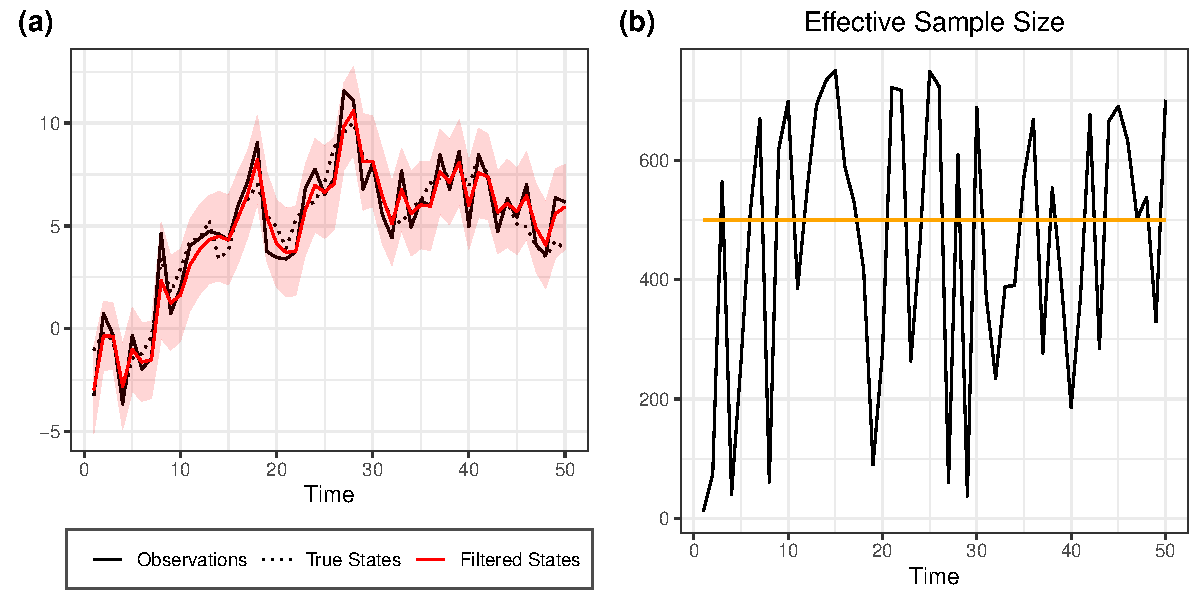
\includegraphics{prova_knit_finale_files/figure-latex/unnamed-chunk-28-1} 

}

\caption{a) LW Filtered States with credible interval (in red). b) Effective sample size (in black) with threshold (in yellow).}\label{fig:unnamed-chunk-28}
\end{figure}

Finally, we compare the performances of the Liu and West filter and the
other filtering strategies discussed so far. As we expect, in the linear
Gaussian case, Kalman filter outperforms the other strategies. On the
other hand, the Liu and West, with hyperparameters setted as described
above, provides the worst estimates in terms of RMSE. This is not
necessarily due to an overall weakness of the LWF with respect to the
other filters, but simply to a not accurate choice of the
hyperparameters. Moreover, while increasing the number of particles
improves the accuracy, notice that the threshold for ESS-based
resampling is not strictly related to better performances.

\begin{longtable}[t]{cccccc}
\caption{\label{tab:unnamed-chunk-30}RMSE}\\
\toprule
N & Threshold & KF & BPF & APF & LWF\\
\midrule
100 & 0.50 & 0.879 & 0.916 & 0.881 & 0.883\\
1000 & 0.50 & 0.879 & 0.882 & 0.899 & 0.977\\
10000 & 0.50 & 0.879 & 0.885 & 0.874 & 0.945\\
1000 & 0.50 & 0.879 & 1.172 & 1.677 & 1.140\\
1000 & 0.25 & 0.879 & 1.085 & 0.974 & 3.419\\
\addlinespace
1000 & 0.10 & 0.879 & 4.285 & 0.994 & 1.142\\
\bottomrule
\end{longtable}

\section{Convergence}\label{pf_converg}

In this section, we cover three propositions that justify the use of the
PF algorithms to estimate quantities of interest. Firstly, we present
two convergence results for the estimators of the predictive and
filtering distributions. As we will discuss, these results hold under
reasonable conditions. Then, we will show that the error of the particle
estimators are asymptotically distributed according to a Gaussian
distribution with known variance. Henceforth, we will maintain the
assumption that (multinomial) resampling is repeated at each iteration.

\subsection{MSE convergence}

As already seen in subsection \ref{seq_impt_sampling}, the particle
approximation of \(\mathbb Q_{t}(dx_{0:t})\) is: \begin{equation*}
      \sum_{n=1}^NW_{t-1}^nM_t(X_{t-1}^n,dx_t).
\end{equation*} The following lemma states that the (mean squared) error
related to sampling from this conditional distribution is bounded.
\bigskip

\begin{lemma}
For any measurable, integrable, and bounded function $\varphi:\mathcal X\rightarrow\mathbb R,$
$$
\mathbb E\Bigg[ \bigg\{ \frac{1}{N} \sum\limits_{n=1}^N \varphi(X_t^n)-\sum\limits_{n=1}^NW_{t-1}^n(M_t\varphi)(X_{t-1}^n) \bigg\}^2 \Bigg]\leq \frac{\|\varphi\|_{\infty}^2}{N},
$$
where $\|\cdot\|_{\infty}$ is the supnorm and $M_t\varphi$ is the map 
$x_{t-1}\mapsto \int_{\mathcal X}M_t(x_{t-1},dx_t)\varphi(x_t).$
\end{lemma}

This result can be used to prove the convergence of the estimator
\(\frac{1}{N} \sum\limits_{n=1}^N \varphi(X_t^n)\). To see this, note
that \begin{equation}
    \begin{split}
        \frac{1}{N} \sum\limits_{n=1}^N \varphi(X_t^n)-\mathbb E_{\mathbb Q_{t-1}M_t}(\varphi)=\bigg(&\frac{1}{N} \sum\limits_{n=1}^N \varphi(X_t^n)-\sum\limits_{n=1}^NW_{t-1}^n(M_t\varphi)(X_{t-1}^n) \bigg) \\
        & + \bigg(\sum\limits_{n=1}^NW_{t-1}^n(M_t\varphi)(X_{t-1}^n)- \mathbb E_{\mathbb Q_{t-1}M_t}(\varphi)\bigg).
    \end{split}
\end{equation} where
\(\mathbb E_{\mathbb Q_{t-1}M_t}(\varphi)=\int_{\mathcal X^{t+1}}\varphi(x_t) \mathbb Q_{t-1}(dx_{0:t-1})M_t(x_{t-1},dx_t)\).\\
By the lemma, the first component of the right-hand side has a bounded
MSE. It can be proved that also the second component of the right-hand
side has a bounded MSE. Using the fact that
\(\mathbb E\{(X+Y)^2\}\leq2\mathbb E\{\mathbb E(X^2)+\mathbb E(Y^2)\},\)
it follows that also the MSE of the left-hand side is bounded. A simple
induction argument proves that the result holds for all \(t\).\\
Using a similar argument, one can prove that the MSE of the estimator
\(\sum\limits_{n=1}^N W_t^n \varphi(X_t^n)\) is bounded as well. These
ideas are formalized in the following proposition. \bigskip

\begin{proposition}
For any measurable, integrable, and bounded function $\varphi:\mathcal X\rightarrow\mathbb R,$ $\forall t\geq0$ there exist constants $c_t,c_t'$ such that:
$$
\mathbb E\Bigg[ \bigg\{ \frac{1}{N} \sum\limits_{n=1}^N \varphi(X_t^n)-\mathbb E_{\mathbb Q_{t-1}M_t}(\varphi)\bigg\}^2 \Bigg]\leq c_t \frac{\|\varphi\|_{\infty}^2}{N}
$$
and 
$$
    \mathbb E\Bigg[ \bigg\{\sum\limits_{n=1}^N W_t^n \varphi(X_t^n)-\mathbb E_{\mathbb Q_t}(\varphi) \bigg\}^2 \Bigg]\leq c_t' \frac{\|\varphi\|_{\infty}^2}{N}.
$$
Therefore, taking the limit for $N\rightarrow \infty,$ we have that 
$$
\frac{1}{N} \sum\limits_{n=1}^N \varphi(X_t^n)\xrightarrow{\text{MSE}}\mathbb E_{\mathbb Q_{t-1}M_t}(\varphi)
$$
and 
$$
\sum\limits_{n=1}^N W_t^n \varphi(X_t^n)\xrightarrow{\text{MSE}}\mathbb E_{\mathbb Q_t}(\varphi)
$$
\end{proposition}

In the next subsection, we establish a much stronger property of the
particle filter algorithms.

\subsection{Almost sure convergence}

The following proposition states that estimators
\(\frac{1}{N} \sum\limits_{n=1}^N \varphi(X_t^n)\) and
\(\sum\limits_{n=1}^N W_t^n \varphi(X_t^n)\) converge to their true
values, up to negligible sets, i.e., the sets such that the estimators
do not converge to \(\mathbb E_{\mathbb Q_{t-1}M_t}(\varphi)\) and
\(\mathbb E_{\mathbb Q_t}(\varphi)\) have zero probability.
Additionally, recall that almost sure convergence implies convergence in
probability. \bigskip

\begin{proposition}
For any $t\geq0$ and any measurable, integrable, and bounded function $\varphi:\mathcal X\rightarrow\mathbb R,$
$$
\frac{1}{N} \sum\limits_{n=1}^N \varphi(X_t^n)\xrightarrow{\text{a.s}}\mathbb E_{\mathbb Q_{t-1}M_t}(\varphi)
$$
and 
$$
\sum\limits_{n=1}^N W_t^n \varphi(X_t^n)\xrightarrow{\text{a.s}}\mathbb E_{\mathbb Q_{t}}(\varphi).
$$
\end{proposition}

\subsection{Central limit theorem}

The last asymptotic result of PF estimators concerns convergence in law:
the error of a particle estimate is asymptotically normally distributed.
\bigskip

\begin{proposition}
For any $t\geq0$ and any measurable, integrable, and bounded function $\varphi:\mathcal X\rightarrow\mathbb R,$
$$
\sqrt{N}\bigg( \frac{1}{N} \sum\limits_{n=1}^N \varphi(X_t^n)-\mathbb E_{\mathbb Q_{t-1}M_t}(\varphi)\bigg)\implies \mathcal N(0,\hat{\mathcal{V}}_t(\varphi))
$$
and 
$$
\sqrt{N}\bigg(\sum\limits_{n=1}^N W_t^n \varphi(X_t^n)-\mathbb E_{\mathbb Q_{t}}(\varphi)\bigg)\implies \mathcal N(0,\mathcal{V}_t(\varphi)),
$$
where the asymptotic variances are defined recursively, with $ \hat{\mathcal{V}}_0(\varphi):=Var_{\mathbb M_0}(\varphi) $,
\begin{equation*}
    \begin{split}
        \hat{\mathcal{V}}_t(\varphi)&:=\mathcal{V}_{t-1}(\mathbb E_{M_t}(\varphi))+Var_{\mathbb Q_{t-1}M_t}(\varphi) \text{ }\forall t\geq1, \\
        \mathcal{V}_t(\varphi)&:=\hat{\mathcal{V}}_{t}\big( \bar{G}_t(\varphi-\mathbb E_{\mathbb Q_t}(\varphi)) \big) \text{ }\forall t\geq0.
    \end{split}
\end{equation*}
Here, $\bar{G}_t=G_t/\mathbb E_{\mathbb Q_{t-1}M_t}(G_t)$ is the normalized incremental weight.
\end{proposition}

This version of the CLT for PF suggest that PF estimators with respect
both to the predictive and the filtering distributions are approximately
normal for a large number of particles.\\
In particular, the logic behind the expression for
\(\mathcal{V}_t(\varphi)\) is the same as described in section
\ref{pf_is_conv}. In fact, recall that the estimator with respect to the
filtering distribution is a more sophisticated form of IS estimator,
where the target distribution differs from the proposal one. ~ Instead,
to get an intuition of the variance \(\hat{\mathcal{V}}_t(\varphi),\)
note that by the law of total variance, \begin{equation*}
    \begin{split}
        Var\Bigg[ \frac{1}{N}  \sum\limits_{n=1}^N \varphi(X_t^n) \Bigg] = &Var\Bigg[ \mathbb E\bigg[\frac{1}{N}  \sum\limits_{n=1}^N \varphi(X_t^n)\Big| \sigma(X_{t-1}^{1:N}) \bigg] \Bigg] \\
        &+ \mathbb E\Bigg[ Var\bigg[ \frac{1}{N}  \sum\limits_{n=1}^N \varphi(X_t^n)    \Big| \sigma(X_{t-1}^{1:N})\bigg]\Bigg] \\
        &= Var\bigg[\sum\limits_{n=1}^N W_{t-1}^n (M_t\varphi)(X_{t-1}^n)\bigg] \\
        &+\frac{1}{N}\mathbb E\Bigg[Var\bigg[\varphi(X_t^1) \Big| \sigma(X_{t-1}^{1:N})\bigg]\Bigg].
    \end{split}
\end{equation*} The notation \(\mid \sigma(X_{t-1}^{1:N})\) means
conditioning on having sampled (from the multinomial distribution)
\(X_{t-1}^{1:N}\). Conditional on multinomial sampling, the
\(X_{t-1}^n\) are i.i.d., with distribution
\(\sum\limits_{n=1}^N W_{t-1}^n M_t(X_{t-1}^n, dx_t)\), that should
converge to \(\mathbb Q_{t-1}M_t\). So, it is natural to think that the
second element of the sum converges to the variance of \(\varphi\) with
respect to the distribution \(\mathbb Q_{t-1}M_t\). These results are of
practical use because they provide a way to explicitly compute the
variance of the PF estimates.

\section{Implementations for Stochastic Volatility Models}

So far we have seen Sequential Monte Carlo methods applied to the linear
Gaussian case, however, as already mentioned, for this class of state
space models, Kalman Filter provides a closed form solution. Here, we
want to provide an illustration of Particle Filters for a state space
model for which no analytical solutions are available. More precisely,
we deal with a stochastic volatility model. For the sake of simplicity
we use a basic specification of stochastic volatility model

\begin{align}
y_{t}|x_{t} & \sim N(0,e^{x_{t}}) \\
x_{t}|x_{t-1} & \sim N(\alpha+\beta x_{t-1},\tau^2)
\end{align}

We start describing the main four particle filtering strategies
discussed in this work and then we are going to compare their
performances. The R code of these and other algorithms used in the
Chapter application can be found in Appendix 1.

In the Bootstrap Particle filter we basically use the model transition
kernel and do resampling any time the effective sample size is smaller
than a predetermined threshold.

\begin{algorithm} BPF for Stochastic Volatility Model
\begin{itemize}
\item Let $\{(x_{0},w_{0})^{(i)}\}_{i=1}^{N}$ summarize $p(x_{0}|y_{0})$ such that, for example, $E(g(x_{0})|y_{0}) \approx \sum_{i=1}^{N}w_{0}^{(i)}g(x_{0}^{(i)})$. In particular, initialize $(x_{0}^{(1)},...,x_{0}^{(N)})$ form $N(m_{0},C_{0})$ and set $w_{0}^{(i)}=N^{-1} \ \forall \ i=1,...,N$.
\item For $t=1,...,n$:
\begin{enumerate}
\item Draw $x_{t}^{(i)} \sim N(\alpha+\beta x_{t-1},\tau^2) \ \ i=1,...,N$ such that $\{(x_{t},w_{t-1})^{(i)}\}_{i=1}^{N}$ summarizes $p(x_{t}|y_{1:t-1})$
\item Set $w_{t}^{(i)} = w_{t-1}^{(i)}f_{N}(y_{t};0,e^{x_{t}}) \ \ i=1,...,N$ such that $\{(x_{t},w_{t})^{(i)}\}_{i=1}^{N}$ summarizes $p(x_{t}|y_{1:t})$
\item Normalize the weights: $w_{t}^{(i)}=\frac{\tilde{w}_{t}^{(i)}}{\sum_{j=1}^{N}(\tilde{w}_{t}^{(j)})}$
\item Compute $ESS=\Bigg(\sum_{i=1}^{N}(w_{t}^{(i)})^{2}\Bigg)^{-1}$
\item if $ESS<N/2$ then
\begin{enumerate}
\item Draw a sample of size N, $(x_{t}^{(1)},...,x_{t}^{(N)})$, from the discrete distribution $P(x_{t}=x_{t}^{(i)})=w_{t}^{(i)},\ \ i=1,...,N$
\item Reset the weights: $w_{t}^{(i)}=N^{-1}$, $i=1,...,N$.
\end{enumerate}
\item Set $p(x_{t}|y_{1:t})=\sum_{i=1}^{N}w_{t}^{(i)}\delta_{x_{t}^{(i)}}$
\end{enumerate}
\end{itemize}
\end{algorithm}

If we instead want to sample from the optimal transition kernel, things
get more complicated. It can be shown that the optimal transition kernel
is
\[ m_{t}^{opt}(x_{t}|x_{t-1}) \propto f_{t}(y_{t}|x_{t})p(x_{t}|x_{t-1}) \propto exp\bigg[-\frac{1}{2\sigma^{2}}(x_{t}-\alpha-\beta x_{t-1})^{2}-\frac{e^{-x_{t}}}{2}y_{t}^{2}-\frac{x_{t}}{2}\bigg]\]
and it is not straightforward to sample from it. Therefore, we follow a
common praxis consisting in approximating \(m_{t}^{opt}\) by a Gaussian
distribution obtained by linearising \(e^{-x_{t}}\),
i.e.~\(e^{-x_{t}}=e^{-x_{0}}(1+x_{0}-x+...)\), taking
\(x_{0}=\mu^{\star}(x_{t-1}) := \alpha + \beta x_{t-1}\), i.e the mean
of the Gaussian transition density \(p(x_{t}|x_{t-1})\). After some
calculations we would end up with a Gaussian distribution
\(N(\xi(x_{t-1}),\sigma^{2})\) with
\[ \xi(x_{t-1}) = \mu^{\star}(x_{t-1}) + \frac{\sigma^{2}}{4}(y_{t}^{2}e^{-\mu^{\star}(x_{t-1})}-2)\].
With this transition kernel we can implement the Guided Particle Filter
in the following way

\begin{algorithm} GPF for Stochastic Volatility Model
\begin{itemize}
\item Let $\{(x_{0},w_{0})^{(i)}\}_{i=1}^{N}$ summarize $p(x_{0}|y_{0})$ such that, for example, $E(g(x_{0})|y_{0}) \approx \sum_{i=1}^{N}w_{0}^{(i)}g(x_{0}^{(i)})$. In particular, initialize $(x_{0}^{(1)},...,x_{0}^{(N)})$ from $N(m_{0},C_{0})$ and set $w_{0}^{(i)}=N^{-1} \ \forall \ i=1,...,N$.
\item For $t=1,...,n$:
\begin{enumerate}
\item Draw $x_{t}^{(i)} \sim N(\alpha+\beta x_{t-1}+\frac{\tau^2}{4}\big[y_{t}^2e^{-(\alpha+\beta x_{t-1})}-2\big],\tau^{2}) \ \ i=1,...,N$ such that $\{(x_{t},w_{t-1})^{(i)}\}_{i=1}^{N}$ summarizes $p(x_{t}|y_{1:t-1})$
\item Set $w_{t}^{(i)} = w_{t-1}^{(i)}\frac{f_{N}(y_{t};0,e^{x_{t}})f_{N}(x_{t};\alpha+\beta x_{t-1},\tau^{2})}{f_{N}(x_{t};\alpha+\beta x_{t-1}+\frac{\tau^2}{4}\big[y_{t}^2e^{-(\alpha+\beta x_{t-1})}-2\big],\tau^{2})} \ \ i=1,...,N$ such that $\{(x_{t},w_{t})^{(i)}\}_{i=1}^{N}$ summarizes $p(x_{t}|y_{1:t})$
\item Normalize the weights: $w_{t}^{(i)}=\frac{\tilde{w}_{t}^{(i)}}{\sum_{j=1}^{N}(\tilde{w}_{t}^{(j)})}$
\item Compute $ESS=\Bigg(\sum_{i=1}^{N}(w_{t}^{(i)})^{2}\Bigg)^{-1}$
\item if $ESS<N/2$ then
\begin{enumerate}
\item Draw a sample of size N, $(x_{t}^{(1)},...,x_{t}^{(N)})$, from the discrete distribution $P(x_{t}=x_{t}^{(i)})=w_{t}^{(i)},\ \ i=1,...,N$
\item Reset the weights: $w_{t}^{(i)}=N^{-1}$, $i=1,...,N$.
\end{enumerate}
\item Set $p(x_{t}|y_{1:t})=\sum_{i=1}^{N}w_{t}^{(i)}\delta_{x_{t}^{(i)}}$
\end{enumerate}
\end{itemize}
\end{algorithm}

The Auxiliary Particle Filter with optimal transition kernel uses the
same transition kernel of the Guided Particle Filter and while the
perfectly adapted auxiliary function is
\[g(x_{t-1})=\frac{1}{2\pi\sigma^{2}}\int_{\mathcal{X}}exp\bigg[-\frac{1}{2\sigma^{2}}(x_{t}-\alpha-\beta x_{t-1})^{2}-\frac{e^{-x_{t}}}{2}y_{t}^{2}-\frac{x_{t}}{2}\bigg] dx_{t-1}\]
The relevant literature suggest to approximate this integral by
linearising the exponential term as in the GPF case. The resulting
auxiliary function is
\[ g(x_{t-1})=exp \bigg[ \frac{1}{2\sigma^{2}} \big\{\xi(x_{t-1})^{2}-\mu^{\star}(x_{t-1})^{2} \big\} - \frac{y_{t}^{2}}{2}e^{-\mu^{\star}(x_{t-1})} \big\{ 1+\mu^{\star}(x_{t-1}) \big\}  \bigg]\]
where \(\xi(x_{t-1})\) and \(\mu^{\star}\) are defined as in the case of
GPF.

\begin{algorithm}APF with optimal transition kernel for Stochastic Volatility Model
\begin{itemize}
\item Let $\{(x_{0},w_{0})^{(i)}\}_{i=1}^{N}$ summarizes $p(x_{0}|y_{0})$ such that, for example, $E(g(x_{0})|y_{0}) \approx \sum_{i=1}^{N}w_{0}^{(i)}g(x_{0}^{(i)})$. In particular, initialize $(x_{0}^{(1)},...,x_{0}^{(N)})$ from $N(m_{0},C_{0})$ and set $w_{0}^{(i)}=N^{-1} \ \forall \ i=1,...,N$.
\item For $t=1,...,n$:
\begin{enumerate}
\item Compute $ESS=\Bigg(\sum_{i=1}^{N}(w_{t}^{(i)})^{2}\Bigg)^{-1}$
\item if $ESS<N/2$ then
\begin{enumerate}
\item Draw $I_{k}$ with $P(I_{k}=i) \propto w_{t-1}^{(i)}g(x_{t-1}) $
\item $x_{t}^{(i)} \sim N(\alpha+\beta x_{t-1}^{(I_{k})}+\frac{\tau^2}{4}\big[y_{t}^2e^{-(\alpha+\beta x_{t-1}^{(I_{k})})}-2\big],\tau^{2})$ for $i=1,...N$
\item Set  $\tilde{w}^{(i)}_{t} = N^{-1}$ for $i=1,...,N$
\end{enumerate}
\item otherwise
\begin{enumerate}
\item Draw $x_{t}^{(i)} \sim N(\alpha+\beta x_{t-1}+\frac{\tau^2}{4}\big[y_{t}^2e^{-(\alpha+\beta x_{t-1})}-2\big],\tau^{2}) \ \ i=1,...,N$ for $i=1,...N$
\item Set $\tilde{w}_{t}^{(i)} = w_{t-1}^{(i)}\frac{f_{N}(y_{t};0,e^{x_{t}})f_{N}(x_{t};\alpha+\beta x_{t-1},\tau^{2})}{f_{N}(x_{t};\alpha+\beta x_{t-1}+\frac{\tau^2}{4}\big[y_{t}^2e^{-(\alpha+\beta x_{t-1})}-2\big],\tau^{2})}$ for $i=1,...,N$
\end{enumerate}
\item Normalize the weights: $w_{t}^{(i)}=\frac{\tilde{w}_{t}^{(i)}}{\sum_{j=1}^{N}(\tilde{w}_{t}^{(j)})}$
\end{enumerate}
\end{itemize}
\end{algorithm}

Finally we present a Liu and West Filter for the case of parameters
\(\alpha\), \(\beta\) and \(\tau^{2}\) unknown.

\begin{algorithm} LWF for Stochastic Volatility Model
\begin{itemize}
\item Initialize $(x_{0}^{(1)},...,x_{0}^{(N)})$ from $N(m_{0},C_{0})$, $(\alpha^{(1)},...,\alpha^{(N)})$ from $N(e_{\alpha},v_\alpha)$ and
$(\beta^{(1)},...,\beta^{(N)})$ from $N(e_{\beta},v_\beta)$ $({\tau^{2}}^{(1)},...,{\tau^{2}}^{(N)})$ from $IG(\nu_{0}/2,\nu_{0}\lambda/2)$. Set $w_{0}^{(i)}=N^{-1} \ \forall \ i=1,...,N$ and chose the appropriate value for $\delta$. Therefore $\psi^{(i)}=({\alpha}^{(i)},{\beta}^{(i)},{\tau^{2}}^{(i)})$, and
$\hat{\pi}_{0}=p(x_{0}|y_{0})=\sum_{i=1}^{N}w_{0}^{(i)}\delta_{(x_{0}^{(i)},\psi^{(i)})}$
\item For $t=1,...,n$:.
\begin{enumerate}
\item Compute $\overline{\psi}=E_{\hat{\pi}_{t-1}}(\psi)$ and $\Sigma=V_{\hat{\pi}_{t-1}}(\psi)$. For $i=1,...,N$, set
\begin{align*}
m^{(i)} & = a\psi^{(i)}+(1-a)\overline{\psi} \\
\hat{x}_{t}^{(i)} & = E(x_{t}|x_{t-1}=x_{t-1}^{(i)},\psi=\psi^{(k)})
\end{align*}
\item For $k=1,...,N$:
\begin{itemize}
\item Draw $I_{k}$, with $P(I_{k}=i) \propto w_{t-1}^{(i)}f_{N}(y_{t}|0,e^{\frac{\hat{x}_{t}^{(i)}}{2}}) $
\item Draw $\psi^{(k)}$ from $N(m^{(I_{k})},h^{2}\Sigma)$
\item Draw $x_{t}^{(k)}$ from $N(\alpha^{(k)}+\beta^{(k)}x_{t-1}^{(I_{k})},\tau^{2})$
\item Set  $\tilde{w}_{t}^{(k)} = \frac{f_{N}(y_{t}|0,e^{\frac{x_{t}^{(k)}}{2}})}{f_{N}(y_{t}|0,e^{\frac{\hat{x}_{t}^{(I_{k})}}{2}})}$
\end{itemize}
\item Compute $ESS=\Bigg(\sum_{i=1}^{N}(w_{t}^{(i)})^{2}\Bigg)^{-1}$
\item if $ESS<N/2$ then
\begin{enumerate}
\item Draw a sample of size N, $(x_{t}^{(1)},...,x_{t}^{(N)})$, from the discrete distribution $P(x_{t}=x_{t}^{(i)})=w_{t}^{(i)},\ \ i=1,...,N$
\item Reset the weights: $w_{t}^{(i)}=N^{-1}$, $i=1,...,N$.
\end{enumerate}
\item Set $\hat{\pi}_{t}=p(x_{t}|y_{1:t})=\sum_{i=1}^{N}w_{t}^{(i)}\delta_{(x_{t}^{(i)},\psi^{(i)})}$
\end{enumerate}
\end{itemize}
\end{algorithm}

We are now ready to compare the performances of these four algorithms.
We simulate a Stochastic Volatility process setting arbitrarily the
following parameters: \(\alpha = 0\), \(\beta = 0.99\) and
\(\tau^{2}=0.05\). The resulting observation and state process is shown
in the figure below.

\begin{figure}[ht]

{\centering 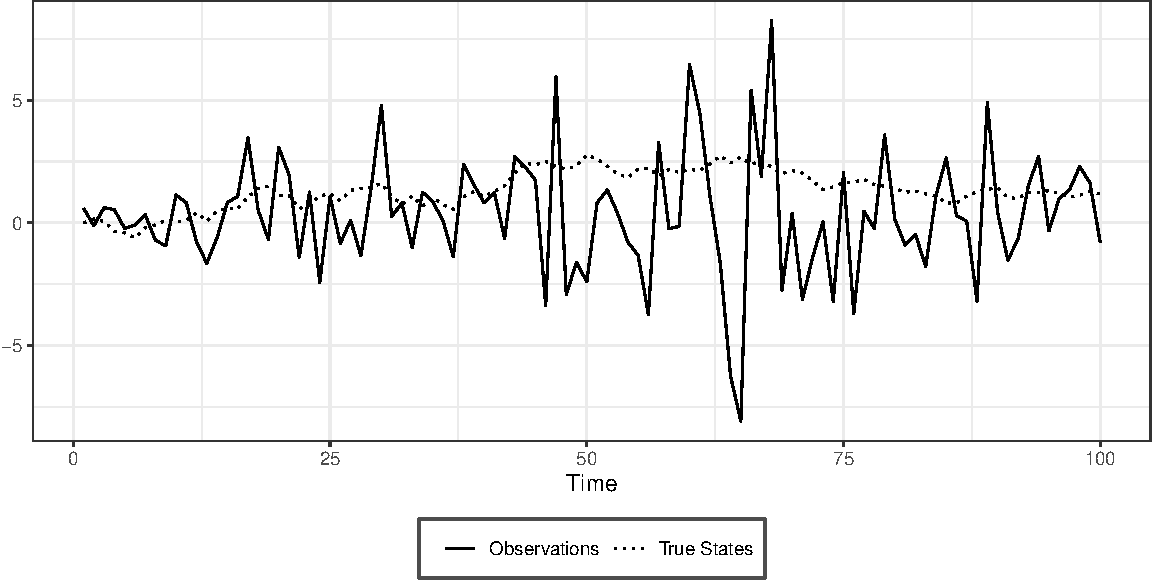
\includegraphics{prova_knit_finale_files/figure-latex/unnamed-chunk-32-1} 

}

\caption{Simulated Stochastic Volatility Model}\label{fig:unnamed-chunk-32}
\end{figure}

We provide both a graphical and a numerical
comparison.\footnote{The sequences of filtered states shown in the graphs are obtained by using filters with 10000 particles.}
From the plots it is hard to say which particle filter provides the best
performances. By and large, BPF, GPF and APF behave similarly, while the
Liu and West filter presents larger credible intervals but at the same
time a higher coverage of the true states.\\
On the other hand, by a RMSE comparison, we see several differences
between the filters. Note that the Guided Particle Filter yields the
lowest RMSE at N=100, and does not improve much even when raising the
number of particles to 100000. Instead, the APF achieves the best
performance in the field when N rises to 10000 and 100000, despite
lagging well behind the BPF and the GPF for the three initial N
thresholds. For the Bootstrap PF, the most significant improvements is
that from N=100 to N=1000. We could then point at the APF as the best
performing and more computationally expensive filter, while the GPF as
the best one at low thresholds (\textit{i.e.} least computationally
expensive, in a way). However, fine margins suggest caution in such
comparative assessments.\\
Rather, we would stress the performance of the Liu and West filter:
indeed, it is apparent that, at least for the first four thresholds,
such filter delivers the worst performance. Even at N=100000, the APF,
the GPF and the BPF are much closer to each other than the LWF, which
still yields the highest RMSE. Such results, in fact, do not come as a
surprise: indeed, note that, while the three best performing filters are
built on a model that perfectly coincides with the true DGP, the Liu and
West filter considers a somewhat misspecified model, which features
additional uncertainty on several parameters. Intuitively, even though
the LWF features some degree of parameter learning, and would then
converge to the correct figures of such parameters, the other filters
``have already learnt'' the true parameters from the
beginning.\footnote{Such difference can be represented as follows. When trying to pin down real valued parameters, the probability that a simple initial guess for each value is correct can be deemed as null. So, in contexts where parameters are unknown, we expect the additional uncertainty featured in the LWF to prove useful, as it can adjust the initial parameters to get closer to the true unknown values. However, in synthetic contexts where we know the DGP, such uncertainty is almost useless.}\\
Finally, notice that in general when the number of particles increases
the accuracy improves; however, significant improvements are not
detected for \(N>10000\), suggesting that such threshold may be a
telling one as regards the convergence of our filters.

\begin{figure}[H]

{\centering 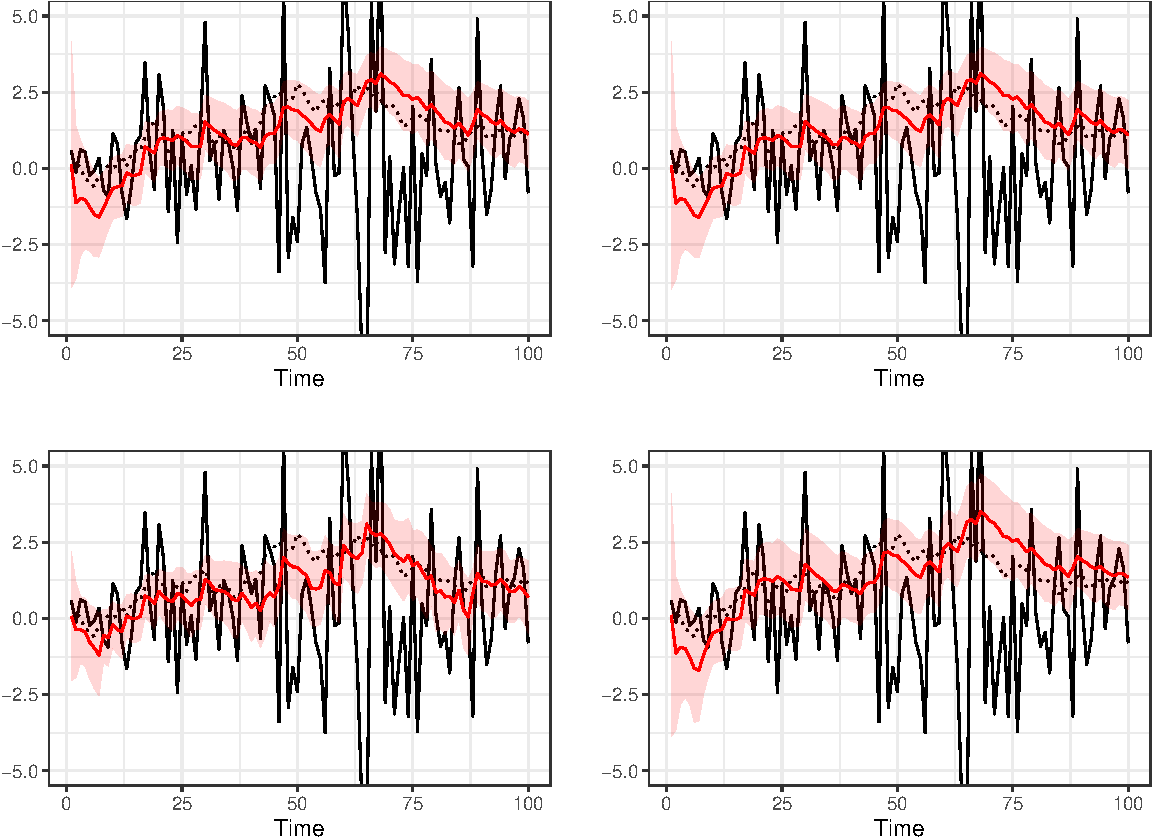
\includegraphics{prova_knit_finale_files/figure-latex/unnamed-chunk-35-1} 

}

\caption{Comparison of filtering strategies for Stochastic Volatility Model. Filtered States with credible interval (in red)}\label{fig:unnamed-chunk-35}
\end{figure}

\chapter{Applications to Stochastic Volatility Models}\label{application_chapter}

\section{Overview}

In the following sections, we will try to replicate some of the analyses
which were previously conducted on synthetic data, generated by a basic
stochastic volatility model; this time, the same model specification and
filters will be used on real data. However, as we will see, real data
require different strategies to evaluate the effectiveness of several
Sequential Monte Carlo techniques. Intuitively, such differences are due
to the fact that now the latent process driving the Hidden Markov Model
is not observed, nor do we know exactly its law of motion.\\
This part of the analysis is structured as follows: section
\textit{fill with the number of the section} provides a review of recent
research in the stochastic volatility literature, including extensions
of the basic specification and the use of particle filters; section
\textit{fill with the number of the section} describes the data which we
employ and the transformations that were applied to them. In section
\textit{fill with the number of the section} we briefly compare the
series of filtered states that are obtained from different particle
filters; moreover, several PFs are compared in terms of computational
cost in approximating the exact filtering distribution implied by our SV
model. Section \textit{fill with the number of the section} features a
forecast comparison between two SV specifications and a model that
assumes constant mean and variance for the financial returns, namely a
forecasting exercise that would not be possible were it not for particle
filtering techniques. In section
\textit{fill with the number of the section} we conclude by employing a
non-parametric measure of realised volatility as a proxy for the latent
volatility process, allowing a RMSE and MAE comparison between filters
which is similar to that of section
\textit{fill with the number of the section} for synthetic data.

\section{A review of Stochastic Volatility models}

In section \textit{fill with the number of the section} a simple
specification of a Stochastic Volatility model was presented and used as
the data generating process of a simulated dataset. Denoting by \(y_t\)
the log returns at time \(t\) and by \(x_t\) the latent volatility
stochastic process, such state-space model was presented as follows,
\begin{align*}
    y_t|x_t & \sim N(0,e^{x_t})\\
    x_t|x_{t-1},\alpha,\beta,\tau^2 & \sim N(\alpha+\beta x_{t-1},\tau^2)
\end{align*}

This specification - which we will employ in this section on a real
dataset - can be deemed as the standard version of the SV model.
Throughout the recent decades, several extensions have been proposed,
mostly (but not exclusively) in the field of financial econometrics. On
the one hand, for simplicity we will stick to the standard version, one
that will suffice for the scope of this work on Sequential Monte Carlo
methods. On the other hand, it is worth mentioning some of these
extensions: indeed, one can rather safely assume that, through their
higher degree of sophistication, such extensions might well improve on
the performance of our standard SV model in the analyses that will
follow.\\
~\\
Stochastic Volatility Models, whose early formulation is commonly
attributed to Taylor (1982, 1986), allow to account for time-varying and
autoregressive volatility in financial returns, posing themselves as a
valid alternative to ARCH (Engle 1982) or GARCH (Bollerslev 1986) models
in dealing with non-constant volatility. Kim, Shephard and Chib (1998)
define the canonical model for regularly spaced data as \begin{align*}
    y_t & = \psi e^{\frac{x_t}{2}}\epsilon_t\\
    x_{t+1} & = \mu+\beta(x_t-\mu)+\tau \eta_t\\
    x_1|\sigma,\beta & \sim  N\Big(\mu,\frac{\sigma^2}{1-\beta^2}\Big)\\
    \epsilon_t & \sim N(0,1)\\ 
    \eta_t & \sim N(0,1)
\end{align*} where the log volatility \(x_t\) is assumed to follow a
stationary process (\(|\beta|<1\)), \(\psi\) is a constant scaling
factor, \(\beta\) is the persistence in the volatility and \(\tau\) is
the volatility of the
log-volatility.\footnote{For identifiability reasons, either $\psi=1$ or $\mu=0$. Kim, Shephard and Chib (1998) prefer $\psi=1$.}
Most importantly, \(\epsilon_t\) and \(\eta_t\), the Gaussian white
noise processes that drive the canonical model, are assumed to be
uncorrelated. This latter assumption justifies another definition of
this specification, namely ``discrete SV model without
leverage''.\footnote{Note that in this review we do not focus on continuous time SV models. In fact, such models have attracted a considerable amount of research in financial econometrics and mathematical finance, especially after Hull and White (1987) considered stochastic volatility for option pricing. Arguably, the most influential model was then proposed for option pricing by Heston (1993), a SV model with leverage effects and square root diffusion driving volatility. Diffusion-based SV models enjoyed increasing popularity, see for example Barndorff-Nielsen and Shephard (2001), or Christoffersen et al. (2010), who investigate alternatives to the entrenched affine square root SV model.  Eraker (2004) proposed a SV model with correlated jumps in prices and volatility, extending Heston's model, while Comte and Renault (1998) extended Hull and White's model as to feature long memory properties. More recently, Gatheral et al. (2018) further built on Comte and Renault's fractional SV model to propose the popular "rough volatility models" (see also Friz et al., 2021).}\\
In order to accommodate for leverage effects, namely capture the
increase in volatility that follows a drop in the returns, the model can
extended as in Omori et al.~(2007), \begin{align*}
    y_t & = e^{\frac{x_t}{2}}\epsilon_t\\
    x_{t+1} & = \mu+\beta(x_t-\mu)+\eta_t\\
    \begin{pmatrix}
       \epsilon_t \\
       \eta_t
    \end{pmatrix} \Big|\rho,\tau & \overset{i.i.d.}{\sim}  N_2(\mathbf{0},\Sigma), \ \Sigma=
    \begin{pmatrix}
       1 & \rho\tau \\
       \rho\tau & \tau^2
    \end{pmatrix}
\end{align*} where \(\rho<0\) captures the negative correlation. Such
specification, which can be referred to as ``discrete SV model with
leverage'', captures the asymmetric response of volatility to returns of
different signs, so that similar specifications are sometimes also
deemed as ``asymmetric SV models'' (e.g.~Harvey and Shephard 1996, Mao
et al.~2020).\\
Note that so far the assumptions on \(\epsilon_t\) and \(\eta_t\)
implied that the returns are conditionally normally distributed. The
discrete time SV models can also be extended to allow for heavy-tailed
or asymmetric conditional returns distributions: symmetric or skewed
Student-\(t\), Generalised Hyperbolic (GH) distribution, Generalised
Error Distribution (GED) and scale mixtures of normals feature as
popular choices (Kim and Stoffer 2008, Nakajima and Omori 2012, Mao et
al.~2020). In fact, SV with heavy tailed return distributions were shown
to better meet empirical regularities like the leptokurtic distribution
of the returns and slowly decaying autocorrelation functions of the
squared returns (Liesenfeld and Jung 2000).\\
Assuming that \(\epsilon_t\) follows a Student-\(t\) distribution, and
exploiting the fact that \(\epsilon_t\) can then be written as
\(\lambda_t^{-1/2}\zeta_t\), where \(\zeta_t \sim N(0,1)\) and
\(v\lambda_t \sim \chi^2_v\) (Harvey et al.~1994, Chib et al.~2002), we
have the following SV model with both fat tails and leverage effect
(Jacquier et al., 2004), \begin{align*}
    y_t & = e^{\frac{x_t}{2}}\lambda_t^{-1/2}\zeta_t\\
    x_{t+1} & = \alpha + \beta x_t + \eta_t\\
    \begin{pmatrix}
       \zeta_t \\
       \eta_t
    \end{pmatrix} \Big|\rho,\tau & \overset{i.i.d.}{\sim}  N_2(\mathbf{0},\Sigma), \ \Sigma=
    \begin{pmatrix}
       1 & \rho\tau \\
       \rho\tau & \tau^2
    \end{pmatrix}\\
    v\lambda_t & \sim \chi^2_v
\end{align*} To capture other elements of the behaviour of financial
data, several other extensions have been proposed. For example, SV
models have been extended to include conditional heteroskedasticity in
the mean returns (Koopman and Hol Uspensky 2002) to capture potential
volatility feedback effects, or to feature autoregressive moving average
innovations (Chan 2013, Zhang et al.~2020), allowing better goodness of
fit and out-of-sample
forecasts.\footnote{Dimitrakopoulos and Kolossiatis (2020) note that "the moving average component, the leverage effect and the conditional heteroscedasticity in mean have been considered separately in the stochastic volatility literature" and provide two specifications, one featuring an MA component and leverage effects, the other an MA component and conditional heteroskedasticity in mean.}
\footnote{Other extensions, though ones for which we do not report the specifications, feature modelling the latent volatility process $x_t$ as an ARFIMA process (Long Memory Stochastic Volatility model, Breidt et al. 1998) or as governed by a first-order Markov process (Markov Switching Stochastic Volatility model, So et al. 1998). Recently, Luo et al. (2018) incorporated neural networks in the stochastic volatility model (Neural Stochastic Volatility Model), while Xu and Chen (2021) employ deep learning models (Deep Stochastic Volatility Model).}
The model proposed by Koopman and Hol Uspensky is specified as
\begin{align*}
    y_t & = \nu_t+\psi e^{\frac{x_t}{2}}\epsilon_t\\
    \nu_t & = a+by_{t-1}+d\psi^2e^{x_t}\\
    x_t & = \beta x_{t-1}+\tau \eta_t\\
    \begin{pmatrix}
       \epsilon_t \\
       \eta_t
    \end{pmatrix} & \overset{i.i.d.}{\sim}  N_2\Big(\mathbf{0},\begin{pmatrix}
       1 & 0 \\
       0 & 1
    \end{pmatrix}\Big)
\end{align*} while the state space representation of the ARMA(p,q)-SV
framework, as in Zhang et al.~(2020), reads \begin{align*}
    y_t & = \nu_t + \gamma_t\\
    \gamma_t & =\phi_1\gamma_{t-1}+...+\phi_p\gamma_{t-p}+u_t+\varphi_1 u_{t-1}+...+\varphi_q u_{t-q}\\
    u_t|x_t & \sim N(0,e^{x_t})\\
    x_{t} & = x_{t-1}+ \eta_t\\
    \eta_t|\tau & \sim N(0,\tau^2)
\end{align*} where the error terms \(u_t\) and \(\eta_t\) are
independent across all leads and lags, while \(\nu_t\) follows an
unspecified time-varying process.\\
~\\
Interestingly enough, the path along which the SV models evolved
coincides with that suggested by optimal portfolio findings. Johannes,
Korteweg and Polson (2014) found that, in order to generate
statistically significant portfolio improvements in a Bayesian learning
problem, the model employed by the investor should incorporate both
time-varying expected returns and stochastic volatility: indeed, either
of these features alone did not lead to statistically significant gains
with respect to employing models with time-constant expected returns and
volatility.\footnote{One could then argue that caution is needed when employing basic specifications of stochastic volatility models. For instance, Poon and Granger (2005) found that historical volatility and ARCH models both achieved better volatility forecasting performance than SV models. Similarly, Allen and McAleer (2020, see also Allen, 2020) found that, using realised volatility as benchmark, neither the canonical SV model or a GARCH(1,1) specification could forecast better than a simple form of historical volatility model.}\\
~\\
Finally, before moving to the application of Sequential Monte Carlo
techniques to a SV model, we conclude by going through some references
for the Bayesian analysis proposed for such models. Starting from the
seminal work of Jacquier et al.~(1994), the use of MCMC methods has
become increasingly popular for parameter estimation and smoothing
exercises in SV models (e.g.~Kastner 2019, presenting the R package
\textit{stochvol} for Bayesian parameter estimation, and Chopin and
Papaspiliopoulos 2020, who use MCMC to sample from the smoothing
distribution of a SV model). As regards filtering exercises, the
adoption of particle filters was rather
rapid:\footnote{Actually, SV models are now often used as straightforward applications of particle filters on non-linear state space models, see for example Andrieu et al. (2010), Douc et al. (2014) or Chopin and Papaspiliopoulos (2020).}
indeed, latent volatilities in Kim et al.~(1998) were already filtered
by employing the particle filter suggested in Pitt and Shephard (1999),
paving the way for subsequent applications (\textit{inter alia}) in Chib
et al.~(2006), Omori et al.~(2007), Kim and Stoffer (2008) and Nakajima
and Omori (2012).\\

\section{Data Description}

As previously mentioned, we will analyze the behaviour of the described
filtering tools associated to a simple stochastic volatility model. In
particular, we are evaluating the performance of such model on real
data. For the observable process, namely financial returns in the SV
model, we consider the continuously compounded daily returns (also
called logarithmic returns) of three indices, S\&P500, DOW JONES and
STOXX50, in a time interval from June 1st, 2017 to May 30th, 2021. From
these, we estimate the daily volatility, as computed by the model.

The indices have been selected as representatives of the global economic
trends in the US and EU markets. Specifically, the S\&P500 is a
market-capitalization-weighted stock-price index tracing the performance
of the 500 largest companies listed on US stock exchanges (NYSE and
Nasdaq Exchange). The DOW JONES, instead, is a price-weighted
stock-market index and accounts for the 30 major companies listed on US
stock exchanges, characterized for being ``blue-chip''. Also the EURO
STOXX 50 follows bluce-chip stocks representing leading firms in regions
of the Eurozone.\\

The three plots below represent the time series of the log returns
calculated for the three indices during our period of interest. In
particular, each series is a sequence of daily observations representing
the logarithm of the ratio between the closing price of the index for a
given day and the closing price of the day before.

\begin{figure}[H]

{\centering \includegraphics{prova_knit_finale_files/figure-latex/unnamed-chunk-38-1} 

}

\caption{Close to close percentage log returns, 3 indices}\label{fig:unnamed-chunk-38}
\end{figure}

At a first visual inspection, we can see a common behaviour in the
volatility of all three indices. Especially, it is worth pointing out
the similarity between the pattern of DJI and that of S\&P500
(especially in terms of peaks), which both differ from the STOXX50E,
presumably because the first two describe the US stock market, while the
last index describes the European one. For example, a difference that
can be seen by having a glance at the plots is that the US indices log
returns displays differences in fluctuation magnitude across different
periods that are more marked than for the EU index, for which log
returns display, in general, wider fluctuations. Anyways, what stands
out the most in all three plots is the very wide fluctuations present
from February - March 2020 to around September 2020, which, very
intuitively, are connected with the Covid-19 Pandemic Crisis.

\begin{longtable}[t]{lccc}
\caption{\label{tab:unnamed-chunk-39}Summary statistics, close to close percentage log returns}\\
\toprule
  & S\&P500 & Dow Jones & STOXX50E\\
\midrule
Mean & 0.05581 & 0.05002 & 0.01229\\
Standard Deviation & 1.32564 & 1.38510 & 1.22951\\
\bottomrule
\end{longtable}

As regards the series that we will employ in section
\textit{fill with the number of the section}, namely the series of
realised volatilities which we will employ as a proxy for the true
latent volatilities, the data were retrieved from the Oxford-Man
Institute's Realized Library, which provides several different daily
non-parametric measures of past
volatility.\footnote{Such class of measures will be better presented in section \textit{fill with the number of the section}, when reviewing the use of realised volatility estimators as proxies for latent volatilities.}
We consider a proper rescaling of the \textit{rv5} series, \textit{i.e.}
model-free daily volatility estimates based on 5 min intraday return
intervals. Also in this case, the chosen interval spanned from June 1st,
2017 to May 30th, 2021. The plots below represent the realized
volatility in the period of interest for all the three
indices.\footnote{In the graph, the series $rv5$ is rescaled as specified in the upcoming section: we took the square root of each value, which is a daily variance measure, and multiplied it by 100.}
As usual, they show a rather similar pattern across all three indices,
identifying peaks corresponding to periods of higher uncertainty (in
particular referring to the 2020 Covid-19 Crisis outbreak and its impact
over time). Once more, there is great similarity between the series for
the DJI and the one for the S\&P500, while the series of the STOXX50E
appears slightly different, in terms of peaks.

\begin{figure}[H]

{\centering \includegraphics{prova_knit_finale_files/figure-latex/unnamed-chunk-40-1} 

}

\caption{Rescaled realised daily volatility, 3 indices}\label{fig:unnamed-chunk-40}
\end{figure}

\subsection{Rescaling the data}

When specifying the parameters of a stochastic volatility model, one
should clarify whether the series of observed financial returns is one
of log returns or of percentage log returns. Indeed, let \(y_t\) denote
the returns at time \(t\), so that a basic SV specification would
prescribe \(y_t|x_t\sim N(0,e^{x_t})\): clearly, for each period \(t\),
\(e^{x_t}\) needs to be higher to replicate the observed
\textit{percentage} log return rather than the observed log return. This
implies that the latent volatility \(x\) should fluctuate around higher
values when using percentage log returns as \(y_t\). This feature, when
adopting the aforementioned canonical SV model as defined in Kim et
al.~(1998), would be represented by a higher \(\mu\). For example, as
noted in Kastner (2019), daily log returns often have a variance of
0.0001 or less, which implies that \(\mu\) should lie somewhere around
\(\ln(0.0001)\approx -9\); instead, when considering daily percentage
log returns, one then has a variance of 1, so that \(\mu=\ln(1)=0\). In
other terms, one might end up with a basic specification of the SV model
when (roughly) calibrating the parameters of the canonical model on a
wider set of financial returns.

Note that rescaling the log returns has analogous implications for the
section in which we employ measures of realised volatility as a proxy
for the latent volatility process. Let us denote by \(rv5_t\) the daily
realised variance at time \(t\), which we obtain from the \textit{rv5}
series provided in the Oxford-Man database. Now, note that in a SV
framework one should not directly compare \(rv5_t\) to \(x_t\), as
\(rv5_t\) can be rather seen as an estimate of the variance of the log
returns at time \(t\), \textit{i.e.} of \(e^{x_t}\) in the SV
model.\footnote{See for example Guidolin and Pedio (2021), who employ $rv10$, another measure of realised volatility provided in the Oxford-Man Library, as a proxy for the latent conditional variance of the daily log returns on the FTSE100 index.}
Moreover, by construction of \(rv5_t\), the comparison should feature a
SV model where the log returns did \textit{not} undergo the percentage
transformation.\footnote{Indeed, this estimator is based on the sum of 5-minute intra-day squared returns: such returns are computed as the difference between the opening and closure price in an interval.}
Thus, in order to achieve a common scale with the percentage log
returns, we need to multiply \(rv5\) by \(100^2\). To ease the
interpretation and representation of the comparison between differently
approximated filtering distributions, we finally take the square root of
the rescaled \(rv5\), so that we compare it to \(e^{x_t/2}\).

\section{Comparing the filters}

In this section the different particle filter techniques we discussed in
earlier sections will be employed to approximate the filtering
distribution that springs from a simple SV model applied to a real
dataset. First, we provide a qualitative comparison between the filters,
basing on visual analysis of the (approximated) filtering distributions.
Subsequently, we move to a more quantitative approach, in order to
assess the quality of the approximations as the number of particles
increases. In a way, while in the first part most filters can be rather
confidently assumed to be close to convergence, the second subsection
will hint at possibly different computational costs across the competing
filters.\\
Before moving to such analyses, it is worth mentioning that not all the
filters we employ approximate the same filtering distribution
\(p(x_t|y_{1:t},\psi)\), where \(\psi\) is a vector containing the
parameters of the model. Indeed, the Liu and West filter actually
approximates the distribution of a slightly different SV model, one that
assumes an additional hierarchical level, \begin{align*}
y_t|x_t & \sim N(0,e^{x_t})\\
x_t|x_{t-1},\alpha,\beta,\tau^2 & \sim N(\alpha+\beta x_{t-1},\tau^2)\\
x_0 & \sim N(0,100)\\
\alpha & \sim N(\gamma,\zeta)\\
\beta & \sim N(\pi,\phi)\\
\tau^2 & \sim IG(\nu/2,\lambda \nu/2)
\end{align*} where \(\gamma\),\(\zeta\),\(\pi\),\(\phi\),\(\nu\) and
\(\lambda\) are assumed to be
known.\footnote{In these empirical applications we keep the values of the parameter we employed in the synthetic data part, see section \textit{fill with the number of the section}}.\\

\subsection{Visual Analysis after Filtering}

We now offer a preliminary comparison of the various filtering methods,
based on a visual analysis of graphs representing, for each index, the
time-varying volatility of the observations, obtained through the
application of the different filtering techniques explored in the
theoretical analysis. Plots that are compared represent the sequence of
percentage log returns for a given index (the observations, in gray) and
the sequence of filtered volatilities calculated using filtered states
(in red) obtained through a specific filtering technique indicated in
the caption of the
plot.\footnote{Such filtered volatilities are obtained as follows. For each $t$, let us denote by $\mu_t$ the mean of the generated particles; the filtered volatility is then defined as $e^{\mu_t}$. Note that the number of particles was set at 10000 for each filter: the conclusion of the next section will come back to such a choice.}\\

First, a general point is that the sequence of percentage log returns
are different across the three indices. The reasons why this holds can
be associated with the index-construction method and the characteristics
of the economy and industrial setting it represents (SEE SECTION X). In
particular, as previously noticed, there are extensive similarities
between the DOW JONES Index and the S\&P500, which can be visualized
when looking at the percentage of log returns in the corresponding
plots, since both are describing the US Economy. However, the STOXX50E
differs quite extensively, especially in the different sensitivity to
the Covid-19 Crisis and its consequences, representing the European
Economy. Aside from this note, the considerations expressed below on the
sequences ``filtered
volatilities''\footnote{Per ora nei grafici c'è scritto "Filtered States", verrà corretto.}
for the various techniques hold almost uniformly for all the three
indices. Therefore, in the next paragraph we will be referring to the
set of plots pertaining to one specific index (which could be any of the
three).\\

Generally speaking, note that, the sequence of ``filtered volatilities''
obtained from any of the filtering techniques follows roughly similar
paths across all the plots. Unsurprisingly, the filtered volatility
appears wider in periods corresponding to wider fluctuations of the
percentage log returns and lower in periods corresponding to smaller
such fluctuations. For example, all sequences of filtered volatilities
show peaks corresponding to the higher fluctuations due to the 2020
Covid-19 Crisis outbreak and the consequent increases in uncertainty for
the later periods.\\

When focusing the attention on specific filters, first we can discuss
the effect of resampling. Indeed, in the plot referring to the
Sequential Importance Sampling procedure, the sequence of filtered
volatilities is not able to reproduce the peaks as in with other
filters, but also is characterized by collapsing confidence intervals.
This is because :::::::\\
Then, if we instead look at the filtered volatilities obtained with
resampling, we can appreciate how the filtered sequences for the
Basic,\footnote{By this name, we refer to a particle filter that features no adaptive resampling; rather, resampling is conducted at each step of the algorithm.}
Bootstrap, Auxiliary and Optimal Kernel Guided particle filters give
rather analogous results, with no differences appearing at a first
visual
inspection.\footnote{Except for the Auxiliary Particle filtered sequence of volatilities, showing a slightly higher peak corresponding to the greatest volatility fluctuation in 2020, if compared to other filters in this subset. This is still valid for all three indices.}\\
However, the sequence of filtered volatilities obtained by applying the
Liu and West filter is clearly different from the others. Indeed, it
shows a ``more detailed'' sequence of states (in the sense of the
sequence of filtered volatilities being less smooth) and also a higher
peak for the wide fluctuation corresponding to the 2020 Covid Crisis
outbreak. Therefore, we may expect that, compared to other filtering
techniques, it can provide a better representation of the data. This is
because \ldots{}
\textit{Potremmo parlare di maggiore sensibilità alle oscillazioni dei prezzi, o simili}

\subsection{Quality of approximation}

Since we do not have access to the exact filtering distribution of the
SV model, when assessing how rapidly different particle filters converge
to it, we actually need to approximate even such target distribution as
to have a benchmark.\\
Fortunately, convergence results about particle filters ensure that when
the number of particles diverges, the approximation converges to the
target
distribution.\footnote{Molto probabilmente la frase formulata così non è formalmente corretta...bisognerebbe fare riferimento alla sezione sulla convergenza. Inoltre, va chiarito il punto della "doppia convergenza".}
Thus, we run one of the particle filters with a very large number of
particles, and assume that such approximation is close enough to the
target to be used itself as the distribution the filters should tend
to.\\
With such a benchmark, we can then compare how different filters
approach it as the number of particles increases. We employ the Root
Mean Squared Error and the Mean Absolute Error to measure discrepancies
from the benchmark. Note that the Liu and West filter can not be
included in such an analysis: trivially, the comparison assumes that the
competing algorithms are approximating the same target
distribution.\footnote{For an analogous reason, we do not need to conduct this analysis on all the indices, but we can rather focus on one, the SP500. Indeed, what matters in this section is not how well the model fits the data, but rather how different algorithms approach the same distribution yielded by the same model on a given set of data.}

We start by running the Bootstrap particle filter with N=50000, setting
it as the benchmark. In table XX we report the RMSE and MAE measures one
obtains by comparing the mean of the particles generated at each step by
the Bootstrap PF with N=50000 and the
mean\footnote{As a possible limitation of our exercise, here we do not consider in detail the variance of such generated particles. Nevertheless, one can get at least an idea of the differences in the generated variances by comparing the confidence intervals that will be shown in the graphs below. Unsurprisingly, it will be apparent that including a resampling step is essential to avoid a collapsing effective sample size.}
of the particles generated by other particles filters with N equal to
10, 100, 1000, 5000 or
10000.\footnote{We consider 5 algorithms: a Bootstrap PF, a Guided PF (with the optimal proposal kernel), an Auxiliary PF, a "Basic PF" and a Sequential Importance Sampling alogrithm. By "Basic PF" we refer to a Bootstrap PF that features resampling at each step, whereas resampling never happens in the SIS algorithm: one can then consider these 2 algorithms as extreme cases of an adaptive resampling algorithm, namely one that features resampling when $ESS$ is non negative (\textit{i.e.} always) or when $ESS<0$ (\textit{i.e.} never). In this sense, we use the shorthand "particle filters" when referring to all the 5 algorithms.}

\begin{longtable}[t]{lcccccc}
\caption{\label{tab:unnamed-chunk-42}RMSE and MAE, Bootstrap PF 50000 particles}\\
\toprule
  & N & BPF & GPFOPT & APF & BAPF & SIS\\
\midrule
RMSE & 10 & 0.42331 & 0.36853 & 0.54784 & 0.55959 & 0.91686\\
RMSE & 100 & 0.15689 & 0.15094 & 0.24044 & 0.23488 & 1.10551\\
RMSE & 1000 & 0.06901 & 0.07669 & 0.08878 & 0.10295 & 0.62505\\
RMSE & 5000 & 0.03817 & 0.03568 & 0.05742 & 0.06110 & 0.62004\\
RMSE & 10000 & 0.03045 & 0.02709 & 0.04296 & 0.05151 & 0.51189\\
\addlinespace
MAE & 10 & 0.28078 & 0.27961 & 0.43103 & 0.43779 & 0.72753\\
MAE & 100 & 0.09658 & 0.09624 & 0.17570 & 0.18394 & 0.91799\\
MAE & 1000 & 0.03312 & 0.03697 & 0.05539 & 0.06726 & 0.49718\\
MAE & 5000 & 0.01889 & 0.01665 & 0.03186 & 0.03448 & 0.44753\\
MAE & 10000 & 0.01456 & 0.01423 & 0.02449 & 0.02726 & 0.40636\\
\bottomrule
\end{longtable}

As we can see, almost every filter shows dramatic improvement already
when passing from 10 particles to 100 particles, while the performance
of the SIS algorithm actually gets worse. With N=10 or N=100, the
Bootstrap PF and the Guided PF (with optimal proposal kernel) emerge
quite clearly as the best performing filters; however, no conclusion
should be drawn at this stage, as the large errors seem to suggest quite
a wide margin from improvement even for the best performing filters.\\
As it turns out, such suggestion is confirmed by running the algorithms
with N=1000. Passing from 100 to 1000 particles more than halves the
RMSEs across the 5 competing filters, with even more pronounced gains in
the MAEs; at N=1000, the Bootstrap and the Guided particle filters still
hold their lead over the rest of the field, keeping a shrinking hedge
over the Auxiliary PF, which shows most impressive gains when passing
from 100 to 1000 particles. Further sizable gains for every filter,
except for the SIS algorithm, are observed when increasing the number of
particles to 5000, a level at which both the RMSE and the MAE agree on a
slight hedge of the Guided and the Bootstrap filters over the Auxiliary
and the Basic PFs.\\
Nevertheless, we would argue that already for N=5000, but even more
clearly for N=10000, the difference between the Bootstrap, the Guided
and the Auxiliary particle filters is so small that none of these
filters can be straightforwardly chosen over the others, a figure which
visual inspection of the graphs below can confirm. Interestingly enough,
no gains seem to arise from resampling at each step with respect to
adaptive resampling (note that the Basic PF is preferred to the APF only
once, by the RMSE), whereas the need of some degree of resampling is
apparent, as shown by the awful performance of the SIS algorithm with
any number of particles. Moreover, the RMSE and the MAE show infrequent
disagreement, delivering a rather clear picture of the comparison.

Now, one might argue that the relative performance of the filters is
influenced by the choice of the Bootstrap filter as the benchmark
algorithm when run with N=50000: intuitively, if the convergence phase
were not reached, the Bootstrap filter (which did in fact come out as
one of the best performing algorithms) would clearly find it easier to
replicate the benchmark we
set.\footnote{Note that all the filters, including the BT filter run with 50000 particles, shared the same seed in the $R$ software, ruling randomness out of these considerations.}\\
As a robustness check, we thus conduct the same analysis employing the
Auxiliary Particle Filter as the benchmark, keeping the number of
particles set to 50000 as for the benchmark BT filter.

\begin{longtable}[t]{lcccccc}
\caption{\label{tab:unnamed-chunk-44}RMSE and MAE, Auxiliary PF 50000 particles}\\
\toprule
  & N & BPF & GPFOPT & APF & BAPF & SIS\\
\midrule
RMSE & 10 & 0.40549 & 0.34950 & 0.53237 & 0.54597 & 0.91038\\
RMSE & 100 & 0.13510 & 0.14209 & 0.22243 & 0.22398 & 1.10156\\
RMSE & 1000 & 0.04145 & 0.06874 & 0.07796 & 0.07692 & 0.61504\\
RMSE & 5000 & 0.02847 & 0.04922 & 0.03931 & 0.05230 & 0.61176\\
RMSE & 10000 & 0.03048 & 0.03337 & 0.02648 & 0.02411 & 0.50547\\
\addlinespace
MAE & 10 & 0.27266 & 0.26941 & 0.42151 & 0.42909 & 0.72112\\
MAE & 100 & 0.08540 & 0.09034 & 0.16691 & 0.17484 & 0.91468\\
MAE & 1000 & 0.02329 & 0.03532 & 0.05105 & 0.05753 & 0.48959\\
MAE & 5000 & 0.01756 & 0.02410 & 0.02662 & 0.03275 & 0.44195\\
MAE & 10000 & 0.01417 & 0.01718 & 0.01974 & 0.01742 & 0.40221\\
\bottomrule
\end{longtable}

Using the APF as the benchmark does not deliver a different picture than
the one we previously had. Leaving the SIS algorithm aside (whose
analogous performance comes as no surprise), it is interesting to note
how once again the Auxiliary particle filter actually fares worse than
the Bootstrap and the Guided PFs at 10, 100 and 1000 particles.\\
Its performance ameliorates dramatically at N=1000, while at N=5000 the
halving of its RMSE and MAE even allows the APF to overtake the Guided
PF, though falling short of the Bootstrap PF. At N=10000 both the Basic
PF and the APF achieve lower RMSEs than the Bootstrap and the Guided PF,
even though the MAE criterion still selects the Bootstrap as the closest
to the target distribution.\\
Interestingly, this time the performance of the Bootstrap filter worsens
when N is increased from 5000 to 10000 (both according to RMSEs and
MAEs, whose disagreements, once again, are overall infrequent). Such
evidence suggests that, even at very large (yet finite) values of N,
some difference between the approximated filtering distributions still
persists across our particle filters.\\

\begin{longtable}[t]{lcc}
\caption{\label{tab:unnamed-chunk-46}Discrepancy between Bootstrap and Auxiliary PFs}\\
\toprule
  & RMSE & MAE\\
\midrule
N=50000 & 0.04408 & 0.01668\\
N=100000 & 0.03576 & 0.01476\\
\bottomrule
\end{longtable}

In fact, by comparing the two benchmark approximations with N=50000, we
can see that, for example, the Bootstrap PF run with N=10000 is closer
to the benchmark APF than the benchmark BT is, or that the RMSE ranks
the APF with N=10000 as closer to the the benchmark BT than the APF with
N=50000, mildly pointing at a theoretically-unsound difference between
the limiting distributions of the filters. Nevertheless, now the RMSE
and MAE do not deliver unanimous verdicts, nor the differences seem
large enough to back extreme claims. And, conveniently, running the
Auxiliary and the Bootstrap filters with 100000 particles testifies a
shrinking difference between the approximations - at increasingly large
computational costs, though.\\

Overall, we should not overplay tiny
differences.\footnote{Indeed, the mere extent of such difference also depends on the real dataset which is used for the comparison, implying different target distributions. For example, running the same experiment using the STOXX50E dataset, we have even smaller differences between the filters at N=50000, with RMS difference between the Bootstrap and the Auxiliary equal to 0.01236279 and mean absolute difference equal to 0.008028818.}
Rather, we prefer to stress the points that emerged from both benchmark
analyses and we can therefore support quite confidently.\\
First, if on the one hand it is clear that some degree of resampling is
essential, on the other we found no gains from resampling at each
period.\\
Second, when the number of particles is set at 5000 or more, neither
benchmark could single out an algorithm that clearly outperformed the
others, when restricting the analysis to procedures that feature
adaptive resampling rules.\\
Third, when the number of particles was set to 10, 100 or 1000, the
Bootstrap particle filter and the Guided particle filter with optimal
proposal kernel significantly emerged as the best performing algorithms
for our SV model, suggesting that their computational cost is lower than
that of the Auxiliary particle filter, which needed more particles to
``get rolling''.\\
Finally, some discrepancy between different approximations persisted
even when the number of particles was set to 50000 or 100000. However,
the narrow extent of the RMSEs and MAEs with respect to both benchmarks
supports the idea that at N=10000 the best-performing algorithms have
already entered the phase of convergence. Even in light of these
markedly more computationally expensive benchmarks, we then choose
N=10000 as the number of particles which we routinely employ in this
empirical application.

\section{Comparing Constant and Stochastic Volatility Models of Equity Returns}

In this section, we apply the particle filter in a model-comparison
exercise, ultimately underlining the importance of taking stochastic
volatility into account in modeling equity returns. We follow XX,
comparing density forecasts through relative predictive and cumulative
likelihoods.

We analyze a dataset of log close-to-close returns of the S\&P500, from
2017 to 2021. Consider a stochastic volatility model \[
\mathcal{M}_{SV}:\begin{array}{lc}
r_{t}=\alpha_{r}+\sigma_{r,t}\cdot v_{t}\\
\log\sigma_{r,t}^{2}=\alpha_{\sigma}+\beta_{\sigma}\cdot\log\sigma_{r,t-1}^{2}+\sigma_{\sigma}\cdot w_{t}
\end{array}\ (v_{t},w_{t})\sim\mathcal{N}_{2}(\boldsymbol{0},I_{2})
\]

and a constant volatility iid model \[
\mathcal{M}_{CV}:(r_{t})\overset{iid}{\sim}\mathcal{N}(\alpha,\sigma^{2}).
\]

We calibrate the model parameters using the whole sample, and proceed by
setting the return mean of both models to equal the sample mean,
\(\sigma^{2}\) equal to the return variance, and the parameters of the
volatility equation in \(\mathcal{M}_{SV}\) by running an \(AR(1)\)
regression of the log squared residuals.

In order to compare the predictive performance of the two, we compare
the cumulative log likelihood of the observed returns up to time \(t\)
given the considered model. In formulas, the cumulative likelihood can
be computed as \[
p(y_{1:t}|\mathcal{M}_{i})=\prod_{s=0}^{t-1}p(y_{s+1}|y_{1:s},\mathcal{M}_{i}),i\in\{SV,CV\},
\]

adopting the convention \(y_{1:0}=\emptyset\). This is trivial to obtain
in the iid case; considering the stohastic volatility model, the
predictive likelihoods can be derived as

\[
p(y_{t+1}|y_{1:t},\mathcal{M}_{SV})=\int p(y_{t+1}|\sigma_{r,t+1},y_{1:t},\mathcal{M}_{SV})p(\sigma_{r,t+1}|y_{1:t},\mathcal{M}_{SV})d(\sigma_{r,t+1})
\] \[
=\int p(y_{t+1}|\sigma_{r,t+1}\mathcal{M}_{SV})p(\sigma_{r,t+1}|y_{1:t},\mathcal{M}_{SV})d(\sigma_{r,t+1})
\]

Whereas the emission distribution
\(p(y_{t+1}|\sigma_{r,t+1}\mathcal{M}_{SV})\) is known, we approximate
the predictive state distribution
\(p(\sigma_{r,t+1}|y_{1:t},\mathcal{M}_{SV})\) with weighted particles
obtained with particle filtering.

Figure XX reports the time series of the cumulative log-likelihood given
the constant volatility model \(\mathcal{M}_{CV}\) relative to the one
given \(\mathcal{M}_{SV}\), obtained as
\(\log p(y_{1:t}|\mathcal{M}_{CV})-\log p(y_{1:t}|\mathcal{M}_{SV})\).
Notice that the first difference of this series is the relative
log-likelihood of the incoming observation,
\(p(y_{t}|y_{1:t-1},\mathcal{M}_{CV})-p(y_{t}|y_{1:t-1},\mathcal{M}_{SV})\).

\begin{figure}[H]

{\centering 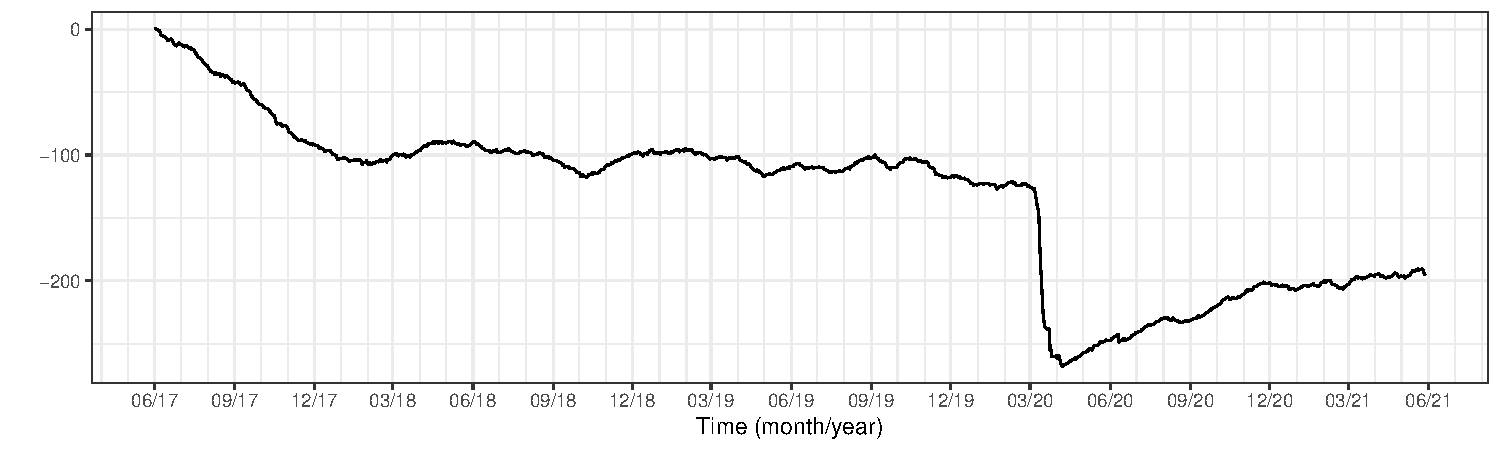
\includegraphics{prova_knit_finale_files/figure-latex/cll_plot-1} 

}

\caption{Relative log-likelihood}\label{fig:cll_plot}
\end{figure}

Overall, this analysis shows how a model with stochastic volatility is
better at describing and predicting the considered time-frame of S\&P500
returns. As can be seen from the graph and perhaps unsurprisingly, the
density forecast given the stochastic volatility model represents a
particularly significant improvement in the period of extreme values of
returns in March 2020.

\section{Realised volatility as benchmark}

In section XX we compared several filtered distributions, briefly
pointing out three main behaviours, namely that of the SIS algorithm,
that of the Liu and West particle filter and that of the remaining
filters. However, we did not have metrics that could help us clearly
point at one behaviour as the closest to reality. In this section, we
will employ realised volatility as one such metric.\\
A realised volatility measure - the realised variance based on 5 min
intraday return intervals (\(rv5\) series in the Oxford-Man Realized
Library) - will be used as a proxy for the latent volatility process
driving the log returns on the 3 indices presented in the earlier
sections. As we previously mentioned, a transformation is needed as to
compare filtered states and realised volatility, namely one turning both
into estimates of the standard deviation of the percentage log returns.
For each \(t\), \(rv5_t\) is then turned into \(rv5_t^{0.5}*100\), while
\(e^{x_t/2}\) (where \(x_t\) is the filtered state) is computed by
taking the mean of the generated particles and then applying the
\(exp(\cdot /2)\) transformation.\\
Throughout this section, we will deem as the best performing algorithm
that coming closest to the proxy, either ``literally'' in a graphical
framework or in a Root Mean Squared Error or Mean Absolute Error sense.
Clearly enough, this approach builds on the assumption that realised
variance is indeed a good proxy for latent volatility in real financial
series.\\

A considerable amount of research in the 1990s and 2000s has focused on
the properties of realised volatility measures, let them be realised
variances or realised kernels. A thorough review of such literature can
be found on the Oxford-Man Institute Realized volatility website, as
their database specifically focuses these two
measures.\footnote{Here we would mention the work by Barndorff‐Nielsen and Shephard (2002), who focus on the asymptotic properties of the realised volatility error in stochastic volatility models, namely the difference between realized volatility and the "discretised integrated volatility", also called "actual volatility".}\\
As Shephard and Sheppard (2010) themselves put it, in a paper that also
presents the methodology that backs their Library, ``such statistics are
based on a variety of theoretically sound non-parametric estimators of
the daily variation of prices''. Thanks to their theoretical
justification and their being model-free estimates, in recent years
realised volatility measures have been frequently used in financial
applications as proxies for different types of latent volatility,
providing a valuable (and arguably) preferable alternative to using
squared returns (Hansen and Lunde,
2006).\footnote{See for example Kambouroudis et al. (2016), Buncic and Gisler (2016), Gatheral et al.(2018), Allen and McAleer (2020), Guidolin and Pedio (2021).}\\
Nevertheless, we shall not indulge into forgetting the inherent
limitations of using a proxy for a latent process. In particular,
realised volatility should not be seen as a perfect proxy of latent
volatility (as, for example, realised measures ignore overnight price
variations), but rather as a comparatively solid one. Therefore, in this
section conclusions will be drawn and put forward only when supported by
large differences between models and filters, while we will keep a
neutral stance when such support turns out to be mild.

\subsection{Comparing the filters}

In order to evaluate the different filters according to the evaluation
tool represented by the realized volatility, we start once more from the
visual inspection of the plots. For any of the three indices, below
graphs are shown including both the filtered volatility obtained from
the filtered states (for any of the Sequential MC methods described in
the theoretical section) and the corresponding rescaled realised
volatility
series.\footnote{For simplicity,troughout the rest of this section we will omit "rescaled" when refering to the rescaled realised volatility.}
As compared to the visual analysis we conducted in section
\textit{fill with the number of the section}, we can now use such a
proxy to determine the relative performance of the competing filters.\\

Once more, most algorithms used (aside from SIS and Liu-West) seem to
provide indistinguishable results and, generally speaking, to
underestimate the volatility (as indicated by the realised volatility
proxy). The SIS algorithm appears completely inadequate to describe the
``true'' volatility process: as we argued in section XX, the degeneracy
of its weights on the particles prevents it from delivering a good
enough approximation of the target distribution
(\textit{check whether this is the correct intuition}). On top of that,
it does not seem the case that the SIS algorithm, by falling short of
the SV target distribution, ends up fitting the proxy
better.\footnote{As we will now see, this seems instead to be the case for our preferred algorithms, namely those adopting adaptive resampling rules: a better approximation of the SV target filtering distribution yields slightly higher RMSEs and MAEs than those resulting from less accurate MC approximations.}\\
On the other hand, the Liu and West filter offers the best performance
among all filters, at least visually. This suggests that, since the Liu
and West particle filter is built on a different underlying model than
the other filters considered, this model may offer a better
representation of the data analyzed. Once more, these considerations
hold for all of the three indices.\\

GRAFICI

The above intuitions are confirmed by looking at Table XX, where the
RMSE and MAE are shown for each filter (run with a number of particles
equal to 10000), considering the realised volatility as benchmark.
Indeed, for any index, most of the filters give rather similar results
in terms of RMSE and MAE. For any index and for any measure, the worst
performing is the SIS algorithm, while the best performing is the Liu
and West particle filter. (Metterei qua l'intuizione del Liu West)\\

\begin{longtable}[t]{lccccccc}
\caption{\label{tab:unnamed-chunk-48}RMSE and MAE, realised volatility as benchmark}\\
\toprule
  & N & BPF & GPFOPT & APF & BAPF & LW & SIS\\
\midrule
RMSE SP500 & 10000 & 0.5086 & 0.5093 & 0.5099 & 0.5103 & 0.4287 & 0.6029\\
MAE SP500 & 10000 & 0.3538 & 0.3531 & 0.3517 & 0.3531 & 0.2916 & 0.4320\\
RMSE STOXX & 10000 & 0.4636 & 0.4634 & 0.4757 & 0.4678 & 0.3441 & 0.6525\\
MAE STOXX & 10000 & 0.3019 & 0.3042 & 0.3042 & 0.3042 & 0.2372 & 0.4408\\
RMSE DJI & 10000 & 0.5076 & 0.5062 & 0.5093 & 0.5054 & 0.4408 & 0.6047\\
\addlinespace
MAE DJI & 10000 & 0.3375 & 0.3383 & 0.3374 & 0.3362 & 0.2810 & 0.4156\\
\bottomrule
\end{longtable}

Finally, we can see from Table XX the RMSE and MAE obtained with a
number of particles equal to 50000, for the SP500 and the EuroStoxx50
indices. We consider the Bootstrap particle filter and the Auxiliary
particle filter, which we employed in section XX; in addition to these,
we add the Liu and West filter, which did not feature in that section of
this work.\\
In the case of the SP500 index, although the number of particles
increases, the RMSE and MAE increase (although by very small amounts)
for both the particle filters based on our usual specification of the SV
model. Instead, for the Liu and West filter we see some improvements,
although the small extent suggests that also the LW filter was already
in the convergence phase with N=10000.\\
In the case of the EuroStoxx50 index, while the Bootstrap filter
increases both RMSE and MAE when N is raised to 50000, the APF shows
improvements in its performance, according to both criteria, which
instead disagree for the Liu and West filter.

\begin{longtable}[t]{lcccc}
\caption{\label{tab:unnamed-chunk-50}RMSE and MAE, realised volatility as benchmark (SP500 and STOXX50E)}\\
\toprule
  & N & BPF & APF & LWF\\
\midrule
RMSE SP500 & 50000 & 0.51170 & 0.51489 & 0.42423\\
MAE SP500 & 50000 & 0.35419 & 0.35534 & 0.29069\\
RMSE STOXX & 50000 & 0.46503 & 0.46704 & 0.34230\\
MAE STOXX & 50000 & 0.30344 & 0.30407 & 0.23956\\
\bottomrule
\end{longtable}

Nevertheless, as we previously argued, we should not let tiny
differences drive our conclusions. The idea behind employing also such
50000 particles approximations (\textit{i.e} more precise and
computationally expensive ones) is to check whether the relative
performance that we assessed with N=10000 might be significantly
influenced by issues of convergence among the filters: possibly, by
further approaching the exact filtering distribution implied by the
basic SV model, the filters built on such specification would improve
their relative performance. This does not seem to be the case, even
though the use of a proxy of the latent volatility process leaves room
for discussion, as such conclusions rely on the assumption that such
proxy is indeed a good
one.\footnote{Nota che riporta il fatto che in certi casi si ottengano MAE e RMSE più bassi usando N più bassi di 10000: in altre parole, approssimare un po' peggio la distribuzione implicata dal modello SV può portare a rispettare meglio la proxy.}\\
Rather, what this exercise highlights (under its assumptions) is a need
for more flexibility and variability in the basic SV model: the
underlying SV model of the LW filter meets this request, but clearly
other solutions are possible, and have been argued for in the field of
financial econometrics and mathematical finance, as we noted in the
literary review section.

\section{Bibliography}

Allen, D. E., \& McAleer, M. (2020). Do we need stochastic volatility
and generalised autoregressive conditional heteroscedasticity? Comparing
squared end-of-day returns on FTSE. Risks, 8(1), 12.\\

Allen, D. E. (2020). Stochastic Volatility and GARCH: Do Squared
End-of-Day Returns Provide Similar Information?. Journal of Risk and
Financial Management, 13(9), 202.\\

Andrieu, C., Doucet, A., \& Holenstein, R. (2010). Particle markov chain
monte carlo methods. Journal of the Royal Statistical Society: Series B
(Statistical Methodology), 72(3), 269-342.\\

Barndorff‐Nielsen, O. E., \& Shephard, N. (2001). Non‐Gaussian
Ornstein--Uhlenbeck‐based models and some of their uses in financial
economics. Journal of the Royal Statistical Society: Series B
(Statistical Methodology), 63(2), 167-241.\\

Barndorff‐Nielsen, O. E., \& Shephard, N. (2002). Econometric analysis
of realized volatility and its use in estimating stochastic volatility
models. Journal of the Royal Statistical Society: Series B (Statistical
Methodology), 64(2), 253-280.\\

Bollerslev, T. (1986). Generalized autoregressive conditional
heteroskedasticity. Journal of econometrics, 31(3), 307-327.\\

Breidt, F. J., Crato, N., \& De Lima, P. (1998). The detection and
estimation of long memory in stochastic volatility. Journal of
econometrics, 83(1-2), 325-348.\\

Buncic, D., \& Gisler, K. I. (2016). Global equity market volatility
spillovers: A broader role for the United States. International Journal
of Forecasting, 32(4), 1317-1339.\\

Chan, J. C. (2013). Moving average stochastic volatility models with
application to inflation forecast. Journal of Econometrics, 176(2),
162-172.\\

Chib, S., Nardari, F., \& Shephard, N. (2002). Markov chain Monte Carlo
methods for stochastic volatility models. Journal of Econometrics,
108(2), 281-316.\\

Chib, S., Nardari, F., \& Shephard, N. (2006). Analysis of high
dimensional multivariate stochastic volatility models. Journal of
Econometrics, 134(2), 341-371.\\

Chopin, N., \& Papaspiliopoulos, O. (2020). An introduction to
sequential Monte Carlo (Vol. 4). Springer.\\

Comte, F., \& Renault, E. (1998). Long memory in continuous‐time
stochastic volatility models. Mathematical finance, 8(4), 291-323.\\

Christoffersen, P., Jacobs, K., \& Mimouni, K. (2010). Volatility
dynamics for the S\&P500: Evidence from realized volatility, daily
returns, and option prices. The Review of Financial Studies, 23(8),
3141-3189.\\

Dimitrakopoulos, S., \& Kolossiatis, M. (2020). Bayesian analysis of
moving average stochastic volatility models: modeling in-mean effects
and leverage for financial time series. Econometric Reviews, 39(4),
319-343.\\

Douc, R., Moulines, E., \& Stoffer, D. (2014). Nonlinear time series:
Theory, methods and applications with R examples. CRC press.\\

Engle, R. F. (1982). Autoregressive conditional heteroscedasticity with
estimates of the variance of United Kingdom inflation. Econometrica:
Journal of the econometric society, 987-1007.\\

Eraker, B. (2004). Do stock prices and volatility jump? Reconciling
evidence from spot and option prices. The Journal of Finance, 59(3),
1367-1403.\\

Friz, P. K., Gassiat, P., \& Pigato, P. (2021). Precise asymptotics:
robust stochastic volatility models. The Annals of Applied Probability,
31(2), 896-940.\\

Gatheral, J., Jaisson, T., \& Rosenbaum, M. (2018). Volatility is rough.
Quantitative finance, 18(6), 933-949.\\

Guidolin, M., \& Pedio, M. (2021). Media Attention vs.~Sentiment as
Drivers of Conditional Volatility Predictions: An Application to Brexit.
Finance Research Letters, 101943.\\

Hansen, P. R., \& Lunde, A. (2006). Consistent ranking of volatility
models. Journal of Econometrics, 131(1-2), 97-121.\\

Harvey, A. C., \& Shephard, N. (1996). Estimation of an asymmetric
stochastic volatility model for asset returns. Journal of Business \&
Economic Statistics, 14(4), 429-434.\\

Harvey, A., Ruiz, E., \& Shephard, N. (1994). Multivariate stochastic
variance models. The Review of Economic Studies, 61(2), 247-264.\\

Heber, Gerd, Asger Lunde, Neil Shephard and Kevin Sheppard (2009).
Oxford-Man Institute's realized library. Oxford-Man Institute,
University of Oxford, version 0.3. Available at:
\url{https://realized.oxford-man.ox.ac.uk/}.\\

Heston, S. L. (1993). A closed-form solution for options with stochastic
volatility with applications to bond and currency options. The review of
financial studies, 6(2), 327-343.\\

Hull, J., \& White, A. (1987). The pricing of options on assets with
stochastic volatilities. The journal of finance, 42(2), 281-300.\\

Jacquier, E., Polson, N. G., \& Rossi, P. (1994). Bayesian analysis of
stochastic volatility models. Journal of Business and Economic
Statistics, 12(4), 371-389.\\

Jacquier, E., Polson, N. G., \& Rossi, P. E. (2004). Bayesian analysis
of stochastic volatility models with fat-tails and correlated errors.
Journal of Econometrics, 122(1), 185-212.\\

Johannes, M., Evers, L. (2007). Monte Carlo Methods. Lecture Notes.
University of Bristol, Department of Mathematics.\\

Johannes, M., Korteweg, A., \& Polson, N. (2014). Sequential learning,
predictability, and optimal portfolio returns. The Journal of Finance,
69(2), 611-644.\\

Kambouroudis, D. S., McMillan, D. G., \& Tsakou, K. (2016). Forecasting
stock return volatility: a comparison of GARCH, Implied volatility, and
realized volatility models. Journal of Futures Markets, 36(12),
1127-1163.\\

Kastner, G. (2019). Dealing with stochastic volatility in time series
using the R package stochvol. arXiv preprint arXiv:1906.12134.\\

Kim, S., Shephard, N., \& Chib, S. (1998). Stochastic volatility:
likelihood inference and comparison with ARCH models. The review of
economic studies, 65(3), 361-393.\\

Kim, J., \& Stoffer, D. S. (2008). Fitting stochastic volatility models
in the presence of irregular sampling via particle methods and the EM
algorithm. Journal of time series analysis, 29(5), 811-833.\\

Koopman, S. J., \& Hol Uspensky, E. (2002). The stochastic volatility in
mean model: empirical evidence from international stock markets. Journal
of applied Econometrics, 17(6), 667-689.\\

Liesenfeld, R., \& Jung, R. C. (2000). Stochastic volatility models:
conditional normality versus heavy‐tailed distributions. Journal of
applied Econometrics, 15(2), 137-160.\\

Luo, R., Zhang, W., Xu, X., \& Wang, J. (2018, April). A neural
stochastic volatility model. In Thirty-second AAAI conference on
artificial intelligence.\\

Mao, X., Czellar, V., Ruiz, E., \& Veiga, H. (2020). Asymmetric
stochastic volatility models: Properties and particle filter-based
simulated maximum likelihood estimation. Econometrics and Statistics,
13, 84-105.\\

Nakajima, J., \& Omori, Y. (2012). Stochastic volatility model with
leverage and asymmetrically heavy-tailed error using GH skew Student's
t-distribution. Computational Statistics \& Data Analysis, 56(11),
3690-3704.\\

Omori, Y., Chib, S., Shephard, N., \& Nakajima, J. (2007). Stochastic
volatility with leverage: Fast and efficient likelihood inference.
Journal of Econometrics, 140(2), 425-449.\\

Petris, G., Petrone, S., Campagnali, P. (2010). Dynamic Linear Models
with R. Springer.\\

Pitt, M. K., \& Shephard, N. (1999). Filtering via simulation: Auxiliary
particle filters. Journal of the American statistical association,
94(446), 590-599.\\

Poon, S. H., \& Granger, C. (2005). Practical issues in forecasting
volatility. Financial analysts journal, 61(1), 45-56.\\

Shephard, N., \& Sheppard, K. (2010). Realising the future: forecasting
with high‐frequency‐based volatility (HEAVY) models. Journal of Applied
Econometrics, 25(2), 197-231.\\

So, M. E. P., Lam, K., \& Li, W. K. (1998). A stochastic volatility
model with Markov switching. Journal of Business \& Economic Statistics,
16(2), 244-253.\\

Xu, X., \& Chen, Y. (2021). Deep Stochastic Volatility Model. arXiv
preprint arXiv:2102.12658.\\

Zhang, B., Chan, J. C., \& Cross, J. L. (2020). Stochastic volatility
models with ARMA innovations: An application to G7 inflation forecasts.
International Journal of Forecasting, 36(4), 1318-1328.

\chapter*{Appendix}
\section{The Stochastic Volatility Model}

We decide to organise this Appendix as an R package. All the R functions
described in this Appendix take as reference a basic specification of
Stochastic Volatility
Model.\footnote{Actually, the function SVLWfun considers a SV model with an additional hierarchical level, as specified in section XX.}
\begin{align*}
    y_t|x_t & \sim N(0,e^{x_t})\\
    x_t|x_{t-1},\alpha,\beta,\tau^2 & \sim N(\alpha+\beta x_{t-1},\tau^2)
\end{align*} All the plots and tables of this work concerning stochastic
volatility models use this functions.

\hrule
\hrule

\texttt{SVPFfun(data,N,m0,C0,alpha,beta,tau,r)}\\

\hrule

\textbf{Arguments}

\texttt{data} ~~the observed process. It has to be a vector or a
univariate time series.\\
\texttt{N} ~~number of particles generated at each step\\
\texttt{m0} ~~central value of the normal prior state distribution\\
\texttt{C0} ~~variance of the normal prior state distribution\\
\texttt{alpha} ~~intercept \(\alpha\) in the state equation\\
\texttt{beta} ~~coefficient \(\beta\) in the state equation\\
\texttt{tau} ~~square root of \(\tau^2\), the conditional variance of
the state\\
\texttt{r} ~~ if present the threshold is set equal to \(N/r\)
otherwise, if missing, the threshold is set equal to \(N/2\)

\hrule
\hrule

\begin{Shaded}
\begin{Highlighting}[]
\NormalTok{SVPFfun<-}\ControlFlowTok{function}\NormalTok{(data,N,m0,C0,alpha,beta,tau,r)\{}
  \ControlFlowTok{if}\NormalTok{(}\KeywordTok{missing}\NormalTok{(r))\{r=}\DecValTok{2}\NormalTok{\}}\ControlFlowTok{else}\NormalTok{\{\}}
\NormalTok{  xs<-}\OtherTok{NULL}
\NormalTok{  ws<-}\OtherTok{NULL}
\NormalTok{  ess<-}\OtherTok{NULL}
\NormalTok{  x  =}\StringTok{ }\KeywordTok{rnorm}\NormalTok{(N,m0,}\KeywordTok{sqrt}\NormalTok{(C0))}
\NormalTok{  w  =}\StringTok{ }\KeywordTok{rep}\NormalTok{(}\DecValTok{1}\OperatorTok{/}\NormalTok{N,N)}
  
  \ControlFlowTok{for}\NormalTok{(t }\ControlFlowTok{in} \DecValTok{1}\OperatorTok{:}\KeywordTok{length}\NormalTok{(data))\{}
    
\NormalTok{    x<-}\KeywordTok{rnorm}\NormalTok{(N,alpha}\OperatorTok{+}\NormalTok{beta}\OperatorTok{*}\NormalTok{x,tau)}
\NormalTok{    w1<-w}\OperatorTok{*}\KeywordTok{dnorm}\NormalTok{(data[t],}\DecValTok{0}\NormalTok{,}\KeywordTok{exp}\NormalTok{(x}\OperatorTok{/}\DecValTok{2}\NormalTok{))}
    
\NormalTok{    w =}\StringTok{ }\NormalTok{w1}\OperatorTok{/}\KeywordTok{sum}\NormalTok{(w1)}
\NormalTok{    ESS  =}\StringTok{ }\DecValTok{1}\OperatorTok{/}\KeywordTok{sum}\NormalTok{(w}\OperatorTok{^}\DecValTok{2}\NormalTok{)}
    
    \ControlFlowTok{if}\NormalTok{(ESS}\OperatorTok{<}\NormalTok{(N}\OperatorTok{/}\NormalTok{r))\{}
\NormalTok{      index<-}\KeywordTok{sample}\NormalTok{(N,}\DataTypeTok{size=}\NormalTok{N,}\DataTypeTok{replace=}\NormalTok{T,}\DataTypeTok{prob=}\NormalTok{w)}
\NormalTok{      x<-x[index]}
\NormalTok{      w<-}\KeywordTok{rep}\NormalTok{(}\DecValTok{1}\OperatorTok{/}\NormalTok{N,N)}
\NormalTok{    \}}\ControlFlowTok{else}\NormalTok{\{\}}
    
\NormalTok{    xs =}\StringTok{ }\KeywordTok{rbind}\NormalTok{(xs,x)}
\NormalTok{    ws =}\StringTok{ }\KeywordTok{rbind}\NormalTok{(ws,w)}
\NormalTok{    ess =}\KeywordTok{rbind}\NormalTok{(ess,ESS)}
\NormalTok{  \}}
  \KeywordTok{return}\NormalTok{(}\KeywordTok{list}\NormalTok{(}\DataTypeTok{xs=}\NormalTok{xs,}\DataTypeTok{ws=}\NormalTok{ws,}\DataTypeTok{ess=}\NormalTok{ess))}
\NormalTok{\}}
\end{Highlighting}
\end{Shaded}

\hrule
\hrule

\texttt{SVGPFfun(data,N,m0,C0,alpha,beta,tau,r)}\\

\hrule

\textbf{Arguments}

\texttt{data} ~~the observed process. It has to be a vector or a
univariate time series.\\
\texttt{N} ~~number of particles generated at each step\\
\texttt{m0} ~~central value of the normal prior state distribution\\
\texttt{C0} ~~variance of the normal prior state distribution\\
\texttt{alpha} ~~intercept \(\alpha\) in the state equation\\
\texttt{beta} ~~coefficient \(\beta\) in the state equation\\
\texttt{tau} ~~square root of \(\tau^2\), the conditional variance of
the state\\
\texttt{r} ~~ if present the threshold is set equal to \(N/r\)
otherwise, if missing, the threshold is set equal to \(N/2\)

\hrule
\hrule

\begin{Shaded}
\begin{Highlighting}[]
\NormalTok{SVGPFfun<-}\ControlFlowTok{function}\NormalTok{(data,N,m0,C0,alpha,beta,tau,r)\{}
  \ControlFlowTok{if}\NormalTok{(}\KeywordTok{missing}\NormalTok{(r))\{r=}\DecValTok{2}\NormalTok{\}}\ControlFlowTok{else}\NormalTok{\{\}}
\NormalTok{  xs<-}\OtherTok{NULL}
\NormalTok{  ws<-}\OtherTok{NULL}
\NormalTok{  ess<-}\OtherTok{NULL}
\NormalTok{  x  =}\StringTok{ }\KeywordTok{rnorm}\NormalTok{(N,m0,}\KeywordTok{sqrt}\NormalTok{(C0))}
\NormalTok{  w  =}\StringTok{ }\KeywordTok{rep}\NormalTok{(}\DecValTok{1}\OperatorTok{/}\NormalTok{N,N)}
  
  \ControlFlowTok{for}\NormalTok{(t }\ControlFlowTok{in} \DecValTok{1}\OperatorTok{:}\KeywordTok{length}\NormalTok{(data))\{}
    
\NormalTok{    xprev<-x}
\NormalTok{    x<-}\KeywordTok{rnorm}\NormalTok{(N,alpha}\OperatorTok{+}\NormalTok{beta}\OperatorTok{*}\NormalTok{x}\OperatorTok{+}\NormalTok{(tau}\OperatorTok{^}\DecValTok{2}\NormalTok{)}\OperatorTok{/}\DecValTok{4}\OperatorTok{*}\NormalTok{((data[t]}\OperatorTok{^}\DecValTok{2}\NormalTok{)}\OperatorTok{*}\KeywordTok{exp}\NormalTok{(}\OperatorTok{-}\NormalTok{(alpha}\OperatorTok{+}\NormalTok{beta}\OperatorTok{*}\NormalTok{x))}\OperatorTok{-}\DecValTok{2}\NormalTok{),tau)}
\NormalTok{    w1<-w}\OperatorTok{*}\KeywordTok{dnorm}\NormalTok{(data[t],}\DecValTok{0}\NormalTok{,}\KeywordTok{exp}\NormalTok{(x}\OperatorTok{/}\DecValTok{2}\NormalTok{))}\OperatorTok{*}\KeywordTok{dnorm}\NormalTok{(x,alpha}\OperatorTok{+}\NormalTok{beta}\OperatorTok{*}\NormalTok{xprev,tau)}\OperatorTok{/}\KeywordTok{dnorm}\NormalTok{(x,}\DataTypeTok{mean=}\NormalTok{alpha}\OperatorTok{+}\NormalTok{beta}\OperatorTok{*}\NormalTok{xprev}\OperatorTok{+}\NormalTok{(tau}\OperatorTok{^}\DecValTok{2}\NormalTok{)}\OperatorTok{/}\DecValTok{4}\OperatorTok{*}\NormalTok{((data[t]}\OperatorTok{^}\DecValTok{2}\NormalTok{)}\OperatorTok{*}\KeywordTok{exp}\NormalTok{(}\OperatorTok{-}\NormalTok{(alpha}\OperatorTok{+}\NormalTok{beta}\OperatorTok{*}\NormalTok{xprev))}\OperatorTok{-}\DecValTok{2}\NormalTok{),tau)}
    
\NormalTok{    w =}\StringTok{ }\NormalTok{w1}\OperatorTok{/}\KeywordTok{sum}\NormalTok{(w1)}
\NormalTok{    ESS  =}\StringTok{ }\DecValTok{1}\OperatorTok{/}\KeywordTok{sum}\NormalTok{(w}\OperatorTok{^}\DecValTok{2}\NormalTok{)}
    
    \ControlFlowTok{if}\NormalTok{(ESS}\OperatorTok{<}\NormalTok{(N}\OperatorTok{/}\NormalTok{r))\{}
\NormalTok{      index<-}\KeywordTok{sample}\NormalTok{(N,}\DataTypeTok{size=}\NormalTok{N,}\DataTypeTok{replace=}\NormalTok{T,}\DataTypeTok{prob=}\NormalTok{w)}
\NormalTok{      x<-x[index]}
\NormalTok{      w<-}\KeywordTok{rep}\NormalTok{(}\DecValTok{1}\OperatorTok{/}\NormalTok{N,N)}
\NormalTok{    \}}\ControlFlowTok{else}\NormalTok{\{\}}
    
\NormalTok{    xs =}\StringTok{ }\KeywordTok{rbind}\NormalTok{(xs,x)}
\NormalTok{    ws =}\StringTok{ }\KeywordTok{rbind}\NormalTok{(ws,w)}
\NormalTok{    ess =}\KeywordTok{rbind}\NormalTok{(ess,ESS)}
\NormalTok{  \}}
  \KeywordTok{return}\NormalTok{(}\KeywordTok{list}\NormalTok{(}\DataTypeTok{xs=}\NormalTok{xs,}\DataTypeTok{ws=}\NormalTok{ws,}\DataTypeTok{ess=}\NormalTok{ess))}
\NormalTok{\}}
\end{Highlighting}
\end{Shaded}

\hrule
\hrule

\texttt{SVAPFfun(data,N,m0,C0,alpha,beta,tau,r)}\\

\hrule

\textbf{Arguments}

\texttt{data} ~~the observed process. It has to be a vector or a
univariate time series.\\
\texttt{N} ~~number of particles generated at each step\\
\texttt{m0} ~~central value of the normal prior state distribution\\
\texttt{C0} ~~variance of the normal prior state distribution\\
\texttt{alpha} ~~intercept \(\alpha\) in the state equation\\
\texttt{beta} ~~coefficient \(\beta\) in the state equation\\
\texttt{tau} ~~square root of \(\tau^2\), the conditional variance of
the state\\
\texttt{r} ~~ if present the threshold is set equal to \(N/r\)
otherwise, if missing, the threshold is set equal to \(N/2\)

\hrule
\hrule

\begin{Shaded}
\begin{Highlighting}[]
\NormalTok{SVAPFfun<-}\ControlFlowTok{function}\NormalTok{(data,N,m0,C0,alpha,beta,tau,r)\{}
  \ControlFlowTok{if}\NormalTok{(}\KeywordTok{missing}\NormalTok{(r))\{r=}\DecValTok{2}\NormalTok{\}}\ControlFlowTok{else}\NormalTok{\{\}}
\NormalTok{  xs<-}\OtherTok{NULL}
\NormalTok{  ws<-}\OtherTok{NULL}
\NormalTok{  ess<-}\OtherTok{NULL}
\NormalTok{  x  =}\StringTok{ }\KeywordTok{rnorm}\NormalTok{(N,m0,}\KeywordTok{sqrt}\NormalTok{(C0))}
\NormalTok{  w  =}\StringTok{ }\KeywordTok{rep}\NormalTok{(}\DecValTok{1}\OperatorTok{/}\NormalTok{N,N)}
  
  \ControlFlowTok{for}\NormalTok{(t }\ControlFlowTok{in} \DecValTok{1}\OperatorTok{:}\KeywordTok{length}\NormalTok{(data))\{}
    
\NormalTok{    weight =}\StringTok{ }\NormalTok{w}\OperatorTok{*}\KeywordTok{dnorm}\NormalTok{(data[t],}\DecValTok{0}\NormalTok{,}\KeywordTok{exp}\NormalTok{(x}\OperatorTok{/}\DecValTok{2}\NormalTok{))}
\NormalTok{    k   =}\StringTok{ }\KeywordTok{sample}\NormalTok{(}\DecValTok{1}\OperatorTok{:}\NormalTok{N,}\DataTypeTok{size=}\NormalTok{N,}\DataTypeTok{replace=}\OtherTok{TRUE}\NormalTok{,}\DataTypeTok{prob=}\NormalTok{weight)}
\NormalTok{    x1   =}\StringTok{ }\KeywordTok{rnorm}\NormalTok{(N,alpha}\OperatorTok{+}\NormalTok{beta}\OperatorTok{*}\NormalTok{x[k],tau)}
\NormalTok{    lw  =}\StringTok{ }\KeywordTok{dnorm}\NormalTok{(data[t],}\DecValTok{0}\NormalTok{,}\KeywordTok{exp}\NormalTok{(x1}\OperatorTok{/}\DecValTok{2}\NormalTok{),}\DataTypeTok{log=}\OtherTok{TRUE}\NormalTok{)}\OperatorTok{-}\KeywordTok{dnorm}\NormalTok{(data[t],}\DecValTok{0}\NormalTok{,}\KeywordTok{exp}\NormalTok{(x[k]}\OperatorTok{/}\DecValTok{2}\NormalTok{),}\DataTypeTok{log=}\OtherTok{TRUE}\NormalTok{)}
\NormalTok{    w   =}\StringTok{ }\KeywordTok{exp}\NormalTok{(lw)}
\NormalTok{    w   =}\StringTok{ }\NormalTok{w}\OperatorTok{/}\KeywordTok{sum}\NormalTok{(w)}
\NormalTok{    ESS  =}\StringTok{ }\DecValTok{1}\OperatorTok{/}\KeywordTok{sum}\NormalTok{(w}\OperatorTok{^}\DecValTok{2}\NormalTok{)}
    
    \ControlFlowTok{if}\NormalTok{(ESS}\OperatorTok{<}\NormalTok{(N}\OperatorTok{/}\NormalTok{r))\{}
\NormalTok{      index<-}\KeywordTok{sample}\NormalTok{(N,}\DataTypeTok{size=}\NormalTok{N,}\DataTypeTok{replace=}\NormalTok{T,}\DataTypeTok{prob=}\NormalTok{w)}
\NormalTok{      x<-x1[index]}
\NormalTok{      w<-}\KeywordTok{rep}\NormalTok{(}\DecValTok{1}\OperatorTok{/}\NormalTok{N,N)}
\NormalTok{    \}}\ControlFlowTok{else}\NormalTok{\{\}}
    
\NormalTok{    x <-}\StringTok{ }\NormalTok{x1}
\NormalTok{    xs =}\StringTok{ }\KeywordTok{rbind}\NormalTok{(xs,x)}
\NormalTok{    ws =}\StringTok{ }\KeywordTok{rbind}\NormalTok{(ws,w)}
\NormalTok{    ess =}\KeywordTok{rbind}\NormalTok{(ess,ESS)}
    
\NormalTok{  \}}
  \KeywordTok{return}\NormalTok{(}\KeywordTok{list}\NormalTok{(}\DataTypeTok{xs=}\NormalTok{xs,}\DataTypeTok{ws=}\NormalTok{ws,}\DataTypeTok{ess=}\NormalTok{ess))}
\NormalTok{\}}
\end{Highlighting}
\end{Shaded}

\hrule
\hrule

\texttt{SVAPFoptfun(data,N,m0,C0,alpha,beta,tau,r)}\\

\hrule

\textbf{Arguments}

\texttt{data} ~~the observed process. It has to be a vector or a
univariate time series.\\
\texttt{N} ~~number of particles generated at each step\\
\texttt{m0} ~~central value of the normal prior state distribution\\
\texttt{C0} ~~variance of the normal prior state distribution\\
\texttt{alpha} ~~intercept \(\alpha\) in the state equation\\
\texttt{beta} ~~coefficient \(\beta\) in the state equation\\
\texttt{tau} ~~square root of \(\tau^2\), the conditional variance of
the state\\
\texttt{r} ~~ if present the threshold is set equal to \(N/r\)
otherwise, if missing, the threshold is set equal to \(N/2\)

\hrule
\hrule

\begin{Shaded}
\begin{Highlighting}[]
\NormalTok{SVAPFoptfun<-}\ControlFlowTok{function}\NormalTok{(data,N,m0,C0,alpha,beta,tau,r)\{}
  \ControlFlowTok{if}\NormalTok{(}\KeywordTok{missing}\NormalTok{(r))\{r=}\DecValTok{2}\NormalTok{\}}\ControlFlowTok{else}\NormalTok{\{\}}
\NormalTok{  xs<-}\OtherTok{NULL}
\NormalTok{  ws<-}\OtherTok{NULL}
\NormalTok{  ess<-}\OtherTok{NULL}
\NormalTok{  x  =}\StringTok{ }\KeywordTok{rnorm}\NormalTok{(N,m0,}\KeywordTok{sqrt}\NormalTok{(C0))}
\NormalTok{  w  =}\StringTok{ }\KeywordTok{rep}\NormalTok{(}\DecValTok{1}\OperatorTok{/}\NormalTok{N,N)}
  
  \ControlFlowTok{for}\NormalTok{(t }\ControlFlowTok{in} \DecValTok{1}\OperatorTok{:}\KeywordTok{length}\NormalTok{(data))\{}
    
\NormalTok{    ESS  =}\StringTok{ }\DecValTok{1}\OperatorTok{/}\KeywordTok{sum}\NormalTok{(w}\OperatorTok{^}\DecValTok{2}\NormalTok{)}
    
    \ControlFlowTok{if}\NormalTok{(ESS}\OperatorTok{<}\NormalTok{(N}\OperatorTok{/}\NormalTok{r))\{}
\NormalTok{      epsilon=alpha}\OperatorTok{+}\NormalTok{beta}\OperatorTok{*}\NormalTok{x}\OperatorTok{+}\NormalTok{((tau}\OperatorTok{^}\DecValTok{2}\NormalTok{)}\OperatorTok{/}\DecValTok{4}\NormalTok{)}\OperatorTok{*}\NormalTok{((data[t]}\OperatorTok{^}\DecValTok{2}\NormalTok{)}\OperatorTok{*}\KeywordTok{exp}\NormalTok{(}\OperatorTok{-}\NormalTok{alpha}\OperatorTok{-}\NormalTok{beta}\OperatorTok{*}\NormalTok{x)}\OperatorTok{-}\DecValTok{2}\NormalTok{)}
\NormalTok{      weight =}\StringTok{ }\NormalTok{w}\OperatorTok{*}\KeywordTok{exp}\NormalTok{((}\DecValTok{1}\OperatorTok{/}\NormalTok{(}\DecValTok{2}\OperatorTok{*}\NormalTok{tau}\OperatorTok{^}\DecValTok{2}\NormalTok{))}\OperatorTok{*}\NormalTok{((epsilon)}\OperatorTok{^}\DecValTok{2}\OperatorTok{-}\NormalTok{(alpha}\OperatorTok{+}\NormalTok{beta}\OperatorTok{*}\NormalTok{x)}\OperatorTok{^}\DecValTok{2}\NormalTok{)}\OperatorTok{-}\NormalTok{((data[t]}\OperatorTok{^}\DecValTok{2}\NormalTok{)}\OperatorTok{/}\DecValTok{2}\NormalTok{)}\OperatorTok{*}\KeywordTok{exp}\NormalTok{(}\OperatorTok{-}\NormalTok{alpha}\OperatorTok{-}\NormalTok{beta}\OperatorTok{*}\NormalTok{x)}\OperatorTok{*}\NormalTok{(}\DecValTok{1}\OperatorTok{+}\NormalTok{alpha}\OperatorTok{+}\NormalTok{beta}\OperatorTok{*}\NormalTok{x))}
\NormalTok{      k   =}\StringTok{ }\KeywordTok{sample}\NormalTok{(}\DecValTok{1}\OperatorTok{:}\NormalTok{N,}\DataTypeTok{size=}\NormalTok{N,}\DataTypeTok{replace=}\OtherTok{TRUE}\NormalTok{,}\DataTypeTok{prob=}\NormalTok{weight)}
\NormalTok{      x1   =}\StringTok{ }\KeywordTok{rnorm}\NormalTok{(N,alpha}\OperatorTok{+}\NormalTok{beta}\OperatorTok{*}\NormalTok{x[k]}\OperatorTok{+}\NormalTok{(tau}\OperatorTok{^}\DecValTok{2}\NormalTok{)}\OperatorTok{/}\DecValTok{4}\OperatorTok{*}\NormalTok{((data[t]}\OperatorTok{^}\DecValTok{2}\NormalTok{)}\OperatorTok{*}\KeywordTok{exp}\NormalTok{(}\OperatorTok{-}\NormalTok{(alpha}\OperatorTok{+}\NormalTok{beta}\OperatorTok{*}\NormalTok{x[k]))}\OperatorTok{-}\DecValTok{2}\NormalTok{),tau)}
\NormalTok{      w   =}\StringTok{ }\KeywordTok{rep}\NormalTok{(}\DecValTok{1}\OperatorTok{/}\NormalTok{N,N)}
\NormalTok{    \}}\ControlFlowTok{else}\NormalTok{\{}
\NormalTok{      weight =}\StringTok{ }\KeywordTok{rep}\NormalTok{(}\DecValTok{1}\OperatorTok{/}\NormalTok{N,N)}
\NormalTok{      k   =}\StringTok{ }\KeywordTok{sample}\NormalTok{(}\DecValTok{1}\OperatorTok{:}\NormalTok{N,}\DataTypeTok{size=}\NormalTok{N,}\DataTypeTok{replace=}\OtherTok{FALSE}\NormalTok{,}\DataTypeTok{prob=}\NormalTok{weight)}
\NormalTok{      x1   =}\StringTok{ }\KeywordTok{rnorm}\NormalTok{(N,alpha}\OperatorTok{+}\NormalTok{beta}\OperatorTok{*}\NormalTok{x[k]}\OperatorTok{+}\NormalTok{(tau}\OperatorTok{^}\DecValTok{2}\NormalTok{)}\OperatorTok{/}\DecValTok{4}\OperatorTok{*}\NormalTok{((data[t]}\OperatorTok{^}\DecValTok{2}\NormalTok{)}\OperatorTok{*}\KeywordTok{exp}\NormalTok{(}\OperatorTok{-}\NormalTok{(alpha}\OperatorTok{+}\NormalTok{beta}\OperatorTok{*}\NormalTok{x[k]))}\OperatorTok{-}\DecValTok{2}\NormalTok{),tau)}
\NormalTok{      w   <-}\StringTok{  }\NormalTok{w}\OperatorTok{*}\KeywordTok{dnorm}\NormalTok{(data[t],}\DecValTok{0}\NormalTok{,}\KeywordTok{exp}\NormalTok{(x1}\OperatorTok{/}\DecValTok{2}\NormalTok{))}\OperatorTok{*}\KeywordTok{dnorm}\NormalTok{(x1,alpha}\OperatorTok{+}\NormalTok{beta}\OperatorTok{*}\NormalTok{x[k],tau)}\OperatorTok{/}
\StringTok{        }\KeywordTok{dnorm}\NormalTok{(x1,}\DataTypeTok{mean=}\NormalTok{alpha}\OperatorTok{+}\NormalTok{beta}\OperatorTok{*}\NormalTok{x[k]}\OperatorTok{+}\NormalTok{(tau}\OperatorTok{^}\DecValTok{2}\NormalTok{)}\OperatorTok{/}\DecValTok{4}\OperatorTok{*}\NormalTok{((data[t]}\OperatorTok{^}\DecValTok{2}\NormalTok{)}\OperatorTok{*}\KeywordTok{exp}\NormalTok{(}\OperatorTok{-}\NormalTok{(alpha}\OperatorTok{+}\NormalTok{beta}\OperatorTok{*}\NormalTok{x[k]))}\OperatorTok{-}\DecValTok{2}\NormalTok{),tau)}
\NormalTok{    \}}
    
\NormalTok{    w   =}\StringTok{ }\NormalTok{w}\OperatorTok{/}\KeywordTok{sum}\NormalTok{(w)}
\NormalTok{    x <-}\StringTok{ }\NormalTok{x1}
    
    
\NormalTok{    xs =}\StringTok{ }\KeywordTok{rbind}\NormalTok{(xs,x)}
\NormalTok{    ws =}\StringTok{ }\KeywordTok{rbind}\NormalTok{(ws,w)}
\NormalTok{    ess =}\KeywordTok{rbind}\NormalTok{(ess,ESS)}
    
\NormalTok{  \}}
  \KeywordTok{return}\NormalTok{(}\KeywordTok{list}\NormalTok{(}\DataTypeTok{xs=}\NormalTok{xs,}\DataTypeTok{ws=}\NormalTok{ws,}\DataTypeTok{ess=}\NormalTok{ess))}
\NormalTok{\}}
\end{Highlighting}
\end{Shaded}

\hrule
\hrule

\texttt{SVLWfun(data,N,m0,C0,ealpha,valpha,ebeta,vbeta,nu,lambda)}\\

\hrule

\textbf{Arguments}

\texttt{data} ~~the observed process. It has to be a vector or a
univariate time series.\\
\texttt{N} ~~number of particles generated at each step\\
\texttt{m0} ~~central value of the normal prior state distribution\\
\texttt{C0} ~~variance of the normal prior state distribution\\
\texttt{ealpha} ~~expected value of the intercept \(\alpha\) in the
state equation\\
\texttt{valpha} ~~variance of the intercept \(\alpha\) in the state
equation\\
\texttt{ebeta} ~~expected value of the coefficient \(\beta\) in the
state equation\\
\texttt{vbeta} ~~variance of the coefficient \(\beta\) in the state
equation\\
\texttt{nu} ~~when divided by 2, first hyperparameter of the Inverse
Gamma distribution on \(\tau^2\), the conditional variance of the
state\\
\texttt{lambda} ~~when multiplied by \(\nu/2\), second hyperparameter of
the Inverse Gamma distribution on \(\tau^2\), the conditional variance
of the state\\
\texttt{r} ~~ if present the threshold is set equal to \(N/r\)
otherwise, if missing, the threshold is set equal to \(N/2\)

\hrule
\hrule

\begin{Shaded}
\begin{Highlighting}[]
\NormalTok{SVLWfun<-}\ControlFlowTok{function}\NormalTok{(data,N,m0,C0,ealpha,valpha,ebeta,vbeta,nu,lambda)\{}
  
\NormalTok{  xs =}\StringTok{ }\KeywordTok{rnorm}\NormalTok{(N,m0,}\KeywordTok{sqrt}\NormalTok{(C0))}
\NormalTok{  pars   =}\StringTok{ }\KeywordTok{cbind}\NormalTok{(}\KeywordTok{rnorm}\NormalTok{(N,ealpha,}\KeywordTok{sqrt}\NormalTok{(valpha)),}\KeywordTok{rnorm}\NormalTok{(N,ebeta,}\KeywordTok{sqrt}\NormalTok{(vbeta)),}
                 \KeywordTok{log}\NormalTok{(}\DecValTok{1}\OperatorTok{/}\KeywordTok{rgamma}\NormalTok{(N,nu}\OperatorTok{/}\DecValTok{2}\NormalTok{,nu}\OperatorTok{*}\NormalTok{lambda}\OperatorTok{/}\DecValTok{2}\NormalTok{)))}
\NormalTok{  delta  =}\StringTok{ }\FloatTok{0.75}
\NormalTok{  a      =}\StringTok{ }\NormalTok{(}\DecValTok{3}\OperatorTok{*}\NormalTok{delta}\DecValTok{-1}\NormalTok{)}\OperatorTok{/}\NormalTok{(}\DecValTok{2}\OperatorTok{*}\NormalTok{delta)}
\NormalTok{  h2     =}\StringTok{ }\DecValTok{1}\OperatorTok{-}\NormalTok{a}\OperatorTok{^}\DecValTok{2}
\NormalTok{  parss  =}\StringTok{ }\KeywordTok{array}\NormalTok{(}\DecValTok{0}\NormalTok{,}\KeywordTok{c}\NormalTok{(N,}\DecValTok{3}\NormalTok{,n))}
\NormalTok{  xss    =}\StringTok{ }\OtherTok{NULL}
\NormalTok{  ws     =}\StringTok{ }\OtherTok{NULL}
\NormalTok{  ESS    =}\StringTok{ }\OtherTok{NULL}
\NormalTok{  w      =}\StringTok{ }\KeywordTok{rep}\NormalTok{(}\DecValTok{1}\OperatorTok{/}\NormalTok{N,N)}
\NormalTok{  vpars   =}\StringTok{ }\OtherTok{NULL}
  \ControlFlowTok{for}\NormalTok{ (t }\ControlFlowTok{in} \DecValTok{1}\OperatorTok{:}\KeywordTok{length}\NormalTok{(data))\{}
    
    \CommentTok{#mpar        = apply(pars,2,mean) #alternatively use this }
\NormalTok{    mpar<-}\KeywordTok{c}\NormalTok{()}
    \ControlFlowTok{for}\NormalTok{(i }\ControlFlowTok{in} \DecValTok{1}\OperatorTok{:}\DecValTok{3}\NormalTok{)\{}
\NormalTok{      mpar[i]    =}\StringTok{ }\KeywordTok{weighted.mean}\NormalTok{(pars[,i],w)}
\NormalTok{    \}}
    
\NormalTok{    vpar     =}\StringTok{ }\KeywordTok{var}\NormalTok{(pars)}
\NormalTok{    ms          =}\StringTok{ }\NormalTok{a}\OperatorTok{*}\NormalTok{pars}\OperatorTok{+}\NormalTok{(}\DecValTok{1}\OperatorTok{-}\NormalTok{a)}\OperatorTok{*}\KeywordTok{matrix}\NormalTok{(mpar,N,}\DecValTok{3}\NormalTok{,}\DataTypeTok{byrow=}\NormalTok{T)}
\NormalTok{    mus         =}\StringTok{ }\NormalTok{pars[,}\DecValTok{1}\NormalTok{]}\OperatorTok{+}\NormalTok{pars[,}\DecValTok{2}\NormalTok{]}\OperatorTok{*}\NormalTok{xs }
\NormalTok{    weight      =}\StringTok{ }\NormalTok{w}\OperatorTok{*}\KeywordTok{dnorm}\NormalTok{(data[t],}\DecValTok{0}\NormalTok{,}\KeywordTok{exp}\NormalTok{(mus}\OperatorTok{/}\DecValTok{2}\NormalTok{))}
\NormalTok{    k           =}\StringTok{ }\KeywordTok{sample}\NormalTok{(}\DecValTok{1}\OperatorTok{:}\NormalTok{N,}\DataTypeTok{size=}\NormalTok{N,}\DataTypeTok{replace=}\NormalTok{T,}\DataTypeTok{prob=}\NormalTok{weight)}
\NormalTok{    ms1         =}\StringTok{ }\NormalTok{ms[k,] }\OperatorTok{+}\StringTok{ }\KeywordTok{matrix}\NormalTok{(}\KeywordTok{rnorm}\NormalTok{(}\DecValTok{3}\OperatorTok{*}\NormalTok{N),N,}\DecValTok{3}\NormalTok{)}\OperatorTok\KeywordTok{chol}\NormalTok{(h2}\OperatorTok{*}\NormalTok{vpar)}
\NormalTok{    xt          =}\StringTok{ }\KeywordTok{rnorm}\NormalTok{(N,ms1[,}\DecValTok{1}\NormalTok{]}\OperatorTok{+}\NormalTok{ms1[,}\DecValTok{2}\NormalTok{]}\OperatorTok{*}\NormalTok{xs[k],}\KeywordTok{exp}\NormalTok{(ms1[,}\DecValTok{3}\NormalTok{]}\OperatorTok{/}\DecValTok{2}\NormalTok{))}
\NormalTok{    w           =}\StringTok{ }\KeywordTok{dnorm}\NormalTok{(data[t],}\DecValTok{0}\NormalTok{,}\KeywordTok{exp}\NormalTok{(xt}\OperatorTok{/}\DecValTok{2}\NormalTok{))}\OperatorTok{/}\KeywordTok{dnorm}\NormalTok{(data[t],}\DecValTok{0}\NormalTok{,}\KeywordTok{exp}\NormalTok{(mus[k]}\OperatorTok{/}\DecValTok{2}\NormalTok{))}
\NormalTok{    w           =}\StringTok{ }\NormalTok{w}\OperatorTok{/}\KeywordTok{sum}\NormalTok{(w)}
\NormalTok{    ESS         =}\StringTok{ }\DecValTok{1}\OperatorTok{/}\KeywordTok{sum}\NormalTok{(w}\OperatorTok{^}\DecValTok{2}\NormalTok{)}
    
    
    \ControlFlowTok{if}\NormalTok{(ESS}\OperatorTok{<}\NormalTok{(N}\OperatorTok{/}\DecValTok{2}\NormalTok{))\{}
\NormalTok{      index<-}\KeywordTok{sample}\NormalTok{(N,}\DataTypeTok{size=}\NormalTok{N,}\DataTypeTok{replace=}\NormalTok{T,}\DataTypeTok{prob=}\NormalTok{w)}
\NormalTok{      xs<-xt[index]}
\NormalTok{      pars<-ms1[index,]}
\NormalTok{      w<-}\KeywordTok{rep}\NormalTok{(}\DecValTok{1}\OperatorTok{/}\NormalTok{N,N)}
\NormalTok{    \}}\ControlFlowTok{else}\NormalTok{\{}
\NormalTok{      xs<-xt}
\NormalTok{      pars<-ms1}
\NormalTok{    \}}
    
\NormalTok{    vpars        =}\StringTok{ }\KeywordTok{rbind}\NormalTok{(vpars,vpar)}
\NormalTok{    xss         =}\StringTok{ }\KeywordTok{rbind}\NormalTok{(xss,xs)}
\NormalTok{    parss[,,t]  =}\StringTok{ }\NormalTok{pars }
\NormalTok{    ws          =}\StringTok{ }\KeywordTok{rbind}\NormalTok{(ws,w)}
\NormalTok{  \}}
  \KeywordTok{return}\NormalTok{(}\KeywordTok{list}\NormalTok{(}\DataTypeTok{xs=}\NormalTok{xss,}\DataTypeTok{pars=}\NormalTok{parss,}\DataTypeTok{ws=}\NormalTok{ws,}\DataTypeTok{vpars=}\NormalTok{vpars))}
\NormalTok{\}}
\end{Highlighting}
\end{Shaded}

\hrule
\hrule

\texttt{SISfun(data,N,m0,C0,alpha,beta,tau,r)}\\

\hrule

\textbf{Arguments}

\texttt{data} ~~the observed process. It has to be a vector or a
univariate time series.\\
\texttt{N} ~~number of particles generated at each step\\
\texttt{m0} ~~central value of the normal prior state distribution\\
\texttt{C0} ~~variance of the normal prior state distribution\\
\texttt{alpha} ~~intercept \(\alpha\) in the state equation\\
\texttt{beta} ~~coefficient \(\beta\) in the state equation\\
\texttt{tau} ~~square root of \(\tau^2\), the conditional variance of
the state\\
\texttt{r} ~~ if present the threshold is set equal to \(N/r\)
otherwise, if missing, the threshold is set equal to \(N/2\)

\hrule
\hrule

\begin{Shaded}
\begin{Highlighting}[]
\NormalTok{SISfun<-}\ControlFlowTok{function}\NormalTok{(data,N,m0,C0,alpha,beta,tau,r)\{}
  \ControlFlowTok{if}\NormalTok{(}\KeywordTok{missing}\NormalTok{(r))\{r=}\DecValTok{2}\NormalTok{\}}\ControlFlowTok{else}\NormalTok{\{\}}
\NormalTok{  xs<-}\OtherTok{NULL}
\NormalTok{  ws<-}\OtherTok{NULL}
\NormalTok{  ess<-}\OtherTok{NULL}
\NormalTok{  x  =}\StringTok{ }\KeywordTok{rnorm}\NormalTok{(N,m0,}\KeywordTok{sqrt}\NormalTok{(C0))}
\NormalTok{  w  =}\StringTok{ }\KeywordTok{rep}\NormalTok{(}\DecValTok{1}\OperatorTok{/}\NormalTok{N,N)}
  
  \ControlFlowTok{for}\NormalTok{(t }\ControlFlowTok{in} \DecValTok{1}\OperatorTok{:}\KeywordTok{length}\NormalTok{(data))\{}
    
\NormalTok{    x<-}\KeywordTok{rnorm}\NormalTok{(N,alpha}\OperatorTok{+}\NormalTok{beta}\OperatorTok{*}\NormalTok{x,tau)}
\NormalTok{    w1<-w}\OperatorTok{*}\KeywordTok{dnorm}\NormalTok{(data[t],}\DecValTok{0}\NormalTok{,}\KeywordTok{exp}\NormalTok{(x}\OperatorTok{/}\DecValTok{2}\NormalTok{))}
    
\NormalTok{    w =}\StringTok{ }\NormalTok{w1}\OperatorTok{/}\KeywordTok{sum}\NormalTok{(w1)}
\NormalTok{    ESS  =}\StringTok{ }\DecValTok{1}\OperatorTok{/}\KeywordTok{sum}\NormalTok{(w}\OperatorTok{^}\DecValTok{2}\NormalTok{)}
    
    \ControlFlowTok{if}\NormalTok{(ESS}\OperatorTok{<}\DecValTok{0}\NormalTok{)\{}
\NormalTok{      index<-}\KeywordTok{sample}\NormalTok{(N,}\DataTypeTok{size=}\NormalTok{N,}\DataTypeTok{replace=}\NormalTok{T,}\DataTypeTok{prob=}\NormalTok{w)}
\NormalTok{      x<-x[index]}
\NormalTok{      w<-}\KeywordTok{rep}\NormalTok{(}\DecValTok{1}\OperatorTok{/}\NormalTok{N,N)}
\NormalTok{    \}}\ControlFlowTok{else}\NormalTok{\{\}}
    
\NormalTok{    xs =}\StringTok{ }\KeywordTok{rbind}\NormalTok{(xs,x)}
\NormalTok{    ws =}\StringTok{ }\KeywordTok{rbind}\NormalTok{(ws,w)}
\NormalTok{    ess =}\KeywordTok{rbind}\NormalTok{(ess,ESS)}
\NormalTok{  \}}
  \KeywordTok{return}\NormalTok{(}\KeywordTok{list}\NormalTok{(}\DataTypeTok{xs=}\NormalTok{xs,}\DataTypeTok{ws=}\NormalTok{ws,}\DataTypeTok{ess=}\NormalTok{ess))}
\NormalTok{\}}
\end{Highlighting}
\end{Shaded}

\hrule
\hrule

\texttt{BAPFfun(data,N,m0,C0,alpha,beta,tau,r)}\\

\hrule

\textbf{Arguments}

\texttt{data} ~~the observed process. It has to be a vector or a
univariate time series.\\
\texttt{N} ~~number of particles generated at each step\\
\texttt{m0} ~~central value of the normal prior state distribution\\
\texttt{C0} ~~variance of the normal prior state distribution\\
\texttt{alpha} ~~intercept \(\alpha\) in the state equation\\
\texttt{beta} ~~coefficient \(\beta\) in the state equation\\
\texttt{tau} ~~square root of \(\tau^2\), the conditional variance of
the state\\
\texttt{r} ~~ if present the threshold is set equal to \(N/r\)
otherwise, if missing, the threshold is set equal to \(N/2\)

\hrule
\hrule

\begin{Shaded}
\begin{Highlighting}[]
\NormalTok{BAPFfun<-}\ControlFlowTok{function}\NormalTok{(data,N,m0,C0,alpha,beta,tau,r)\{}
  \ControlFlowTok{if}\NormalTok{(}\KeywordTok{missing}\NormalTok{(r))\{r=}\DecValTok{2}\NormalTok{\}}\ControlFlowTok{else}\NormalTok{\{\}}
\NormalTok{  xs<-}\OtherTok{NULL}
\NormalTok{  ws<-}\OtherTok{NULL}
\NormalTok{  ess<-}\OtherTok{NULL}
\NormalTok{  x  =}\StringTok{ }\KeywordTok{rnorm}\NormalTok{(N,m0,}\KeywordTok{sqrt}\NormalTok{(C0))}
\NormalTok{  w  =}\StringTok{ }\KeywordTok{rep}\NormalTok{(}\DecValTok{1}\OperatorTok{/}\NormalTok{N,N)}
  
  \ControlFlowTok{for}\NormalTok{(t }\ControlFlowTok{in} \DecValTok{1}\OperatorTok{:}\KeywordTok{length}\NormalTok{(data))\{}
    
\NormalTok{    x<-}\KeywordTok{rnorm}\NormalTok{(N,alpha}\OperatorTok{+}\NormalTok{beta}\OperatorTok{*}\NormalTok{x,tau)}
\NormalTok{    w1<-w}\OperatorTok{*}\KeywordTok{dnorm}\NormalTok{(data[t],}\DecValTok{0}\NormalTok{,}\KeywordTok{exp}\NormalTok{(x}\OperatorTok{/}\DecValTok{2}\NormalTok{))}
    
\NormalTok{    w =}\StringTok{ }\NormalTok{w1}\OperatorTok{/}\KeywordTok{sum}\NormalTok{(w1)}
\NormalTok{    ESS  =}\StringTok{ }\DecValTok{1}\OperatorTok{/}\KeywordTok{sum}\NormalTok{(w}\OperatorTok{^}\DecValTok{2}\NormalTok{)}
    
    \ControlFlowTok{if}\NormalTok{(ESS}\OperatorTok{>-}\DecValTok{1}\NormalTok{)\{}
\NormalTok{      index<-}\KeywordTok{sample}\NormalTok{(N,}\DataTypeTok{size=}\NormalTok{N,}\DataTypeTok{replace=}\NormalTok{T,}\DataTypeTok{prob=}\NormalTok{w)}
\NormalTok{      x<-x[index]}
\NormalTok{      w<-}\KeywordTok{rep}\NormalTok{(}\DecValTok{1}\OperatorTok{/}\NormalTok{N,N)}
\NormalTok{    \}}\ControlFlowTok{else}\NormalTok{\{\}}
    
\NormalTok{    xs =}\StringTok{ }\KeywordTok{rbind}\NormalTok{(xs,x)}
\NormalTok{    ws =}\StringTok{ }\KeywordTok{rbind}\NormalTok{(ws,w)}
\NormalTok{    ess =}\KeywordTok{rbind}\NormalTok{(ess,ESS)}
\NormalTok{  \}}
  \KeywordTok{return}\NormalTok{(}\KeywordTok{list}\NormalTok{(}\DataTypeTok{xs=}\NormalTok{xs,}\DataTypeTok{ws=}\NormalTok{ws,}\DataTypeTok{ess=}\NormalTok{ess))}
\NormalTok{\}}
\end{Highlighting}
\end{Shaded}

\backmatter
\end{document}
